% =====================================================================
% Capitolo: Progetto -- scratch-OS, caricamento ed esecuzione di programmi
% Fonti: assignment.md (consegna completa) e Projects.md (regole del corso)
% Pacchetti usati: listings (lstlisting), amssymb (simbolo square)
% Consigliato nel preambolo: \lstset{basicstyle=\ttfamily\small, breaklines=true}
% =====================================================================

\chapter{Progetto}

Questo capitolo riassume il progetto del corso a partire da due file del professore:
\begin{itemize}\sloppy
\item \texttt{Projects.md}: regole generali, squadre e valutazione;
\item \texttt{assignment.md}: la consegna completa, collegata da \texttt{Projects.md} come \texttt{project/assignment.md}.
\end{itemize}
Le frasi marcate \emph{Da chiarire con il professore} indicano punti che i due file non definiscono in modo univoco.

\section{In breve}

Oggi in scratch-OS ogni task è linkato con il kernel, e per aggiungerne uno si ricompila tutto. Con il progetto i programmi diventano \textbf{file separati}, raccolti in un'\textbf{immagine} read-only in FLASH, e il kernel ne carica uno solo quando l'utente lo chiede, come in un sistema operativo general purpose. Si scrivono tre pezzi: una \textbf{shell} sulla UART (\texttt{help}, \texttt{ls}, \texttt{run <name>}); un \textbf{loader} nel kernel, che copia il programma in uno \textbf{slot} libero di RAM, ne corregge gli indirizzi (relocation), lo protegge con la MPU e lo avvia come task; un \textbf{host tool} in Python che impacchetta i programmi, compilati a parte. A fine programma, o dopo un fault, il codice dato libera lo slot e la shell torna al prompt. Un unico test kit controlla l'output di tutte le squadre, byte per byte.

Questa è la sessione che il sistema finito deve produrre:
\begin{lstlisting}
scratch> ls
print_plain
thumb_ptr
scratch> run print_plain
loader: print_plain slot=0 base=0x20002000 id=4
print_plain: hello from a loaded program
program print_plain exited
scratch>
\end{lstlisting}

\section{Squadre, versione e iscrizione}

\subsection{Il progetto nell'esame}

Il progetto è \textbf{opzionale} e si fa a squadre. Per chi lo fa, sostituisce la Parte 1.2 dell'esame finale, descritta in \texttt{Exam.md}. \emph{Da chiarire con il professore:} \texttt{Exam.md} non è tra i file allegati, quindi qui mancano il contenuto della Parte 1.2 e il modo in cui i punti del progetto si combinano con il resto dell'esame.

Il progetto vale da 0 a 14 punti (dettagli in ). Si discute con una presentazione orale di 20 minuti, a cui partecipano tutti i membri, seguita da domande sui contributi individuali e da una demo dal vivo, dove applicabile.

Ci si può iscrivere al progetto \textbf{una sola volta}, nel primo anno accademico in cui ci si iscrive al corso. Conta l'anno registrato sul portale della didattica, non l'anno in cui si seguono fisicamente le lezioni.

Tutte le squadre fanno lo stesso progetto: il loader di programmi a run time e la shell di scratch-OS.

\subsection{Formazione delle squadre}

Una squadra ha da 3 a 6 membri. La scadenza per formarla è il 16 ottobre.

I membri si inseriscono nel Google Spreadsheet indicato in \texttt{Projects.md}:
\begin{center}
\small\texttt{https://docs.google.com/spreadsheets/d/\allowbreak 15x3NH4fFHiAvLpW22a94eos01w1pQFR\_wGFd4iGAVNY/\allowbreak edit?usp=sharing}
\end{center}

Il foglio elenca tutti gli iscritti e controlla in automatico l'anno di iscrizione. Se il controllo fallisce, non si manda una email al professore: si aggiunge nel foglio una breve nota che spiega la situazione (per esempio: iscritto l'anno precedente, ma solo al secondo semestre, quindi senza la possibilità di seguire il corso). Il professore esamina tutte le eccezioni dopo aver raccolto il quadro completo. Il foglio è il punto unico per tutte le informazioni su squadre ed eccezioni.

\subsection{Versione assegnata}

La versione dipende dal numero di membri quando viene assegnato il progetto, e poi non cambia più, anche se la squadra cambia dimensione.

\begin{center}
\begin{tabular}{|c|p{0.6\linewidth}|}
\hline
Membri & \raggedright Versione \tabularnewline
\hline\hline
3 o 4 & \raggedright Small \tabularnewline
\hline
5 o 6 & \raggedright Big: tutto il comportamento comune più i due extra B1 e B2 \tabularnewline
\hline
\end{tabular}
\end{center}

\begin{itemize}
\item \textbf{Versione small}: l'host tool converte ogni programma ELF nel formato semplice SFT1; il kernel carica solo file SFT1 e non legge mai ELF; una sola regione MPU dà al programma lettura, scrittura ed esecuzione su tutto il suo slot.
\item \textbf{Versione big}: tutto ciò che chiede la small tranne la conversione in SFT1, più due extra: il kernel legge direttamente i file ELF, che l'immagine contiene invariati (B1), e la MPU applica la regola W\textasciicircum{}X (B2).
\end{itemize}

Le due versioni valgono al massimo 14 punti. Alla big si tolgono punti se manca un extra ().

\section{Da dove si parte}

\begin{sloppypar}
Tutte le squadre partono da \texttt{scratch-os/project-base/} e girano su QEMU, board \texttt{mps2-an385} (ARM Cortex-M3). I percorsi citati si riferiscono al repository pubblicato di scratch-OS, salvo indicazione diversa. La base compila e parte con \texttt{make run}, ma non ha né shell né loader. Il suo file immagine è un segnaposto volutamente non valido come IMG1 ().
\end{sloppypar}

Il .md non confronta \texttt{project-base} con la base della week-05. \emph{Da chiarire con il professore:} che cosa cambia rispetto alla base della week-05.

\begin{figure}[H]
    \centering
    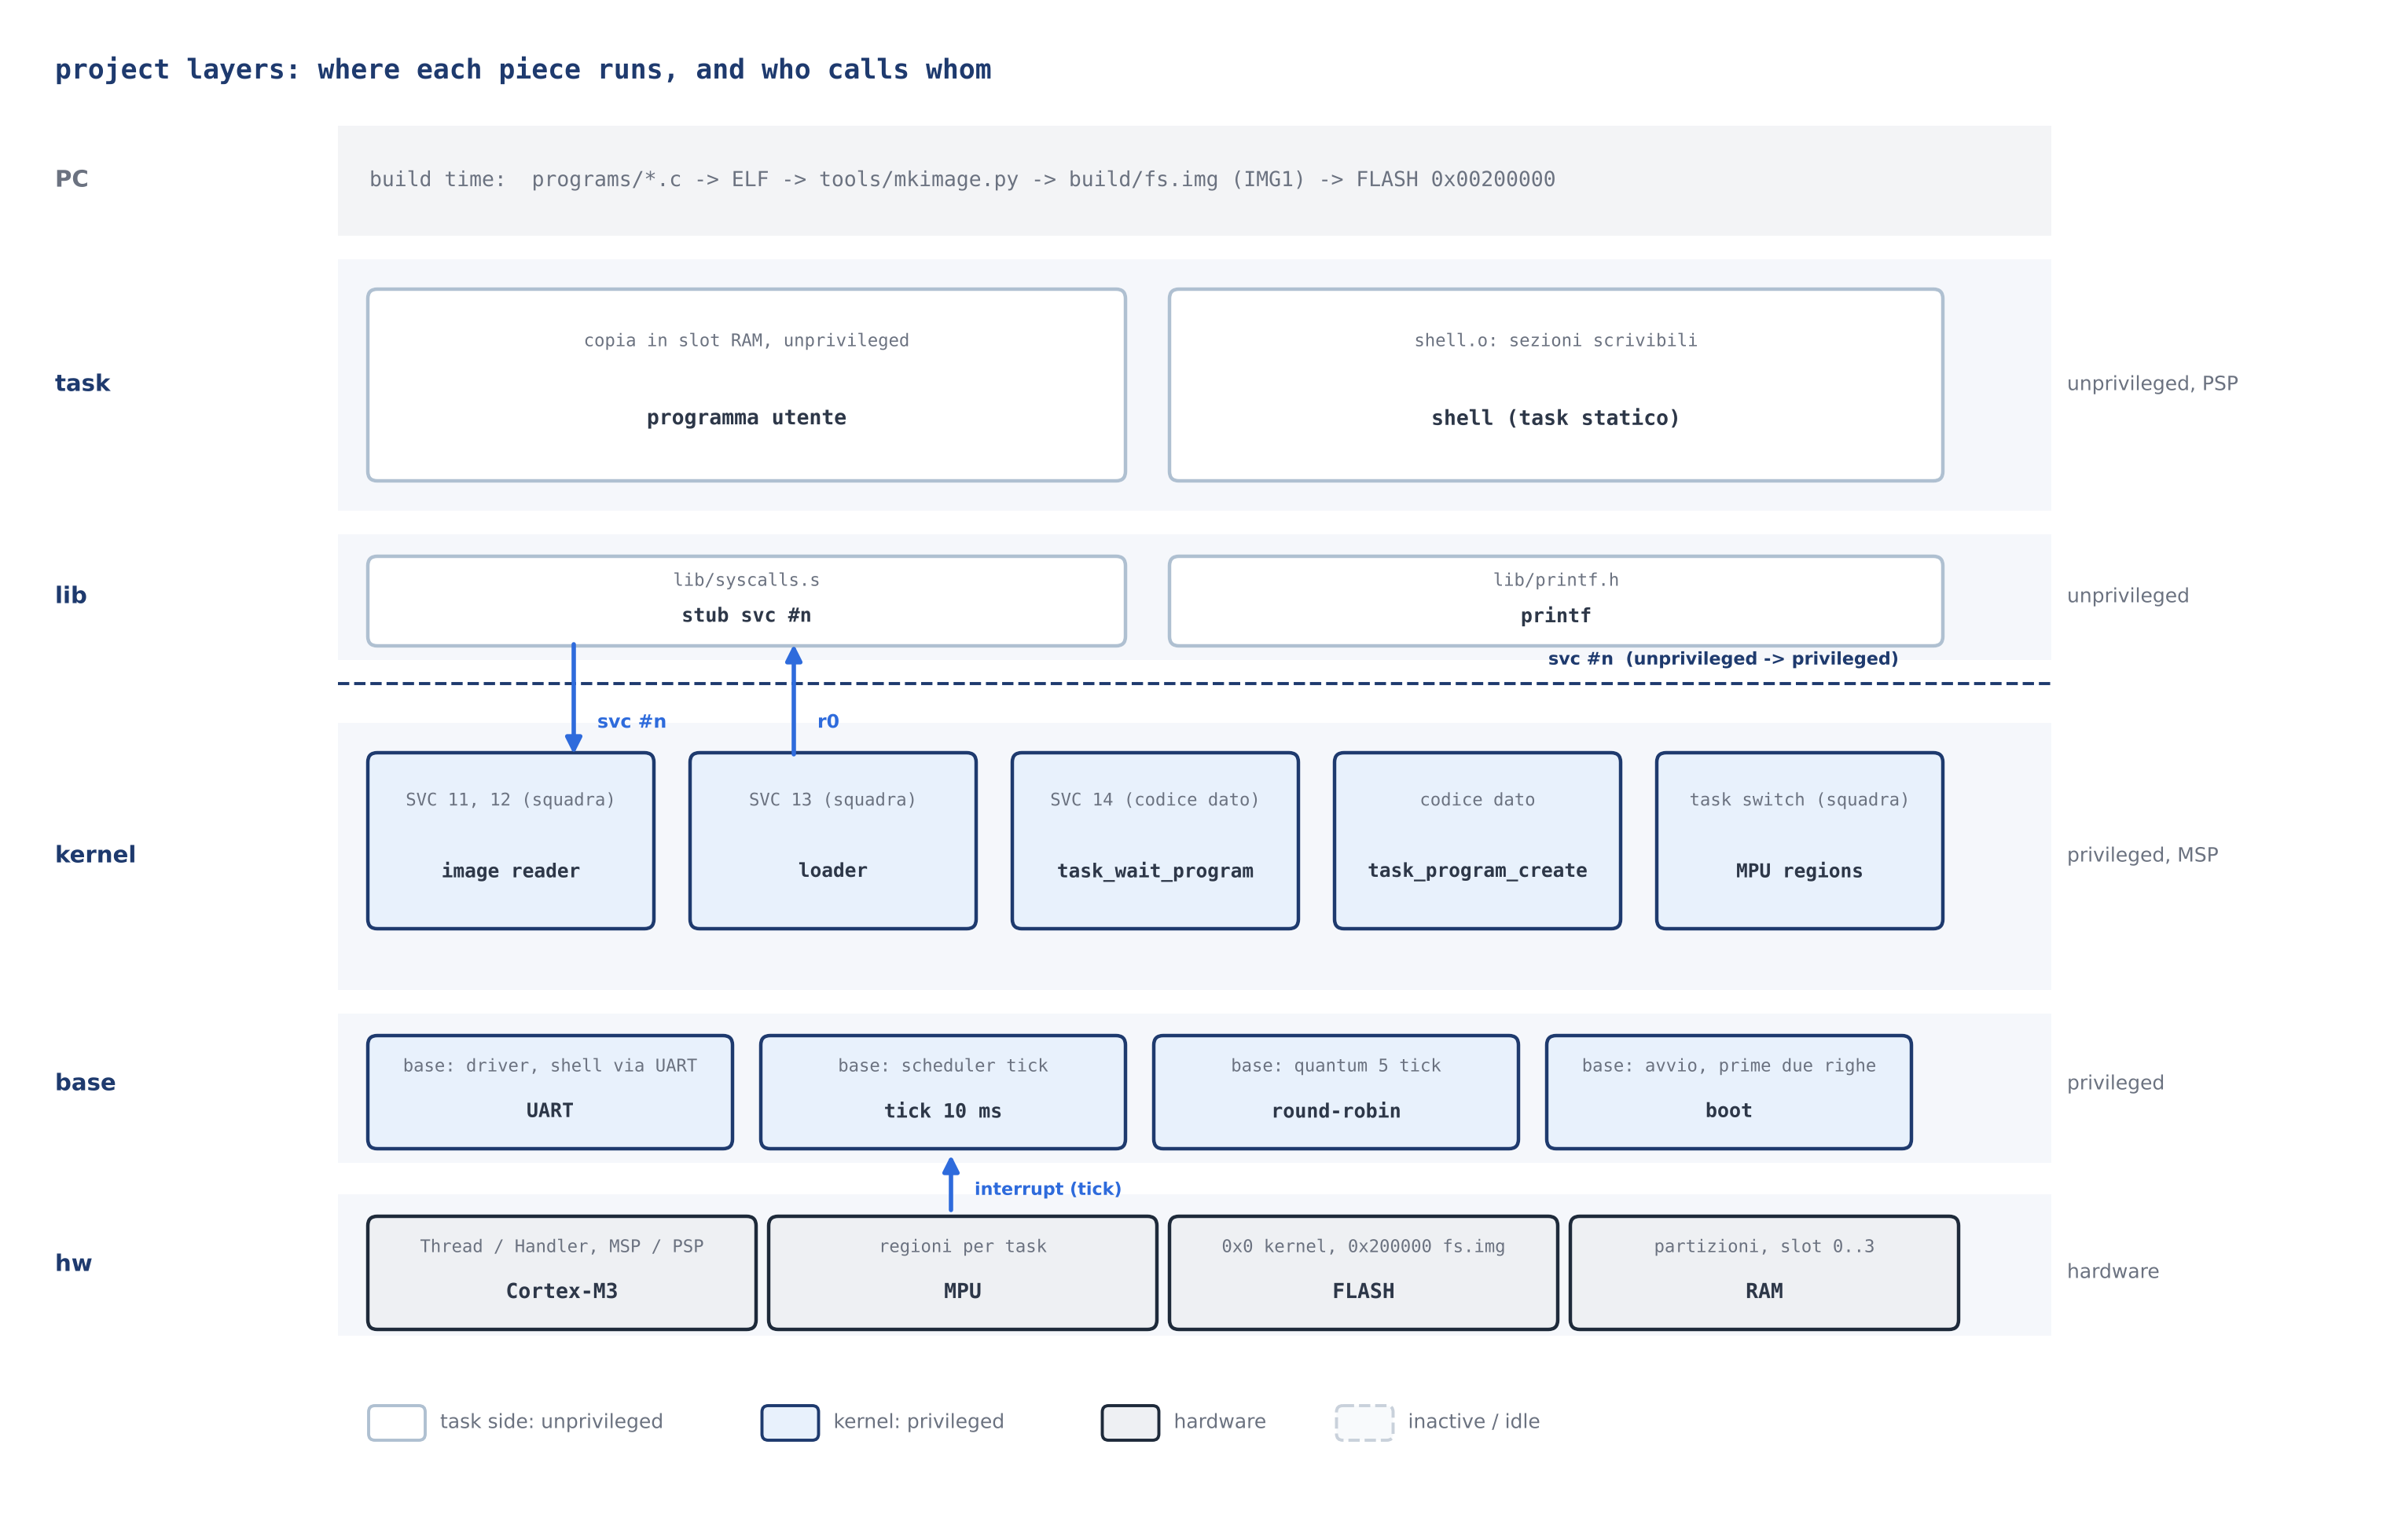
\includegraphics[width=1\textwidth]{contents/images/project/prj_layers.png}
    \caption{Stratificazione del sistema: i programmi utente girano unprivileged nel proprio slot di RAM, la shell è un task statico e il kernel privilegiato contiene loader, SVC 11--14 e MPU. Le frecce \texttt{svc} portano il controllo verso il kernel, il ritorno verso i programmi, e il tick arriva dall'hardware.}
    
\end{figure}

\subsection{Il sistema in due tempi}

Il lavoro si divide tra il PC (build time) e la board emulata da QEMU (run time):
\begin{enumerate}
\item sul PC, ogni \texttt{programs/*.c} passa dal compilatore e dal linker dei programmi e diventa un file programma;
\item sempre sul PC, l'host tool (\texttt{mkimage.py}) impacchetta tutti i file programma in \texttt{fs.img}, in formato IMG1;
\item in QEMU, la FLASH da \texttt{0x00000000} contiene kernel e shell, mentre la FLASH da \texttt{0x00200000} contiene \texttt{fs.img}, in sola lettura;
\item a run time la catena è: UART $\rightarrow$ shell $\rightarrow$ SVC $\rightarrow$ ricerca del programma $\rightarrow$ slot di RAM libero $\rightarrow$ copia, BSS a zero, relocation $\rightarrow$ MPU e creazione del task;
\item il programma gira unprivileged; quando finisce (return, exit o fault) lo slot si libera e la shell si risveglia.
\end{enumerate}

\begin{figure}[H]
    \centering
    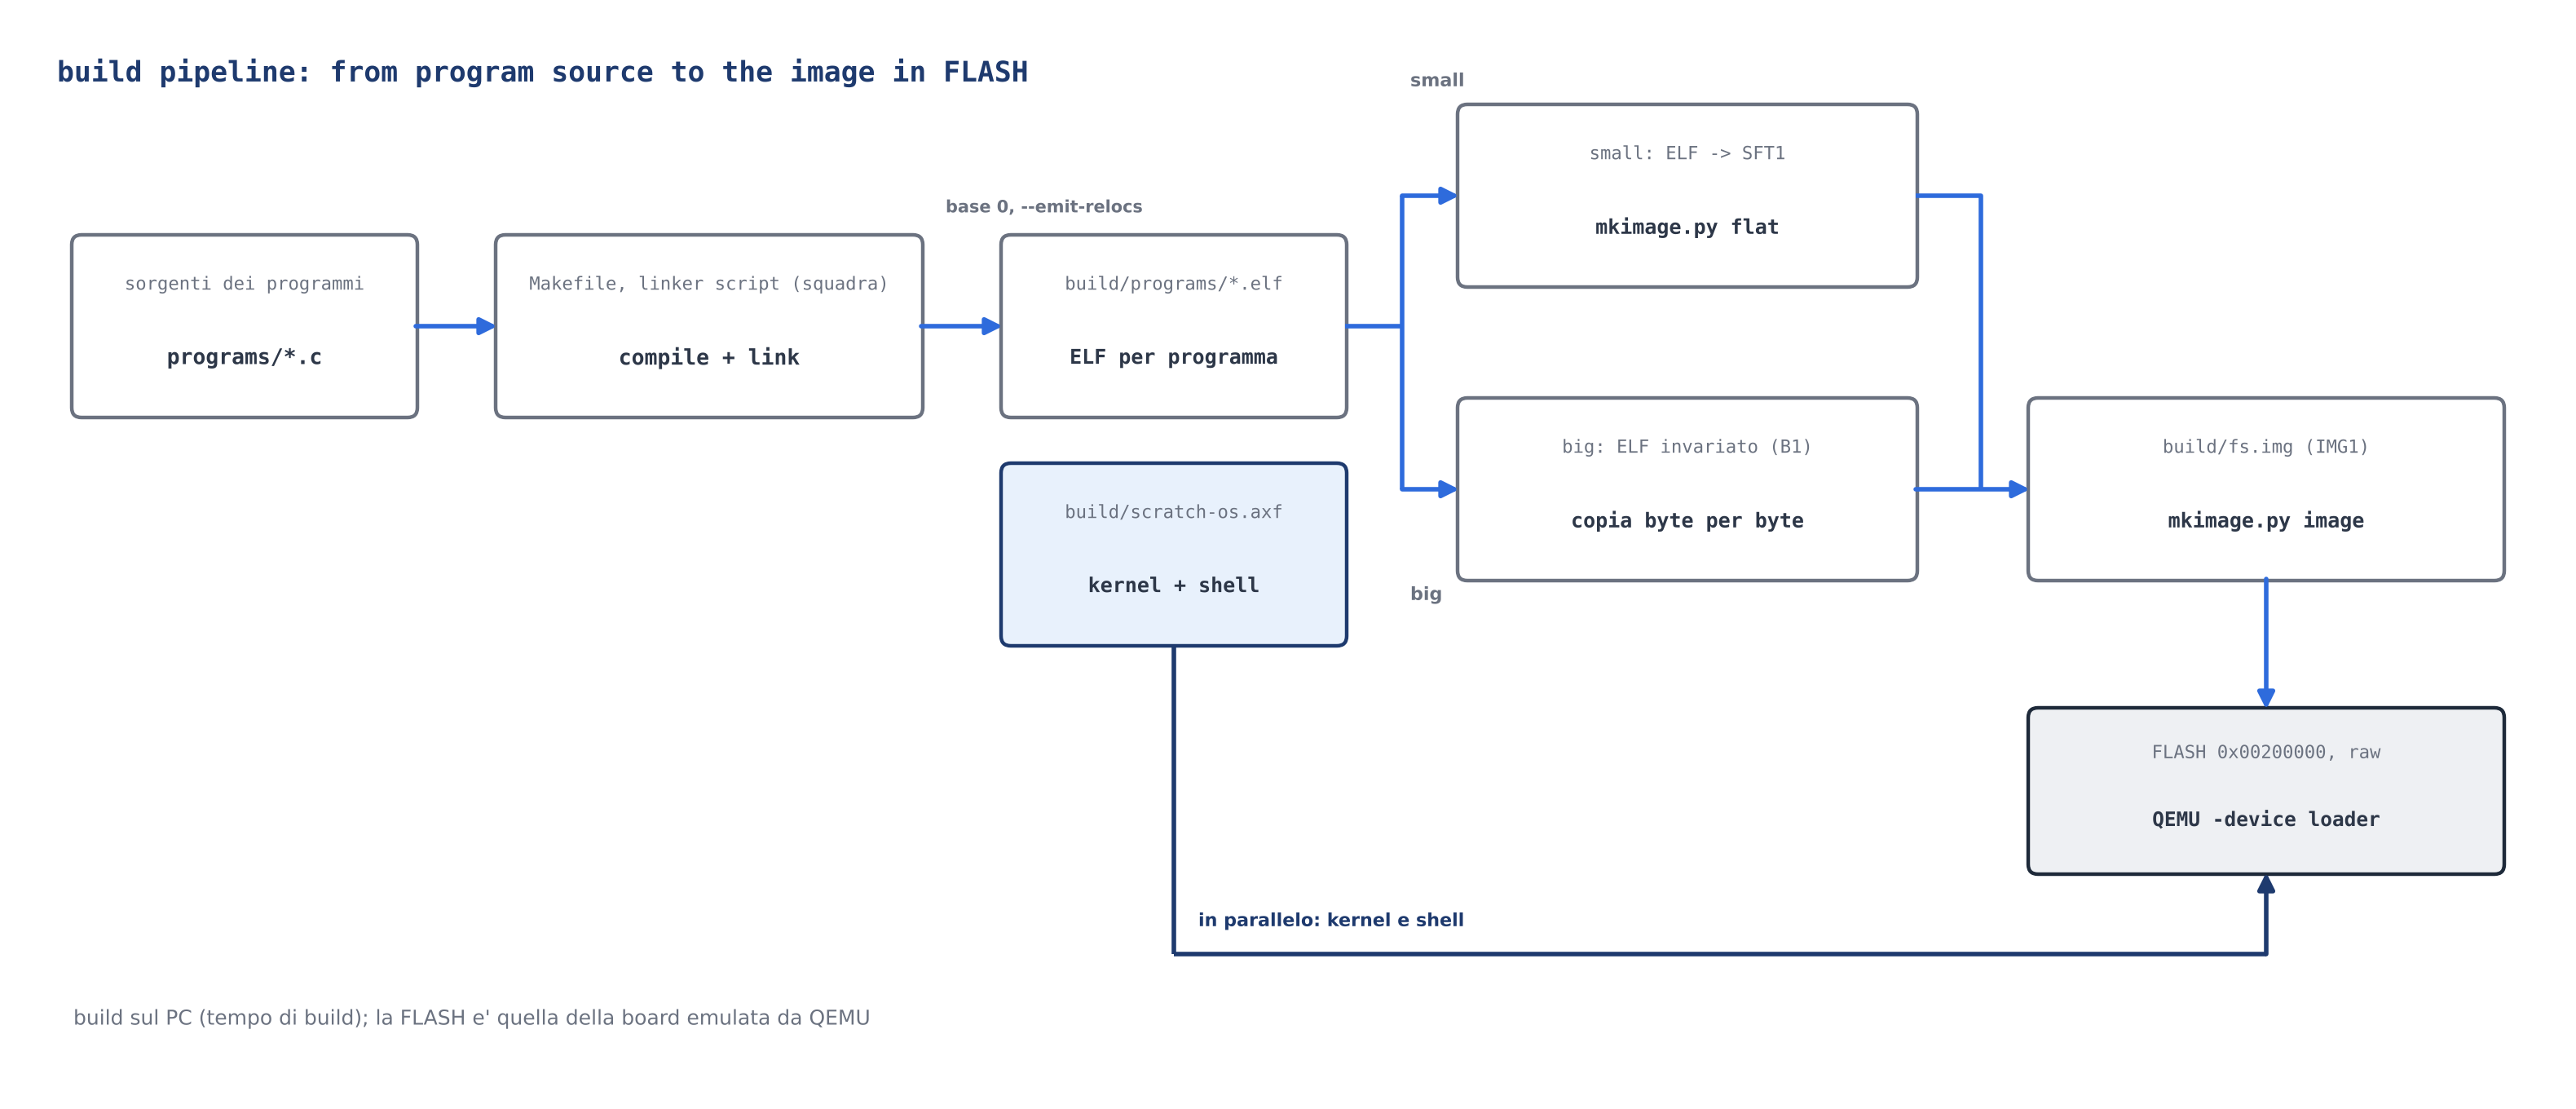
\includegraphics[width=1\textwidth]{contents/images/project/prj_build_pipeline.png}
    \caption{Dal sorgente all'immagine in FLASH: ogni programma è compilato e linkato a indirizzo 0 con \texttt{--emit-relocs}, e l'host tool crea \texttt{build/fs.img} in formato IMG1. Nella small i programmi entrano come SFT1, nella big come ELF invariati.}
    
\end{figure}

\subsection{Che cosa è dato e che cosa scrive la squadra}

Il codice dato, da usare e non da riscrivere, comprende:
\begin{itemize}
    \item i task record per quattro programmi caricati e i task id;
    \item l'attesa della fine di un programma e il report di come è finito;
    \item la gestione dell'exit e dei fault dei programmi;
    \item la system call 14.
\end{itemize}

La sua interfaccia è descritta in . La squadra scrive invece:
\begin{itemize}
    \item la shell e le system call da 11 a 13;
    \item la lettura dell'immagine e il controllo dei file programma;
    \item la copia e la relocation dei programmi;
    \item le impostazioni MPU di uno slot;
    \item startup texttt, linker script e regole di build dei programmi;
    \item l'host tool \texttt{tools/mkimage.py}.
\end{itemize}

\section{Le idee che servono}

\subsection{Perché un programma caricato va corretto}

Quando il linker costruisce un programma, fissa l'indirizzo di ogni funzione e di ogni variabile globale. Per un programma caricato a run time questo indirizzo non si conosce in anticipo: dipende da quale area di RAM è libera in quel momento. Per questo il programma si linka come se partisse dall'indirizzo \texttt{0}, e il loader lo copia dall'immagine in uno slot di RAM prima di eseguirlo.

La maggior parte delle istruzioni non dipende dall'indirizzo: un salto del tipo ``avanti di 40 byte'' funziona ovunque. Alcuni valori però contengono un indirizzo completo, per esempio un puntatore a una variabile globale o una tabella di puntatori a funzione. Questi valori sono giusti solo per l'indirizzo \texttt{0}: se il loader copia il programma a \texttt{0x20003000}, deve sommare \texttt{0x20003000} a ciascuno di essi.

Questa correzione si chiama \textbf{relocation} e l'elenco dei punti da correggere è la \textbf{relocation list}. Il linker produce questo elenco quando si linka con l'opzione \texttt{--emit-relocs}. Il Cortex-M3 non ha MMU (niente memoria virtuale), quindi non c'è un modo automatico per far girare un programma a un altro indirizzo: bisogna correggerlo.

\begin{figure}[H]
    \centering
    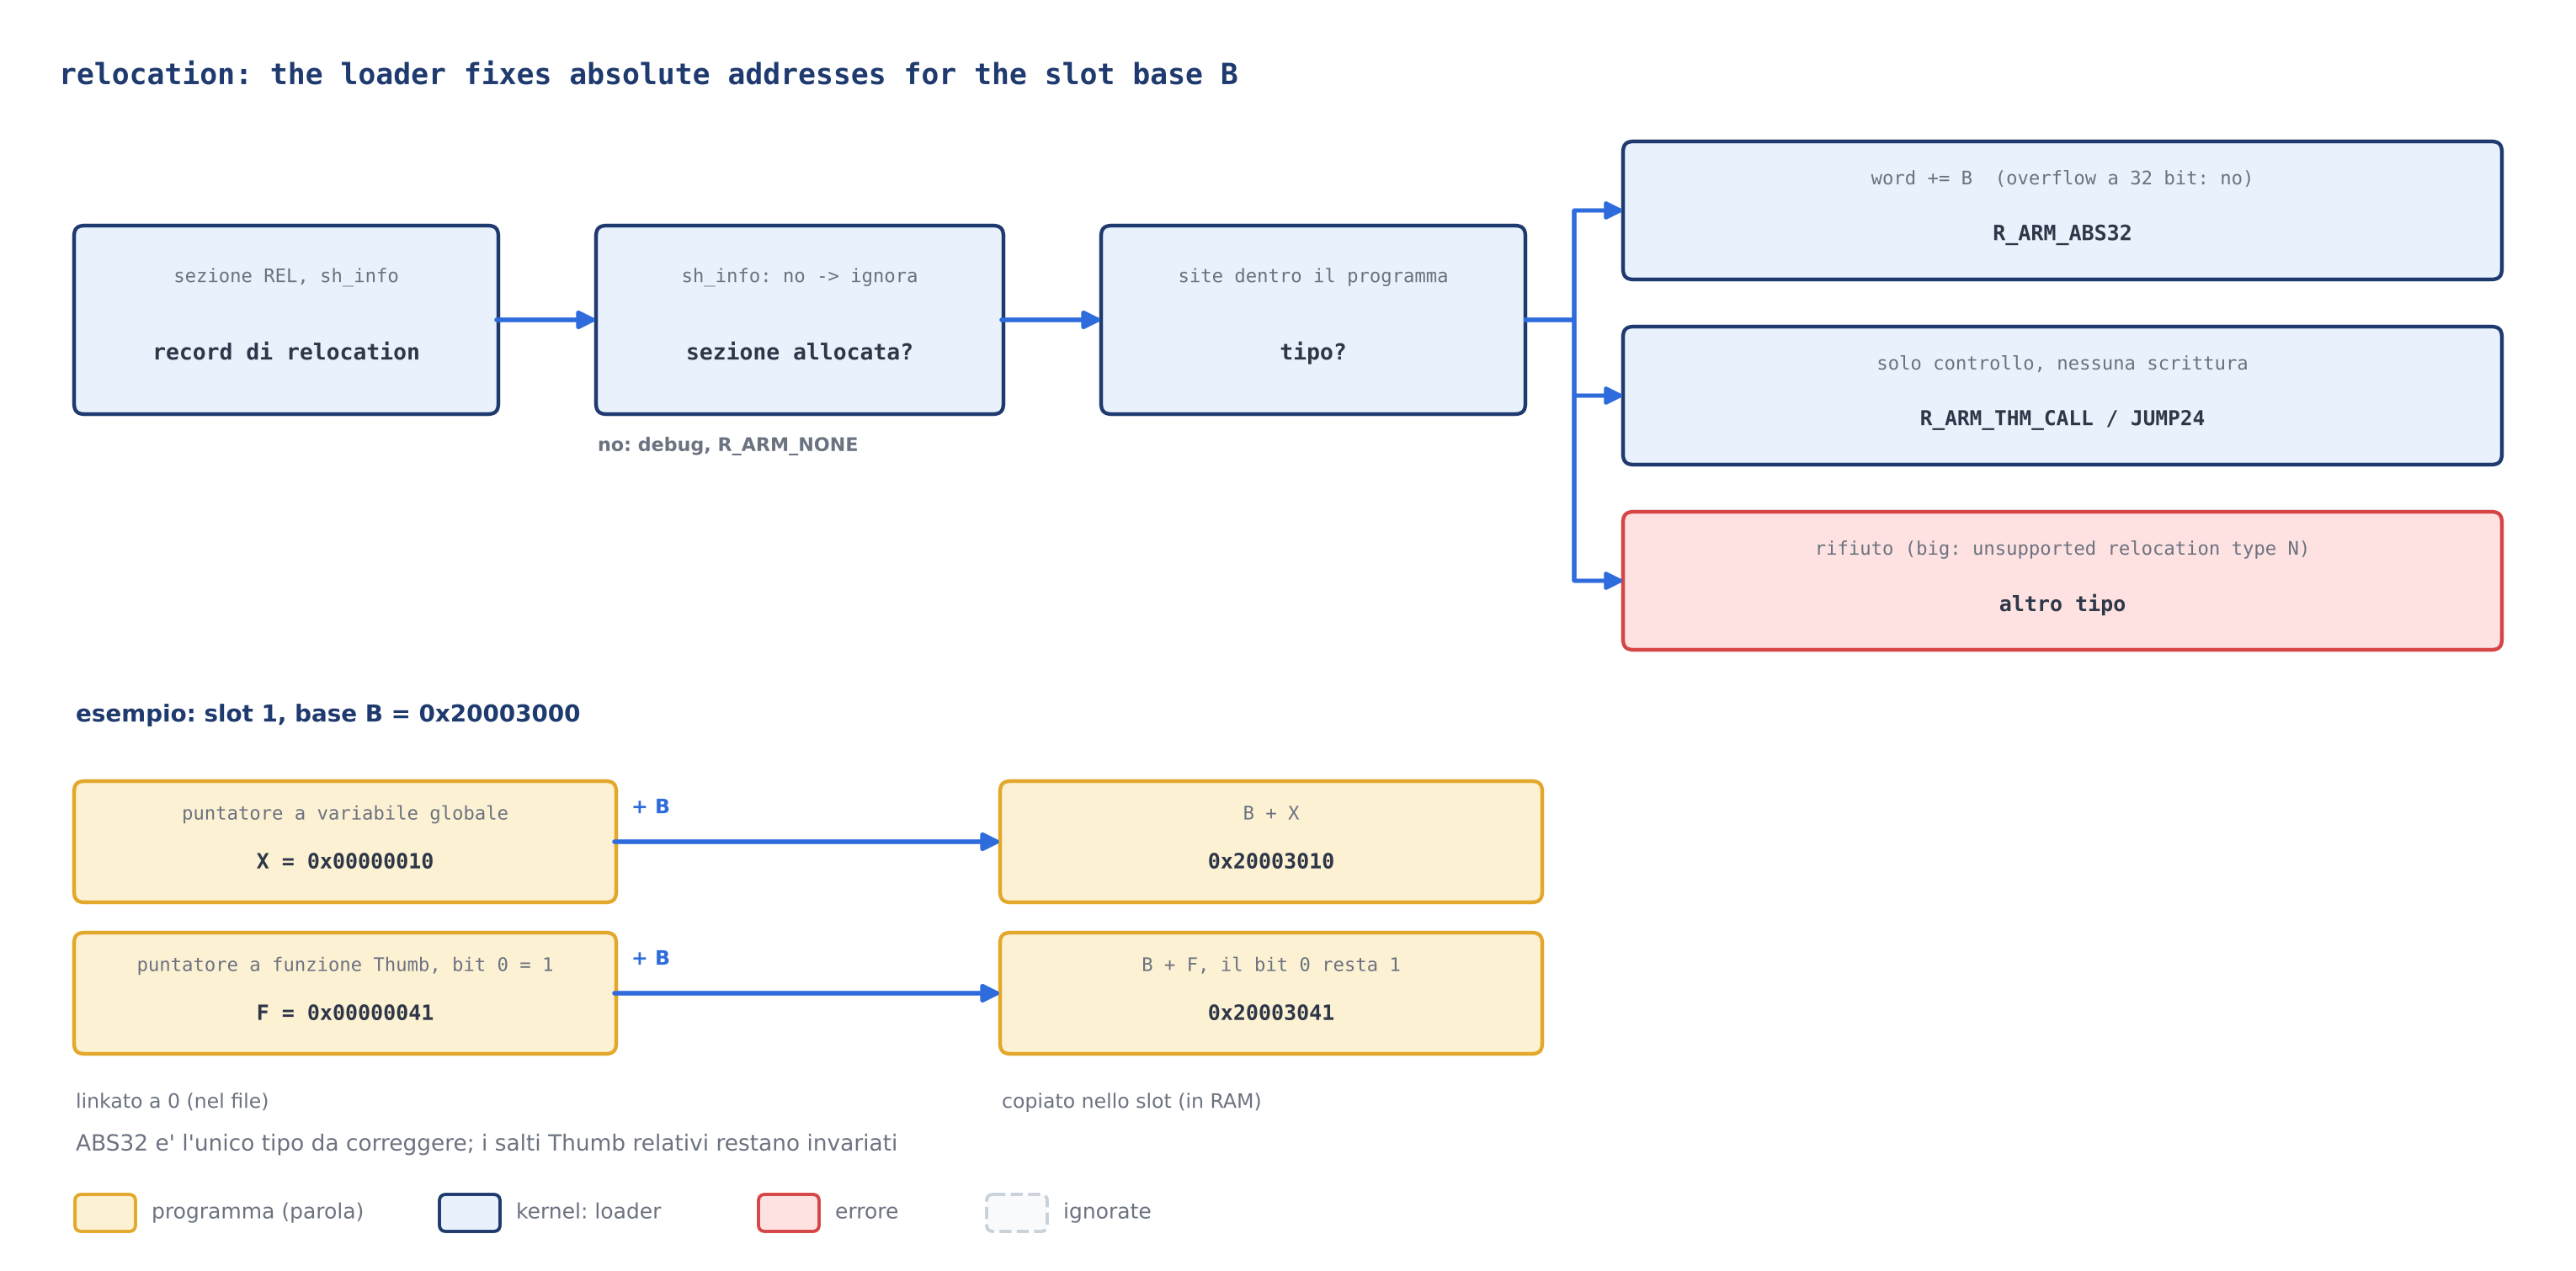
\includegraphics[width=1\textwidth]{contents/images/project/prj_relocation.png}
    \caption{Correzione degli indirizzi: ogni record di una sezione allocata viene applicato secondo il suo tipo. Nell'esempio il loader sposta i puntatori di un programma nello slot 1, sommando la base \texttt{0x20003000}.}
    
\end{figure}

\subsection{Le parti di un programma}

Un programma in memoria ha quattro parti:
\begin{itemize}
\item \textbf{texttt}: istruzioni e costanti read-only, per esempio le stringhe;
\item \textbf{data}: variabili globali con un valore iniziale, come \texttt{int x = 5;};
\item \textbf{BSS}: variabili globali che partono da zero, come \texttt{int y;}. Il file non contiene questi byte ma solo la loro dimensione, e il loader riempie l'area di zeri;
\item \textbf{stack}: usato mentre il programma gira.
\end{itemize}

\subsection{Magic number e versione}
Un file è solo una sequenza di byte. Per riconoscerne il formato, quasi tutti i formati binari iniziano con pochi byte fissi, il \textbf{magic number} (o \emph{magic}). Chi legge il file confronta prima questi byte: se non coincidono con quelli attesi, il file non è in quel formato (o è danneggiato) e viene rifiutato subito.

Ogni file ELF, per esempio, inizia con i quattro byte \texttt{7f 45 4c 46} (\texttt{0x7f} seguito dalle lettere \texttt{ELF}). Il progetto usa due formati propri: un'immagine inizia con le quattro lettere ASCII \texttt{IMG1}, un file programma \texttt{SFT1} con le lettere \texttt{SFT1}. Subito dopo la magic, entrambi i formati contengono un numero di \textbf{versione}, così il formato può cambiare in futuro senza essere confuso con il vecchio. Nel progetto la versione vale sempre \texttt{1}.

\subsection{Le parti di un file ELF che servono}

Il linker di GCC produce file ELF. Non serve conoscere tutto lo standard, solo queste parti:
\begin{itemize}
\item l'\textbf{ELF header}, all'inizio del file: contiene la magic, il tipo di file, l'entry point e la posizione delle due tabelle seguenti;
\item la \textbf{program header table}, che descrive i \textbf{segmenti}, cioè i pezzi del file da mettere in memoria per eseguire il programma. Un segmento di tipo \texttt{PT\_LOAD} va caricato;
\item la \textbf{section header table}, che descrive le \textbf{sezioni}, i pezzi più fini su cui lavora il linker: \texttt{.text} (codice), \texttt{.rodata} (costanti), \texttt{.data} e \texttt{.bss}. Una sezione è \textbf{allocated} quando occupa memoria mentre il programma gira (le informazioni di debug, per esempio, non lo sono). Una sezione di tipo \texttt{SHT\_NOBITS} occupa memoria ma nessun byte nel file: è così che è memorizzato il BSS;
\item le sezioni di relocation di tipo \texttt{REL}: ognuna contiene i record di relocation di un'altra sezione, indicata dal suo campo \texttt{sh\_info}. Ogni record dà una posizione (il \emph{site}), un simbolo e un \textbf{tipo di relocation}, che dice come calcolare l'indirizzo.
\end{itemize}

Il progetto usa solo tre tipi di relocation: \texttt{R\_ARM\_ABS32}, un indirizzo completo a 32 bit, e \texttt{R\_ARM\_THM\_CALL} e \texttt{R\_ARM\_THM\_JUMP24}, salti Thumb relativi alla posizione corrente. Di solito il linker toglie questi record dal file finale; \texttt{--emit-relocs} gli chiede di tenerli, così il loader li può usare. Tutte queste parti si vedono con \texttt{arm-none-eabi-readelf} ().

\subsection{Indirizzi Thumb}
Il Cortex-M3 esegue solo istruzioni Thumb. In ARM l'indirizzo di una funzione Thumb ha il bit più basso (bit 0) a 1. Quando il loader corregge un puntatore a funzione sommando l'indirizzo base, il bit 0 deve restare com'è.

\subsection{Protezione della memoria e W\textasciicircum{}X}
I programmi caricati girano unprivileged. La MPU deve impedire a un programma di toccare il kernel o la memoria di un altro programma. La versione big chiede anche la regola \textbf{W\textasciicircum{}X} (``write xor execute''): un'area di memoria può essere scrivibile o eseguibile, mai le due cose insieme. Con W\textasciicircum{}X un programma non può sovrascrivere il proprio codice né eseguire byte che stanno nei suoi dati o nello stack.

\subsection{Glossario}
\begin{center}
    \small
    \begin{tabular}{|p{0.22\linewidth}|p{0.66\linewidth}|}
        \hline
        \raggedright Termine & \raggedright Significato nel progetto \tabularnewline
        \hline\hline
        \raggedright Slot & \raggedright Area fissa di RAM da 4 KiB in cui vive un programma caricato. Gli slot sono quattro. \tabularnewline
        \hline
        \raggedright Magic number & \raggedright Byte fissi all'inizio di un file che ne identificano il formato. \tabularnewline
        \hline
        \raggedright Segmento, sezione & \raggedright Pezzi di un file ELF: i segmenti dicono che cosa caricare, le sezioni sono i pezzi più fini del linker (codice, costanti, dati, BSS, debug). \tabularnewline
        \hline
        \raggedright Sezione allocated & \raggedright Sezione che occupa memoria mentre il programma gira. \tabularnewline
        \hline
        \raggedright Immagine, IMG1 & \raggedright File read-only in FLASH che contiene tutti i file programma e una directory con i loro nomi. \tabularnewline
        \hline
        \raggedright SFT1 & \raggedright Formato semplice dei file programma della versione small, prodotto dall'host tool della squadra. \tabularnewline
        \hline
        \raggedright ELF & \raggedright Formato standard dei file prodotti dal linker di GCC. \tabularnewline
        \hline
        \raggedright Relocation & \raggedright Parola del programma che contiene un indirizzo e che il loader deve correggere. \tabularnewline
        \hline
        \raggedright BSS & \raggedright Variabili globali che partono da zero e non sono memorizzate nel file. \tabularnewline
        \hline
        \raggedright W\textasciicircum{}X & \raggedright Un'area di memoria è scrivibile oppure eseguibile, non entrambe le cose. \tabularnewline
        \hline
        \raggedright Task id & \raggedright Numero che identifica un programma caricato in esecuzione. Combina il numero dello slot con un contatore, la \textbf{generation}, che cresce a ogni riuso dello slot: così un id vecchio non coincide mai con un nuovo programma nello stesso slot. \tabularnewline
        \hline
    \end{tabular}
\end{center}

\section{Che cosa bisogna fare: i requisiti}
I requisiti dicono \emph{che cosa} deve fare il sistema, non in che ordine lavorare: il .md precisa che non sono un piano di lavoro e che ordine e divisione dei compiti li decide la squadra (una proposta di ordine è in ). R1--R9 valgono per entrambe le versioni, B1 e B2 solo per la big. Per la propria versione sono tutti obbligatori; opzionali sono solo il progetto stesso e gli extra in fondo alla tabella riassuntiva ().

\subsection{R1: programmi compilati separatamente dal kernel}
\begin{description}\sloppy
    \item[Che cosa chiede] Startup texttt, linker script e regole di build che compilano ogni programma di \texttt{programs/} in un proprio file ELF, linkato all'indirizzo \texttt{0} con \texttt{--emit-relocs}. Un programma non condivide codice con il kernel: ognuno include il proprio startup texttt, i propri stub delle system call, \texttt{printf} e ogni helper del compilatore che gli serve. \texttt{\_start} chiama \texttt{main}, e tornare da \texttt{main} chiude il programma come se avesse chiamato \texttt{sys\_exit()}. La build crea i programmi e \texttt{build/fs.img} dai sorgenti, con GCC ARM bare-metal, ogni volta nello stesso modo.
    \item[Perché serve] Un programma caricato a run time non conosce il proprio indirizzo: linkato a \texttt{0} e con le relocation conservate, può essere spostato in qualunque slot. Non condividendo codice con il kernel, è un file davvero autonomo.
    \item[Dove si interviene] I sorgenti in \texttt{programs/}; startup texttt e linker script dei programmi (nomi scelti dalla squadra); il Makefile (dettagli scelti dalla squadra); gli stub di \texttt{lib/syscalls.s} e \texttt{lib/printf.h}. Nell'esempio di debug del .md un programma compilato si trova in \texttt{build/programs/thumb\_ptr.elf}. Dettagli in  e .
    \item[Come si verifica] Con \texttt{arm-none-eabi-readelf} si controlla che ogni ELF sia di tipo \texttt{ET\_EXEC}, con entry point Thumb, almeno un segmento \texttt{PT\_LOAD} e le sezioni \texttt{REL}. I test \texttt{normal\_return} ed \texttt{explicit\_exit} controllano il ritorno da \texttt{main} e la chiamata a \texttt{sys\_exit}. Una build da zero deve ricreare programmi e immagine.
\end{description}

\subsection{R2: un host tool impacchetta i programmi}
\begin{description}\sloppy
    \item[Che cosa chiede] Scrivere \texttt{tools/mkimage.py}. Lo strumento costruisce \texttt{build/fs.img}, in formato IMG1, da una lista di programmi, e rifiuta l'input sbagliato con un messaggio d'errore chiaro. Le squadre small implementano anche la conversione da ELF a SFT1.
    \item[Perché serve] Il kernel deve trovare tutti i programmi in un solo file in FLASH, in un formato fisso che conosce anche il test kit.
    \item[Dove si interviene] \texttt{tools/mkimage.py}; la ricetta \texttt{make image} della base, da adattare (); il risultato \texttt{build/fs.img}. Dettagli in ,  e .
    \item[Come si verifica] In caso di successo lo strumento stampa esattamente i messaggi previsti (); con un input sbagliato scrive \texttt{mkimage.py:\ error:\ <reason>} su standard error ed esce con stato 2, senza scrivere output. In QEMU, \texttt{ls} elenca i programmi impacchettati.
\end{description}

\subsection{R3: il kernel legge l'immagine sul posto}
\begin{description}\sloppy
    \item[Che cosa chiede] Il kernel trova l'immagine all'indirizzo FLASH \texttt{0x00200000}, la controlla e cerca i programmi per nome. La legge dov'è: non ci scrive mai e non la copia mai intera in RAM.
    \item[Perché serve] L'immagine emula un disco esterno in sola lettura; copiarla sprecherebbe RAM, e l'efficienza è valutata (niente copie inutili dell'immagine).
    \item[Dove si interviene] Il codice del kernel che legge e controlla l'immagine (modulo e nomi scelti dalla squadra), che la trova tramite il simbolo del linker \texttt{\_\_fs\_image\_start}. Dettagli in .
    \item[Come si verifica] \texttt{ls} elenca i nomi nell'ordine della directory. Con un'immagine non valida, come il segnaposto della base, \texttt{ls} stampa \texttt{error:\ no valid image}, \texttt{run} stampa \texttt{error:\ program cannot be loaded} e la shell continua a funzionare.
\end{description}

\subsection{R4: una shell per elencare e avviare i programmi}
\begin{description}\sloppy
    \item[Che cosa chiede] La shell è un task statico che legge righe dalla UART e accetta i comandi \texttt{help}, \texttt{ls} e \texttt{run <name>}. Stampa esattamente il prompt e i messaggi di . Mentre un programma gira, aspetta senza stampare il prompt.
    \item[Perché serve] È l'interfaccia verso l'utente e verso il test kit, che confronta ogni carattere stampato.
    \item[Dove si interviene] Il sorgente della shell (le sue sezioni scrivibili vengono da \texttt{shell.o}); la configurazione del task con \texttt{task\_project\_configure()} e \texttt{task\_configure\_shell()}; i simboli del linker della shell ().
    \item[Come si verifica] Le trascrizioni del test kit contengono prompt, eco e messaggi di ogni test. A mano: una riga vuota, \texttt{run} da solo o \texttt{help} seguito da altri caratteri devono stampare \texttt{error:\ unknown command}; una riga lunga si ferma a 31 caratteri.
\end{description}

\subsection{R5: i programmi si avviano con system call}
\begin{description}\sloppy
    \item[Che cosa chiede] La shell usa le system call da 11 a 14 per contare i programmi, leggerne i nomi, avviarne uno e aspettarne la fine. I risultati devono essere esattamente quelli di .
    \item[Perché serve] La shell non tocca direttamente immagine e task: passa dal kernel con una SVC. Le stesse chiamate le usa anche un programma caricato che avvia un altro programma (test \texttt{nonzero\_slot\_relocation}).
    \item[Dove si interviene] Le SVC 11, 12 e 13 nel kernel (la 14 è già data); gli stub lato utente, come quelli di \texttt{lib/syscalls.s}. \emph{Da chiarire con il professore:} il .md non dice se \texttt{lib/syscalls.s} contiene già gli stub delle SVC 11--14 o se vanno aggiunti.
    \item[Come si verifica] Ogni caso d'errore restituisce il codice giusto (\texttt{-1}, \texttt{-2}, \texttt{-3}, \texttt{-4}) e la shell stampa il messaggio corrispondente. Nel test \texttt{nonzero\_slot\_relocation} il programma padre riceve 0.
\end{description}

\subsection{R6: il loader mette il programma in uno slot libero e lo fa funzionare lì}
\begin{description}\sloppy
    \item[Che cosa chiede] Per \texttt{run <name>} il kernel sceglie il primo slot libero, copia codice e dati nello slot, riempie di zeri il BSS, somma l'indirizzo dello slot a ogni parola della relocation list, controlla entry point e stack, e solo allora crea il task.
    \item[Perché serve] È il cuore del progetto ed è il criterio che vale di più (2.50 punti).
    \item[Dove si interviene] Il loader nel kernel (scritto dalla squadra); le funzioni date \texttt{task\_program\_slot\_free(slot)} e \texttt{task\_program\_create(slot, name, entry, stack\_top, executable)}; i simboli del linker degli slot. Dettagli in  (small),  (big) e .
    \item[Come si verifica] La riga \texttt{loader:} riporta slot, base e id corretti. I test \texttt{global\_state} (globali, BSS e costanti), \texttt{thumb\_ptr} (puntatore a funzione Thumb), \texttt{nonzero\_slot\_relocation} (relocation nello slot 1) e \texttt{too\_large} (programma troppo grande) controllano i casi principali.
\end{description}
\emph{Da chiarire con il professore:} il .md non elenca uno per uno i controlli sullo stack. Da  si sa che il programma occupa al massimo i 3072 byte bassi dello slot, che lo stack occupa i 1024 byte alti, che lo stack pointer iniziale è la fine dello slot e che i frame iniziali usano i 64 byte in cima.

\subsection{R7: un programma può toccare solo il proprio slot}
\begin{description}\sloppy
    \item[Che cosa chiede] Un programma caricato esegue sempre dal proprio slot di RAM, dove il loader l'ha copiato: il file nell'immagine è solo la sorgente della copia. I programmi girano unprivileged e la MPU permette a un programma il proprio slot e nient'altro in RAM: né la RAM del kernel né altri slot. La FLASH resta leggibile ed eseguibile per tutti i task unprivileged, come nella base, perché la shell è un task statico con il codice in FLASH; la FLASH non si può scrivere, quindi la protezione non si indebolisce.
    \item[Perché serve] Un programma con un bug non deve poter corrompere il kernel o gli altri programmi: il suo errore diventa un fault recuperabile.
    \item[Dove si interviene] Le impostazioni MPU di uno slot; l'argomento \texttt{executable} di \texttt{task\_program\_create}; nella big anche il setup MPU fatto a ogni task switch. Dettagli in .
    \item[Come si verifica] Test \texttt{kernel\_store}: il programma scrive a \texttt{0x20000000} e il sistema stampa \texttt{MemManage in loaded program:\ CFSR=0x82 address=0x20000000}; poi \texttt{print\_plain} riusa lo slot 0 con id 8. Il professore consiglia anche di controllare i permessi risultanti dopo ogni task switch.
\end{description}

\subsection{R8: la fine di un programma libera il suo slot}
\begin{description}\sloppy
    \item[Che cosa chiede] Quando un programma torna da \texttt{main}, chiama \texttt{sys\_exit()} o provoca un fault recuperabile, il sistema stampa il messaggio corrispondente, libera subito lo slot e sveglia la shell, che mostra di nuovo il prompt. Questo comportamento si ottiene usando bene il codice dato (), non scrivendone una versione propria.
    \item[Perché serve] Gli slot sono solo quattro e devono tornare subito disponibili; il codice comune garantisce lo stesso comportamento in tutte le squadre.
    \item[Dove si interviene] Lato squadra: lo startup texttt (ritorno da \texttt{main}) e la shell, che chiama la SVC 14. Lato codice dato, da non toccare: \texttt{task\_wait\_program}, il codice della SVC 14, \texttt{task\_finish\_current}, \texttt{task\_fault\_current}, \texttt{task\_current\_is\_program}, l'entry dei fault e il dispatcher.
    \item[Come si verifica] Test \texttt{normal\_return}, \texttt{explicit\_exit} e \texttt{kernel\_store} (dopo il fault lo slot 0 viene riusato con id 8).
\end{description}

\subsection{R9: un input sbagliato non rompe mai il sistema}
\begin{description}\sloppy
\item[Che cosa chiede] Un'immagine danneggiata, un file programma danneggiato o un argomento sbagliato di una system call vengono rifiutati con l'errore giusto, prima che un solo byte del programma sia copiato o eseguito. Il kernel non va in crash, nessuno slot cambia e la shell continua a funzionare.
\item[Perché serve] Il kernel non può fidarsi di dati che vengono da fuori: l'immagine e gli argomenti passati da codice unprivileged.
\item[Dove si interviene] I controlli sull'immagine (), sui file SFT1 () o ELF () e sugli argomenti delle system call ().
\item[Come si verifica] Test \texttt{bad\_magic}, \texttt{bad\_header}, \texttt{too\_large} e \texttt{bad\_reloc}: dopo il rifiuto, \texttt{help} mostra che la shell funziona ancora. Nella big anche \texttt{unsupported\_reloc} e \texttt{truncated\_elf}.
\end{description}

\subsection{B1 (solo big): il kernel carica file ELF}
\begin{description}\sloppy
\item[Che cosa chiede] L'immagine contiene ogni file ELF esattamente come l'ha prodotto il linker, e l'host tool si limita a impacchettare. È il kernel a controllare l'ELF, a trovare le parti da caricare e le relocation, e ad applicarle.
\item[Perché serve] È il lavoro di un loader vero: niente formato intermedio preparato sul PC.
\item[Dove si interviene] Il lettore ELF nel kernel (struttura scelta dalla squadra) e il comando \texttt{image} di \texttt{tools/mkimage.py}, che copia gli ELF byte per byte. Dettagli in .
\item[Come si verifica] La suite big esegue i dieci test comuni con file ELF, più \texttt{unsupported\_reloc} (stampa \texttt{loader:\ unsupported relocation type 3}) e \texttt{truncated\_elf}. Se B1 manca o non funziona: penalità di $-2.00$ punti.
\end{description}

\subsection{B2 (solo big): codice e dati protetti separatamente}
\begin{description}\sloppy
\item[Che cosa chiede] La regola W\textasciicircum{}X: il codice si può leggere ed eseguire ma non scrivere; dati e stack si possono leggere e scrivere ma non eseguire. Un programma che scrive nel proprio codice o salta nei propri dati si ferma con un memory fault recuperabile, come in R8.
\item[Perché serve] Impedisce a un programma di modificare il proprio codice e di eseguire byte scritti nei dati o nello stack.
\item[Dove si interviene] Le regioni MPU (quali usare lo decide la squadra). Le squadre big possono aggiungere campi ai task record ed estendere il setup MPU fatto a ogni task switch. L'argomento \texttt{executable} da solo non basta per W\textasciicircum{}X.
\item[Come si verifica] Test \texttt{wx\_write\_texttt} (\texttt{MemManage in loaded program:\ CFSR=0x82 address=0x20002280}) e \texttt{wx\_exec\_data} (\texttt{MemManage in loaded program:\ CFSR=0x1}); in entrambi un programma corretto riusa poi lo slot 0 con id 8. Se B2 manca, anche in una sola direzione: penalità di $-1.00$ punti, contata una volta sola.
\end{description}

\subsection{Tabella riassuntiva}

\begin{center}
\small
\setlength{\tabcolsep}{4pt}
\begin{tabular}{|p{0.14\linewidth}|p{0.17\linewidth}|p{0.26\linewidth}|p{0.32\linewidth}|}
\hline
\raggedright Requisito & \raggedright Obbligatorio? & \raggedright File coinvolti & \raggedright Come si verifica \tabularnewline
\hline\hline
\raggedright R1 Build dei programmi & \raggedright Sì, small e big & \raggedright \texttt{programs/}, startup texttt, linker script, Makefile, \texttt{lib/syscalls.s} & \raggedright \texttt{arm-none-eabi-readelf}; \texttt{normal\_return}, \texttt{explicit\_exit} \tabularnewline
\hline
\raggedright R2 Host tool & \raggedright Sì; \texttt{flat} solo small & \raggedright \texttt{tools/mkimage.py}, \texttt{build/fs.img} & \raggedright Messaggi esatti; errori con stato 2 \tabularnewline
\hline
\raggedright R3 Immagine sul posto & \raggedright Sì & \raggedright Lettore dell'immagine nel kernel & \raggedright \texttt{ls}; \texttt{error:\ no valid image} \tabularnewline
\hline
\raggedright R4 Shell & \raggedright Sì & \raggedright Sorgente di \texttt{shell.o}, simboli del linker della shell & \raggedright Trascrizioni del test kit \tabularnewline
\hline
\raggedright R5 System call 11--14 & \raggedright Sì & \raggedright SVC 11--13 nel kernel, stub & \raggedright Codici di ritorno; \texttt{nonzero\_\allowbreak slot\_\allowbreak relocation} \tabularnewline
\hline
\raggedright R6 Loader & \raggedright Sì & \raggedright Loader, \texttt{task\_\allowbreak program\_\allowbreak create} & \raggedright \texttt{global\_state}, \texttt{thumb\_ptr}, \texttt{too\_large} \tabularnewline
\hline
\raggedright R7 Isolamento MPU & \raggedright Sì & \raggedright Codice MPU & \raggedright \texttt{kernel\_store} \tabularnewline
\hline
\raggedright R8 Fine e riuso dello slot & \raggedright Sì, con il codice dato & \raggedright Startup texttt, shell; codice dato di \texttt{kernel/task.h} & \raggedright \texttt{normal\_return}, \texttt{explicit\_exit}, \texttt{kernel\_store} \tabularnewline
\hline
\raggedright R9 Rifiuto dell'input sbagliato & \raggedright Sì & \raggedright Tutti i controlli del kernel & \raggedright \texttt{bad\_magic}, \texttt{bad\_header}, \texttt{too\_large}, \texttt{bad\_reloc} \tabularnewline
\hline
\raggedright B1 ELF nel kernel & \raggedright Solo big (altrimenti $-2.00$) & \raggedright Lettore ELF, comando \texttt{image} & \raggedright \texttt{unsupported\_reloc}, \texttt{truncated\_elf} \tabularnewline
\hline
\raggedright B2 W\textasciicircum{}X & \raggedright Solo big (altrimenti $-1.00$) & \raggedright Codice MPU, task record & \raggedright \texttt{wx\_write\_texttt}, \texttt{wx\_exec\_data} \tabularnewline
\hline
\raggedright Extra & \raggedright Opzionali & \raggedright Programmi e test privati, test lato host, funzioni in più & \raggedright Non devono cambiare comandi, output, formati e test \tabularnewline
\hline
\end{tabular}
\end{center}

\section{Formati e messaggi esatti}

Questa sezione raccoglie i dettagli che devono essere identici in tutte le squadre, perché il test kit comune li controlla byte per byte.

Salvo indicazione diversa valgono tre convenzioni: ogni numero di più di un byte in IMG1 e SFT1 è un intero senza segno a 32 bit little-endian; gli offset si contano dal primo byte dell'immagine o del file; un intervallo scritto \texttt{[start, end)} contiene \texttt{start} ma non \texttt{end}.

\subsection{L'immagine IMG1}

\begin{sloppypar}
\paragraph{Dove si trova.} QEMU carica il file \texttt{build/fs.img} senza modificarlo, a partire dall'indirizzo FLASH \texttt{0x00200000} (l'opzione esatta è in ). L'immagine può occupare al massimo 2 MiB, cioè \texttt{0x00200000..0x003fffff}. Il kernel la legge lì, senza scriverla e senza copiarla.
\end{sloppypar}

\paragraph{Header.} L'immagine inizia con un header di esattamente 20 byte:

\begin{center}
\small
\begin{tabular}{|r|r|l|p{0.45\linewidth}|}
\hline
Byte & Dim. & Campo & \raggedright Valore \tabularnewline
\hline\hline
\texttt{0..3} & 4 & \texttt{magic} & \raggedright magic number dell'immagine: byte \texttt{49 4d 47 31} (\texttt{IMG1}), valore numerico \texttt{0x31474d49} \tabularnewline
\hline
\texttt{4..7} & 4 & \texttt{version} & \raggedright esattamente \texttt{1} \tabularnewline
\hline
\texttt{8..11} & 4 & \texttt{image\_size} & \raggedright dimensione totale dell'immagine, da 20 a \texttt{0x00200000} byte \tabularnewline
\hline
\texttt{12..15} & 4 & \texttt{count} & \raggedright numero di voci della directory, da 1 a 32 \tabularnewline
\hline
\texttt{16..19} & 4 & \texttt{directory\_offset} & \raggedright dove inizia la directory; multiplo di 4, almeno 20 \tabularnewline
\hline
\end{tabular}
\end{center}

Il valore \texttt{directory\_offset + count * 24} non deve andare in overflow e non deve superare \texttt{image\_size}. Il packer della squadra mette sempre la directory al byte 20.

\paragraph{Directory.} La directory ha esattamente \texttt{count} voci da 24 byte:

\begin{center}
\small
\begin{tabular}{|r|r|l|p{0.45\linewidth}|}
\hline
Byte & Dim. & Campo & \raggedright Valore \tabularnewline
\hline\hline
\texttt{0..15} & 16 & \texttt{name} & \raggedright nome del programma, seguito da un byte NUL \tabularnewline
\hline
\texttt{16..19} & 4 & \texttt{offset} & \raggedright dove inizia il file programma; multiplo di 4 \tabularnewline
\hline
\texttt{20..23} & 4 & \texttt{size} & \raggedright dimensione esatta del file programma, almeno 40 byte \tabularnewline
\hline
\end{tabular}
\end{center}

Un nome ha da 1 a 15 caratteri, scelti tra \texttt{A}--\texttt{Z}, \texttt{a}--\texttt{z}, \texttt{0}--\texttt{9}, \texttt{\_} e \texttt{-}. Due voci non possono avere lo stesso nome. Il kernel ignora i byte dopo il primo NUL; il packer li mette a zero e rifiuta i nomi duplicati.

\paragraph{File programma.} \texttt{contents\_start} è la fine della directory, arrotondata a un multiplo di 4. Ogni file inizia a \texttt{contents\_start} o dopo, ogni intervallo \texttt{[offset, offset + size)} sta dentro \texttt{image\_size} e due file non si sovrappongono mai. Le voci possono essere in qualunque ordine, tra un file e l'altro ci possono essere buchi e le dimensioni dei file non devono per forza essere multipli di 4.

\paragraph{Che cosa fa il packer.} Mantiene i file nell'ordine della riga di comando, allinea l'inizio di ciascuno con padding di zeri e pone \texttt{image\_size} uguale alla fine dell'ultimo file. Rifiuta zero file, più di 32 file e immagini più grandi di 2 MiB.

\paragraph{Che cosa fa il kernel con un'immagine sbagliata.} Se anche una sola di queste regole è violata, l'intera immagine non è valida, e allora:
\begin{itemize}\sloppy
\item \texttt{ls} stampa \texttt{error:\ no valid image};
\item \texttt{run <name>} stampa \texttt{error:\ program cannot be loaded};
\item la shell continua a funzionare.
\end{itemize}
Un'immagine valida può comunque contenere un file programma rotto: \texttt{ls} lo elenca, e \texttt{run} trova il problema quando controlla il file.

\begin{figure}[H]
    \centering
    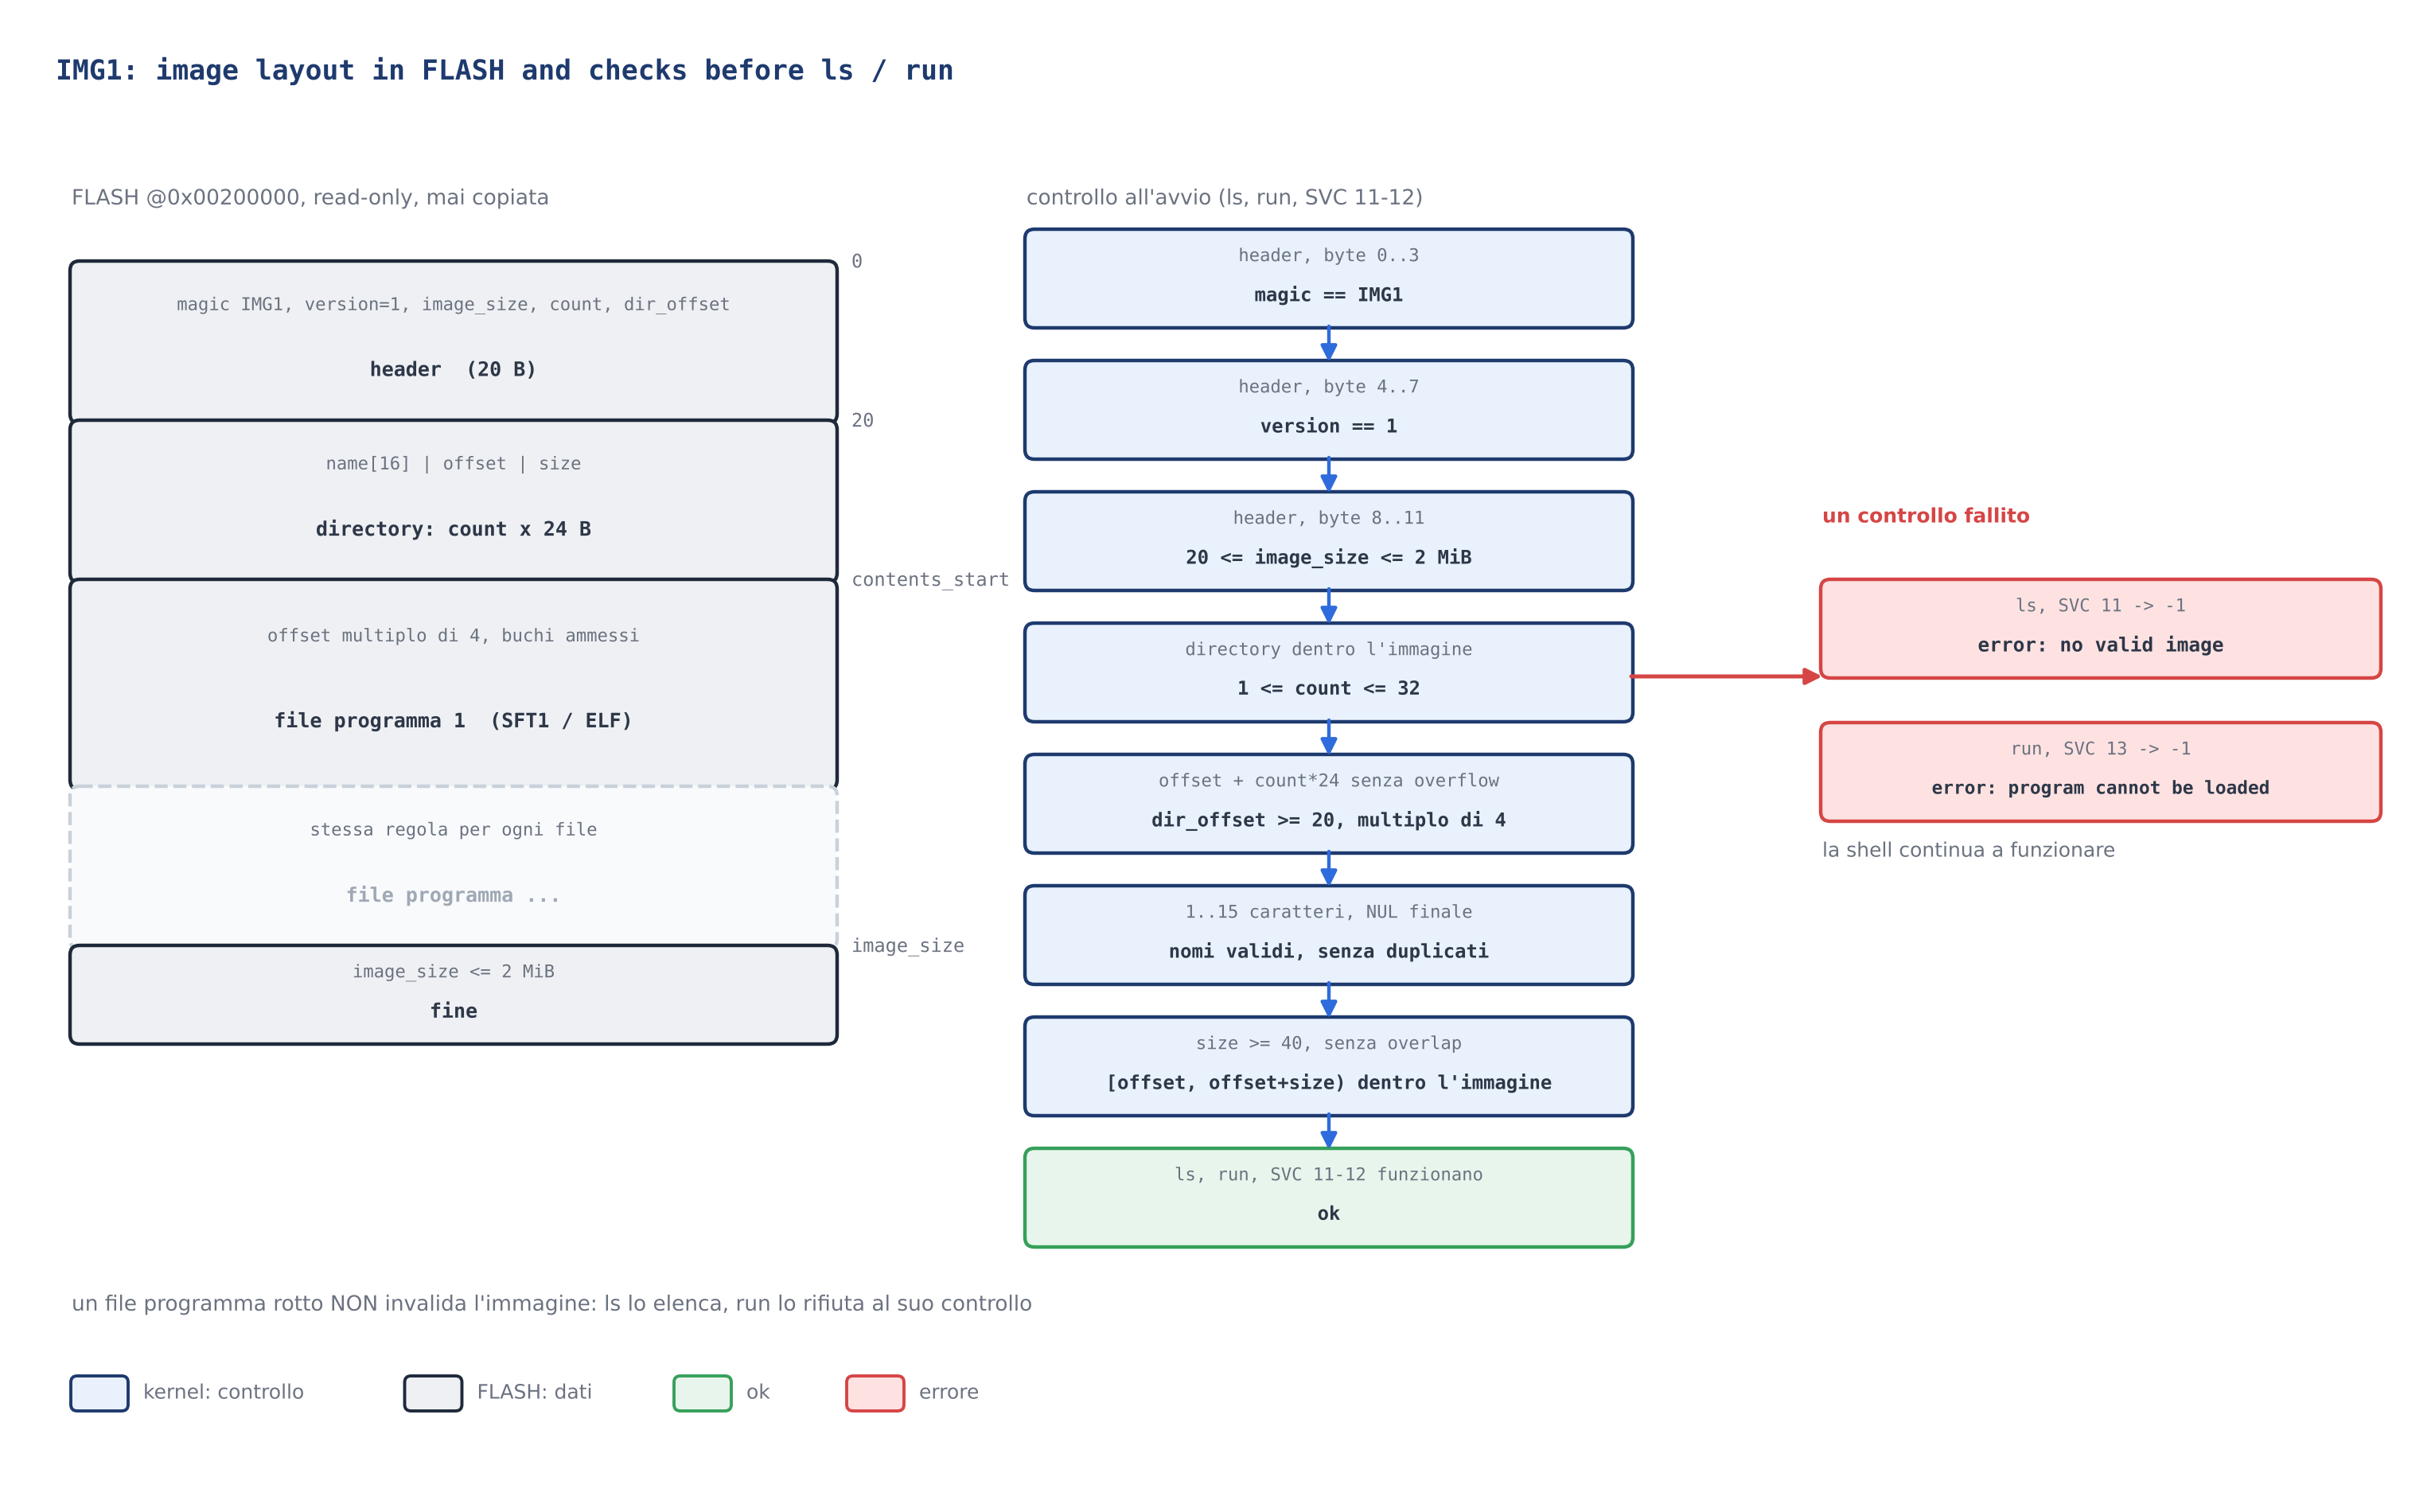
\includegraphics[width=1\textwidth]{contents/images/project/prj_image_format.png}
    \caption{A sinistra il layout dell'immagine IMG1 in FLASH; a destra la catena di controlli che il kernel esegue prima di \texttt{ls} e \texttt{run}. Un controllo fallito rende invalida l'intera immagine, ma non cambia nessuno slot.}
    
\end{figure}

\subsection{Il file programma SFT1 (solo small)}

Le squadre small salvano i programmi in file SFT1. Ogni file inizia con un header di esattamente 40 byte:

\begin{center}
\small
\begin{tabular}{|r|r|l|p{0.45\linewidth}|}
\hline
Byte & Dim. & Campo & \raggedright Valore \tabularnewline
\hline\hline
\texttt{0..3} & 4 & \texttt{magic} & \raggedright magic number di un file SFT1: byte \texttt{53 46 54 31} (\texttt{SFT1}), valore numerico \texttt{0x31544653} \tabularnewline
\hline
\texttt{4..7} & 4 & \texttt{version} & \raggedright esattamente \texttt{1} \tabularnewline
\hline
\texttt{8..11} & 4 & \texttt{header\_size} & \raggedright esattamente 40 \tabularnewline
\hline
\texttt{12..15} & 4 & \texttt{texttt\_size} & \raggedright dimensione di codice e costanti; diversa da zero, multipla di 4 \tabularnewline
\hline
\texttt{16..19} & 4 & \texttt{data\_size} & \raggedright dimensione dei dati inizializzati; multipla di 4 \tabularnewline
\hline
\texttt{20..23} & 4 & \texttt{bss\_size} & \raggedright dimensione del BSS; multipla di 4; questi byte non sono nel file \tabularnewline
\hline
\texttt{24..27} & 4 & \texttt{entry} & \raggedright entry point, contato dall'inizio del codice; il bit 0 vale 1 (Thumb) e \texttt{entry \& \textasciitilde{}1} è minore di \texttt{texttt\_size} \tabularnewline
\hline
\texttt{28..31} & 4 & \texttt{reloc\_offset} & \raggedright inizio della relocation list; multiplo di 4 ed esattamente \texttt{40 + texttt\_size + data\_size} \tabularnewline
\hline
\texttt{32..35} & 4 & \texttt{reloc\_count} & \raggedright numero di voci della relocation list \tabularnewline
\hline
\texttt{36..39} & 4 & \texttt{file\_size} & \raggedright dimensione dell'intero file; uguale alla \texttt{size} della voce di directory e alla fine della relocation list \tabularnewline
\hline
\end{tabular}
\end{center}

\paragraph{Layout.} Codice e costanti occupano \texttt{[40, 40 + texttt\_size)}. I \texttt{data\_size} byte successivi contengono i dati inizializzati. Poi viene la relocation list: \texttt{reloc\_count} parole, ognuna delle quali è l'offset di una parola da correggere. Quindi \texttt{file\_size = reloc\_offset + 4 * reloc\_count}, e dopo la lista non c'è nulla.

\emph{Da chiarire con il professore:} da dove si contano gli offset della relocation list. La regola generale () dice che gli offset si contano dal primo byte del file, e per queste voci il .md non indica eccezioni, mentre per \texttt{entry} dice esplicitamente che si conta dall'inizio del codice. Conviene confermarlo, anche perché eventuali file SFT1 rotti generati dal test kit vanno letti nello stesso modo.

\paragraph{Limiti.} \texttt{texttt\_size + data\_size + bss\_size} non deve andare in overflow e non deve superare 3072 byte. \texttt{reloc\_count} può essere zero ed è al massimo \texttt{(texttt\_size + data\_size) / 4}. Ogni offset di relocation è multiplo di 4, compare una sola volta e indica una parola intera di 4 byte dentro il codice o i dati.

\paragraph{Come lo usa il loader.} Prima di scrivere qualunque cosa nello slot, il loader controlla ogni campo, intervallo, calcolo e relocation, compreso ogni valore \texttt{slot\_base + original\_word}, che non deve andare in overflow sui 32 bit. Poi copia codice e dati, riempie di zeri il BSS e somma la base dello slot a ogni parola elencata. La parola originale può puntare fuori dal programma. Sommare la base mantiene il bit 0 di un puntatore a funzione Thumb.

\paragraph{Errori.} Qualunque errore SFT1 dà il risultato interno \texttt{-4} e il messaggio \texttt{error:\ program cannot be loaded}. Nessun byte del programma viene copiato o eseguito.

\subsection{I file ELF dei programmi e l'host tool}

\paragraph{Com'è fatto ogni ELF.} I programmi sono eseguibili Thumb freestanding per ARM EABI Cortex-M3, non oggetti del kernel. Seguono la normale convenzione di chiamata del C, senza libreria C e senza heap. Ogni ELF è un file ARM a 32 bit, little-endian, versione 1, di tipo \texttt{ET\_EXEC}, linkato all'indirizzo zero con \texttt{--emit-relocs}. I suoi record hanno le dimensioni standard: header del file da 52 byte, program header da 32 byte, section header da 40 byte, simboli da 16 byte e record \texttt{REL} da 8 byte. Almeno un segmento \texttt{PT\_LOAD} descrive la parte da caricare. L'entry point è un indirizzo Thumb dentro il codice. L'ELF non deve contenere record \texttt{RELA}, dynamic linking, simboli non definiti, né tipi di relocation diversi da quelli accettati qui sotto per il contenuto caricato. I dettagli del Makefile li decide la squadra.

\paragraph{Quali relocation contano.} Il campo \texttt{sh\_info} di ogni sezione di relocation dice a quale sezione si applica. Contano solo le relocation delle sezioni caricate in memoria (le sezioni allocated); quelle delle altre sezioni, come le informazioni di debug (compreso \texttt{R\_ARM\_NONE}), si ignorano. Per il contenuto caricato:
\begin{itemize}
\item \texttt{R\_ARM\_ABS32} (un indirizzo completo a 32 bit) va corretta sommando la base dello slot;
\item \texttt{R\_ARM\_THM\_CALL} e \texttt{R\_ARM\_THM\_JUMP24} (salti Thumb) sono relative alla posizione corrente: si controllano ma non si modificano;
\item ogni altro tipo viene rifiutato.
\end{itemize}

\paragraph{Small: conversione da ELF a SFT1.} Il converter legge header ELF da 52 byte, program header da 32 byte e section header da 40 byte. Tutte le tabelle devono essere valide e stare dentro il file, e deve esserci almeno un \texttt{PT\_LOAD}. L'indirizzo di caricamento più basso e il contenuto caricato partono da zero. Le sezioni caricate non si sovrappongono e stanno dentro i segmenti caricabili. Le sezioni con contenuto iniziale vengono prima di tutte le sezioni \texttt{SHT\_NOBITS} (BSS), e le sezioni read-only prima di quelle scrivibili.

Il converter riempie di zeri i buchi e il padding di allineamento, arrotonda a un multiplo di 4 la fine del codice, dei dati inizializzati e della memoria totale, e rifiuta i programmi più grandi di 3072 byte. Accetta solo record \texttt{REL} validi che usano simboli definiti. I site \texttt{R\_ARM\_ABS32} allineati a parola diventano la relocation list SFT1, ordinata e senza duplicati. I site \texttt{R\_ARM\_THM\_CALL} e \texttt{R\_ARM\_THM\_JUMP24} allineati a mezza parola si controllano e non producono voci. Il converter rifiuta \texttt{RELA}, relocation nel BSS, simboli non definiti, site non validi e ogni altro tipo di relocation per il contenuto caricato.

\paragraph{Small: comandi dell'host tool.} I comandi sono esattamente:
\begin{lstlisting}[language=bash]
python3 tools/mkimage.py flat PROGRAM.elf PROGRAM.sft
python3 tools/mkimage.py image build/fs.img NAME=PROGRAM.elf [NAME=PROGRAM.elf ...]
\end{lstlisting}
\begin{sloppypar}
In caso di successo \texttt{flat} stampa \texttt{SFT1:\ ELF -> OUTPUT (N bytes)} e \texttt{image} stampa \texttt{IMG1:\ OUTPUT (N bytes, C programs)}. Nella small \texttt{image} riceve file ELF, ma il kernel small legge solo SFT1: nell'immagine finiscono quindi i programmi convertiti in SFT1.
\end{sloppypar}

Prima di scrivere qualunque output, lo strumento rifiuta argomenti, nomi e file ELF sbagliati e risultati troppo grandi. Gli errori passano da \texttt{argparse} di Python, che scrive \texttt{mkimage.py:\ error:\ <reason>} su standard error ed esce con stato 2.

\paragraph{Big: comando dell'host tool.} Il comando è esattamente:
\begin{lstlisting}[language=bash]
python3 tools/mkimage.py image build/fs.img NAME=PROGRAM.elf [NAME=PROGRAM.elf ...]
\end{lstlisting}
Valgono tutte le regole IMG1. Lo strumento copia ogni ELF byte per byte, senza modifiche. Le squadre big non hanno bisogno del comando \texttt{flat}.

\begin{sloppypar}
\paragraph{Big: che cosa controlla il kernel in un ELF.} Il kernel controlla l'identità dell'ELF, le dimensioni dei record e ogni tabella di program header o di sezioni che usa. Controlla i segmenti caricabili e le sezioni caricate che gli servono per trovare i target delle relocation, tutte le sezioni \texttt{REL} e i simboli usati dalle relocation che contano. Prima di usare un valore, verifica che ogni calcolo, tabella, record, segmento, sezione, site di relocation e intervallo copiato stia dentro il file e dentro lo slot. Non deve controllare i nomi delle sezioni, il contenuto di debug o delle stringhe, né i campi dei simboli che non usa.
\end{sloppypar}

Per le sezioni caricate applica \texttt{R\_ARM\_ABS32} sommando la base dello slot e accetta senza modifiche \texttt{R\_ARM\_THM\_CALL} e \texttt{R\_ARM\_THM\_JUMP24} risolte. Ignora le relocation delle altre sezioni, purché i loro record stiano dentro il file. Per qualunque altro tipo in una sezione caricata stampa prima la riga
\begin{lstlisting}
loader: unsupported relocation type <type>
\end{lstlisting}
con il tipo come numero decimale, e poi il normale messaggio di rifiuto. Un ELF malformato viene rifiutato senza fault del kernel.

\subsection{Mappa di memoria e slot}

Si usa la mappa di memoria completa del linker script della base:

\begin{center}
\small
\begin{tabular}{|p{0.42\linewidth}|p{0.42\linewidth}|}
\hline
\raggedright Area & \raggedright Indirizzi \tabularnewline
\hline\hline
\raggedright FLASH della board (4 MiB), usata dal kernel & \raggedright da \texttt{0x00000000} \tabularnewline
\hline
\raggedright Immagine \texttt{fs.img} & \raggedright da \texttt{0x00200000}, mai oltre \texttt{0x00400000} \tabularnewline
\hline
\raggedright Partizione RAM della shell & \raggedright \texttt{0x20000000..0x20000fff} \tabularnewline
\hline
\raggedright Partizione dell'idle task & \raggedright \texttt{0x20001000..0x20001fff} \tabularnewline
\hline
\raggedright Slot 0 & \raggedright \texttt{0x20002000..0x20002fff} \tabularnewline
\hline
\raggedright Slot 1 & \raggedright \texttt{0x20003000..0x20003fff} \tabularnewline
\hline
\raggedright Slot 2 & \raggedright \texttt{0x20004000..0x20004fff} \tabularnewline
\hline
\raggedright Slot 3 & \raggedright \texttt{0x20005000..0x20005fff} \tabularnewline
\hline
\end{tabular}
\end{center}

Dati e stack del kernel stanno fuori dalle partizioni di shell e idle task. Gli slot sono quattro, fissi, da 4096 byte, ciascuno allineato a 4096 byte.

\paragraph{Scelta dello slot.} Il loader prende sempre il primo slot libero, nell'ordine 0, 1, 2, 3.

\paragraph{Dentro uno slot.} Codice, dati, BSS e stack condividono lo slot:

\begin{center}
\small
\begin{tabular}{|l|p{0.6\linewidth}|}
\hline
Offset nello slot & \raggedright Contenuto \tabularnewline
\hline\hline
da 0 a 3071 & \raggedright il programma (codice + dati + BSS), che usa al massimo i 3072 byte bassi \tabularnewline
\hline
da 3072 a 4095 & \raggedright lo stack (1024 byte), che cresce verso il basso; i frame iniziali preparati dal codice dato usano i 64 byte in cima \tabularnewline
\hline
\end{tabular}
\end{center}

Lo stack pointer iniziale è la fine dello slot.

\paragraph{Esecuzione e protezione.} I programmi girano unprivileged in Thread mode, sul process stack (PSP), sotto lo scheduler round-robin preemptive già esistente. Non devono accedere alla RAM del kernel né ad altri slot. Come nel setup MPU della base, la FLASH \texttt{0x00000000..0x003fffff} si può leggere ed eseguire da ogni task unprivileged: serve alla shell, che ha il codice in FLASH, mentre un programma caricato esegue solo la copia nel suo slot.
\begin{itemize}
\item Small: una regione MPU dà lettura, scrittura ed esecuzione sullo slot corrente.
\item Big: le regioni danno al codice lettura ed esecuzione, senza scrittura, e a dati e stack lettura e scrittura, senza esecuzione (W\textasciicircum{}X).
\end{itemize}

\begin{figure}[H]
    \centering
    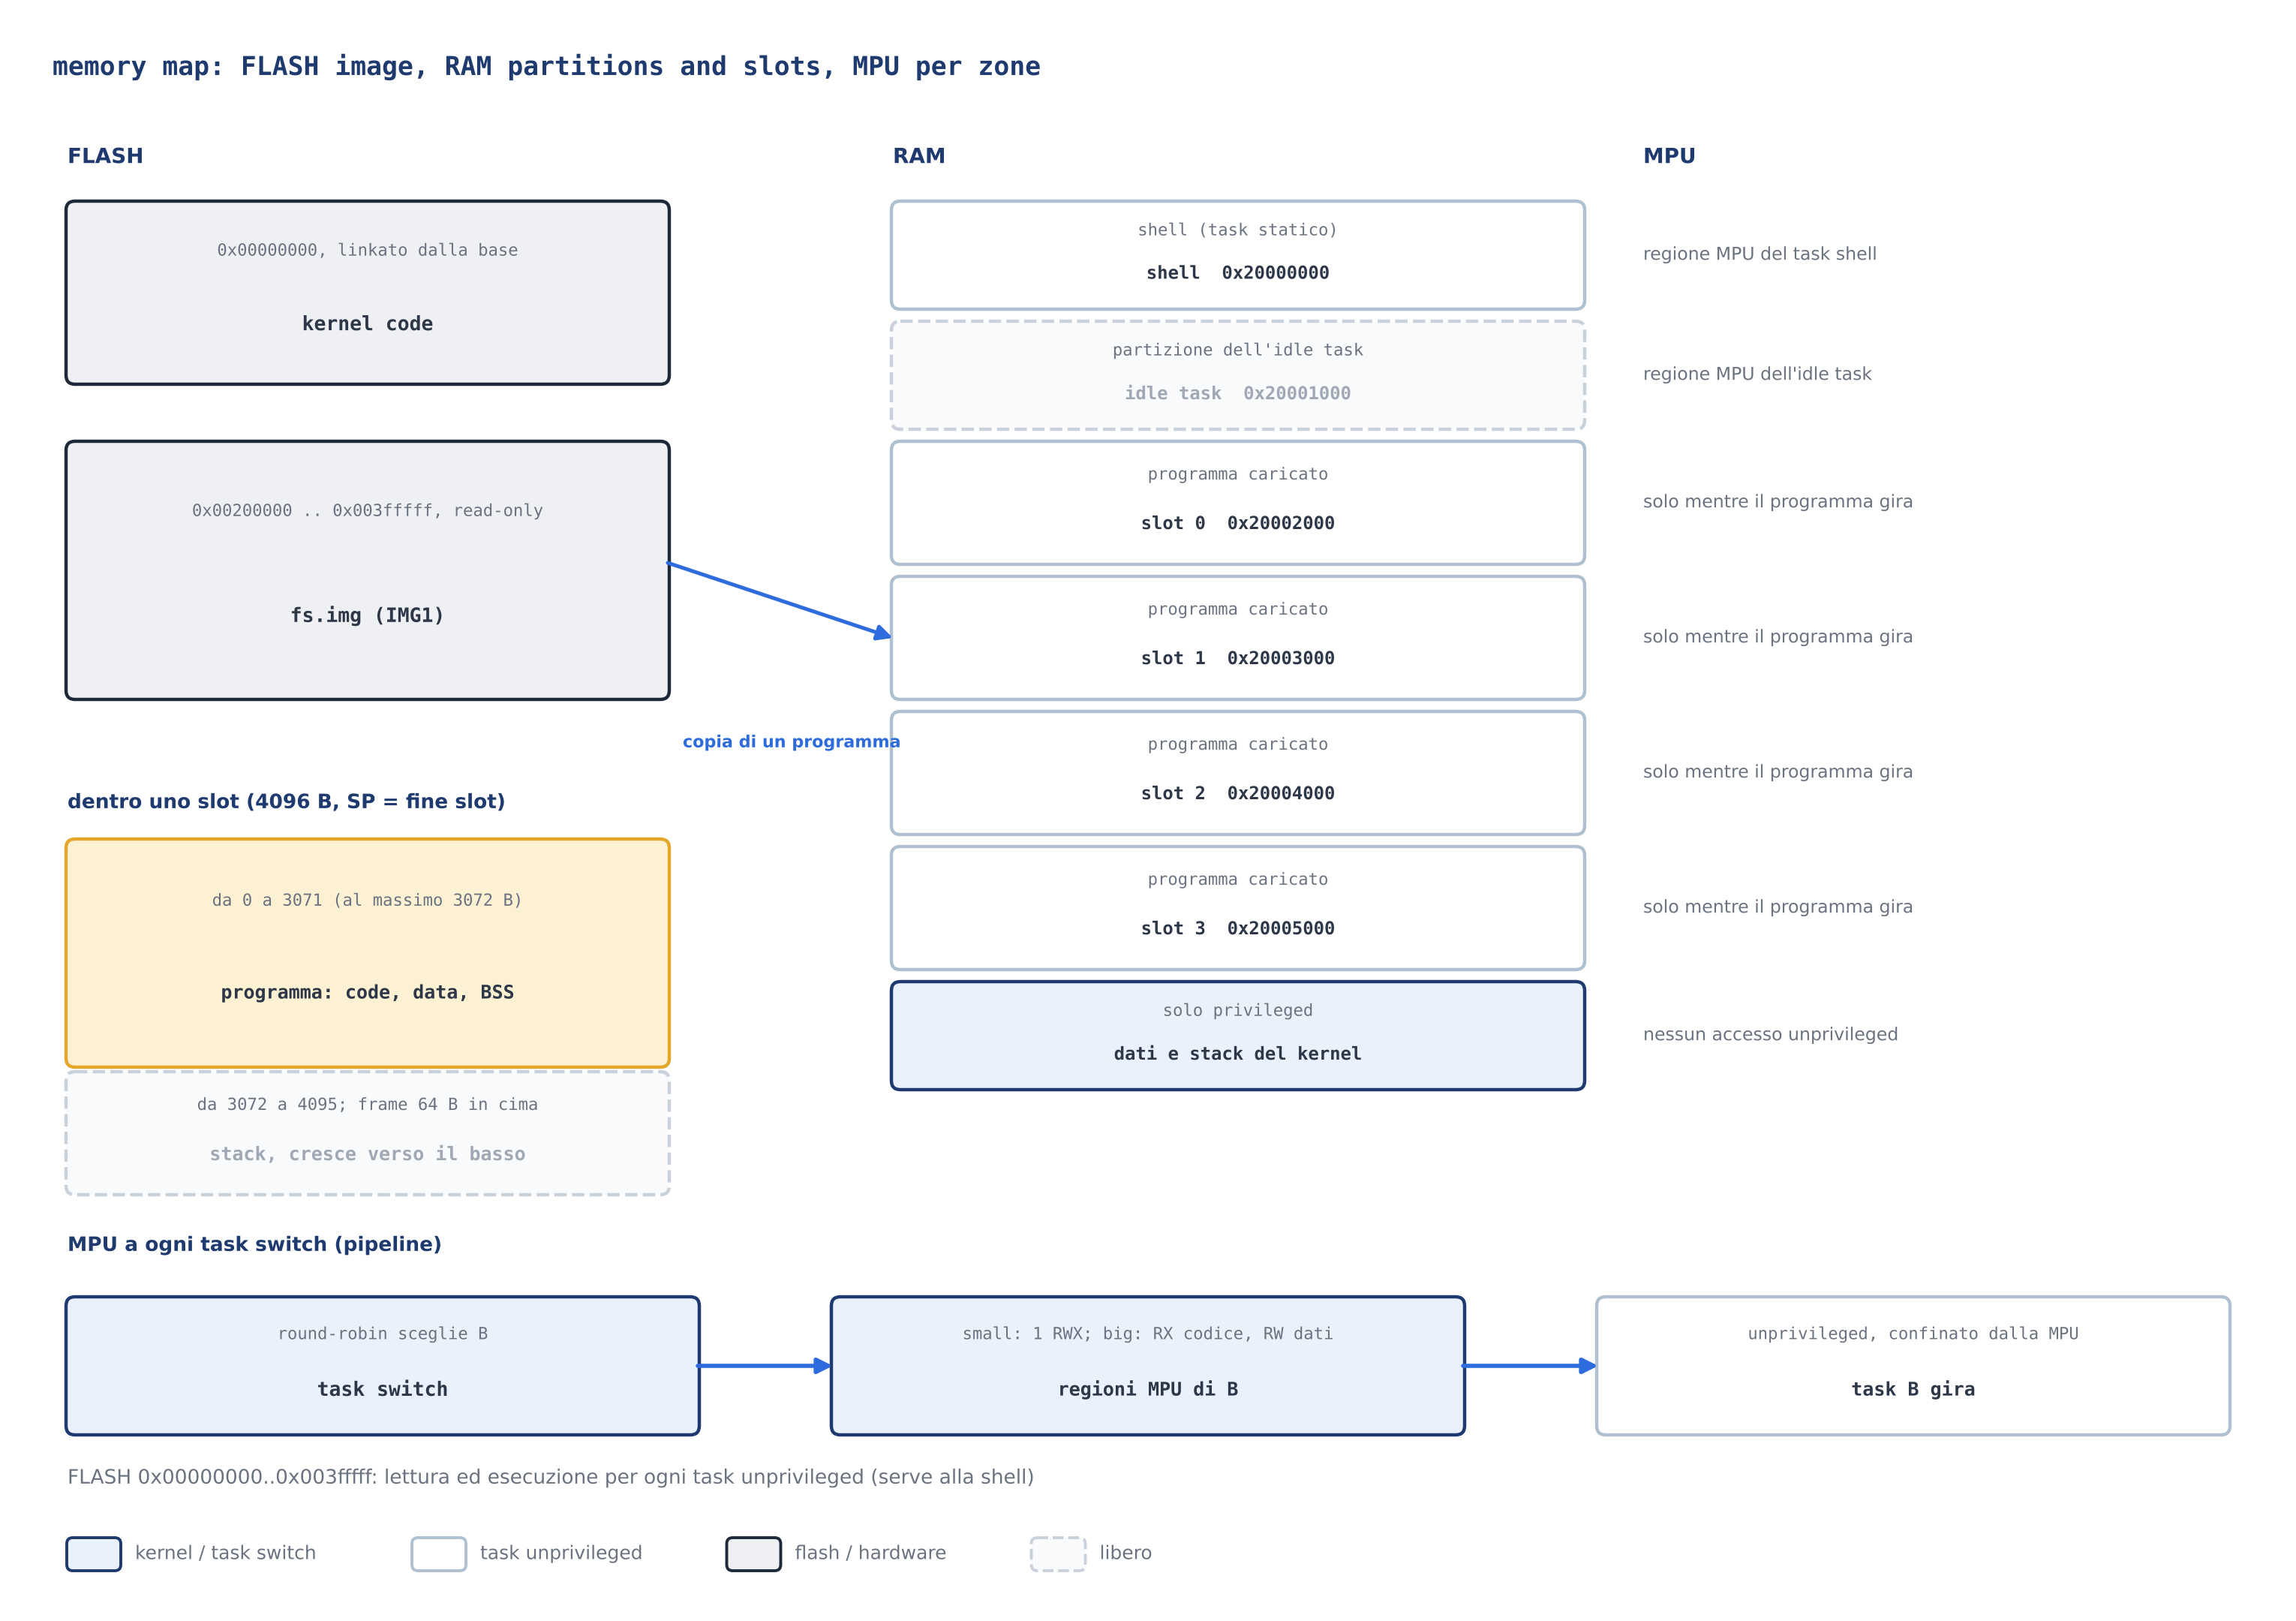
\includegraphics[width=1\textwidth]{contents/images/project/prj_memory_map.png}
    \caption{Mappa di memoria: FLASH con kernel e immagine, RAM con partizioni, slot e dati del kernel, e a destra la regione MPU di ciascuna zona. In uno slot il programma usa i primi 3072 byte, lo stack i restanti 1024; a ogni task switch la MPU viene riprogrammata.}
    
\end{figure}

\subsection{System call}

\begin{sloppypar}
\paragraph{Chiamate già esistenti.} I programmi possono linkare gli stub di \texttt{lib/syscalls.s}. I prototipi sono:
\end{sloppypar}
\begin{lstlisting}[language=C]
int sys_write(const char *buf, unsigned len);
int sys_read(void);
uint32_t sys_uptime(void);
void sys_exit(void);
void task_yield(void);
void task_delay(uint32_t ticks);
int task_delay_until(uint32_t *last_wake,
                     uint32_t period);
void trace_dump(void);
uint32_t task_tick_count(void);
\end{lstlisting}

\begin{center}
\small
\begin{tabular}{|r|p{0.25\linewidth}|p{0.52\linewidth}|}
\hline
SVC & \raggedright Funzione & \raggedright Risultato \tabularnewline
\hline\hline
1 & \raggedright \texttt{sys\_write} & \raggedright numero di byte accettati, \texttt{0..len}; \texttt{-1} se l'intervallo di byte non sta tutto nella partizione del chiamante o in FLASH \tabularnewline
\hline
2 & \raggedright \texttt{sys\_read} & \raggedright prossimo byte della UART, \texttt{0..255}, oppure \texttt{-1} se non c'è nessun byte in attesa \tabularnewline
\hline
3 & \raggedright \texttt{sys\_uptime} & \raggedright millisecondi dall'avvio del clock \tabularnewline
\hline
4 & \raggedright \texttt{sys\_exit} & \raggedright non ritorna; per i programmi caricati vedi sotto \tabularnewline
\hline
5 & \raggedright servizio di avvio, solo kernel & \raggedright un task riceve \texttt{-1} \tabularnewline
\hline
6 & \raggedright \texttt{task\_yield} & \raggedright chiede un task switch; il chiamante resta pronto a girare \tabularnewline
\hline
7 & \raggedright \texttt{task\_delay} & \raggedright blocca per il numero indicato di tick da 10 ms; zero equivale a una yield \tabularnewline
\hline
8 & \raggedright \texttt{task\_delay\_until} & \raggedright \texttt{0}; \texttt{-1} se la destinazione allineata di 4 byte non sta tutta nella partizione del chiamante \tabularnewline
\hline
9 & \raggedright \texttt{trace\_dump} & \raggedright stampa la trace esistente dello scheduler \tabularnewline
\hline
10 & \raggedright \texttt{task\_tick\_count} & \raggedright tick dall'avvio dello scheduler \tabularnewline
\hline
\end{tabular}
\end{center}

La \texttt{lib/printf.h} fornita supporta \texttt{\%c}, \texttt{\%s}, \texttt{\%d}, \texttt{\%u}, \texttt{\%x} e \texttt{\%\%}, e restituisce il numero di caratteri stampati.

\paragraph{Nuove chiamate del loader.} Gli argomenti passano nei registri \texttt{r0}, \texttt{r1} e \texttt{r2} del chiamante e il risultato torna in \texttt{r0}. Ogni intervallo di memoria che appartiene al chiamante deve stare tutto nella sua partizione.
\begin{lstlisting}[language=C]
int sys_image_count(void);
int sys_image_name(unsigned index, char *name,
                   unsigned capacity);
int sys_program_run(const char *name);
int sys_program_wait(int task_id);
\end{lstlisting}

\begin{center}
\small
\begin{tabular}{|r|p{0.27\linewidth}|p{0.52\linewidth}|}
\hline
SVC & \raggedright Nome & \raggedright Risultato \tabularnewline
\hline\hline
11 & \raggedright \texttt{SYS\_IMAGE\_COUNT}\newline\texttt{sys\_image\_count} & \raggedright numero di voci della directory, \texttt{1..32}; \texttt{-1} se l'immagine non è valida \tabularnewline
\hline
12 & \raggedright \texttt{SYS\_IMAGE\_NAME}\newline\texttt{sys\_image\_name} & \raggedright copia il nome completo, con il NUL finale, e restituisce \texttt{0}; \texttt{-1} se l'immagine o l'indice non sono validi, se \texttt{capacity} non è in \texttt{1..16}, se la destinazione è fuori dalla partizione del chiamante o se il nome non ci sta \tabularnewline
\hline
13 & \raggedright \texttt{SYS\_PROGRAM\_RUN}\newline\texttt{sys\_program\_run} & \raggedright il task id (un numero non negativo); \texttt{-1} per un puntatore o una stringa del nome non validi o per un'immagine non valida; \texttt{-2} se il programma non c'è; \texttt{-3} se nessuno slot è libero; \texttt{-4} se il file programma non è valido \tabularnewline
\hline
14 & \raggedright \texttt{SYS\_PROGRAM\_WAIT}\newline\texttt{sys\_program\_wait} & \raggedright aspetta la fine di quel programma, oppure restituisce subito lo stato salvato quando è finito: \texttt{0} dopo return o exit, \texttt{-2} dopo un fault recuperato; \texttt{-1} per zero, per l'id del chiamante stesso o per un id malformato, sconosciuto o vecchio \tabularnewline
\hline
\end{tabular}
\end{center}

Altri dettagli:
\begin{itemize}
\item \emph{SVC 12.} La FLASH non è una destinazione valida. Se \texttt{capacity} è troppo piccola, la chiamata copia la prima parte del nome, comunque terminata da NUL, e restituisce \texttt{-1}.
\item \emph{SVC 13.} \texttt{name} deve essere non vuoto e terminare con NUL entro 16 byte, quindi ha al massimo 15 caratteri. Ogni byte letto deve stare nella partizione del chiamante o in FLASH \texttt{0x00000000..0x003fffff}. I caratteri non vengono confrontati con le regole dei nomi: un nome che non può esistere restituisce semplicemente \texttt{-2}.
\item \emph{SVC 14.} Non c'è un puntatore di output: quando il programma finisce, il risultato viene scritto nel valore di \texttt{r0} salvato del chiamante in attesa. Un task id contiene il numero dello slot nei bit 1:0 e, sopra, un contatore di generation a 28 bit diverso da zero: i primi id sono 4, 5, 6 e 7 per gli slot 0, 1, 2 e 3, e il programma successivo nello slot 0 riceve l'id 8 (in pratica $\mathit{id} = 4 \cdot \mathit{generation} + \mathit{slot}$). Ogni slot conserva uno stato di fine finché non termina il suo programma successivo. Aspettare non riserva uno slot liberato. Più task possono aspettare lo stesso programma in esecuzione.
\item \emph{SVC 4.} Non ha argomenti e non ritorna. Per un programma caricato equivale a tornare da \texttt{main}: stampa il messaggio di uscita, salva lo stato 0, sveglia i task in attesa, libera lo slot e passa a un altro task. Per un task statico termina il task, senza messaggio di programma e senza uno slot riusabile.
\item \emph{Chiamate sconosciute.} I numeri di SVC sconosciuti, la SVC 0 e un task che chiama la SVC 5 (riservata al kernel) ricevono \texttt{-1}.
\item \emph{SVC 1 con lunghezza 0.} Restituisce 0 senza leggere memoria se il puntatore è dentro la partizione del chiamante o la FLASH, o esattamente sul loro bordo; qualunque altro puntatore dà \texttt{-1}. I calcoli sugli intervalli non devono andare in overflow.
\end{itemize}

\begin{figure}[H]
    \centering
    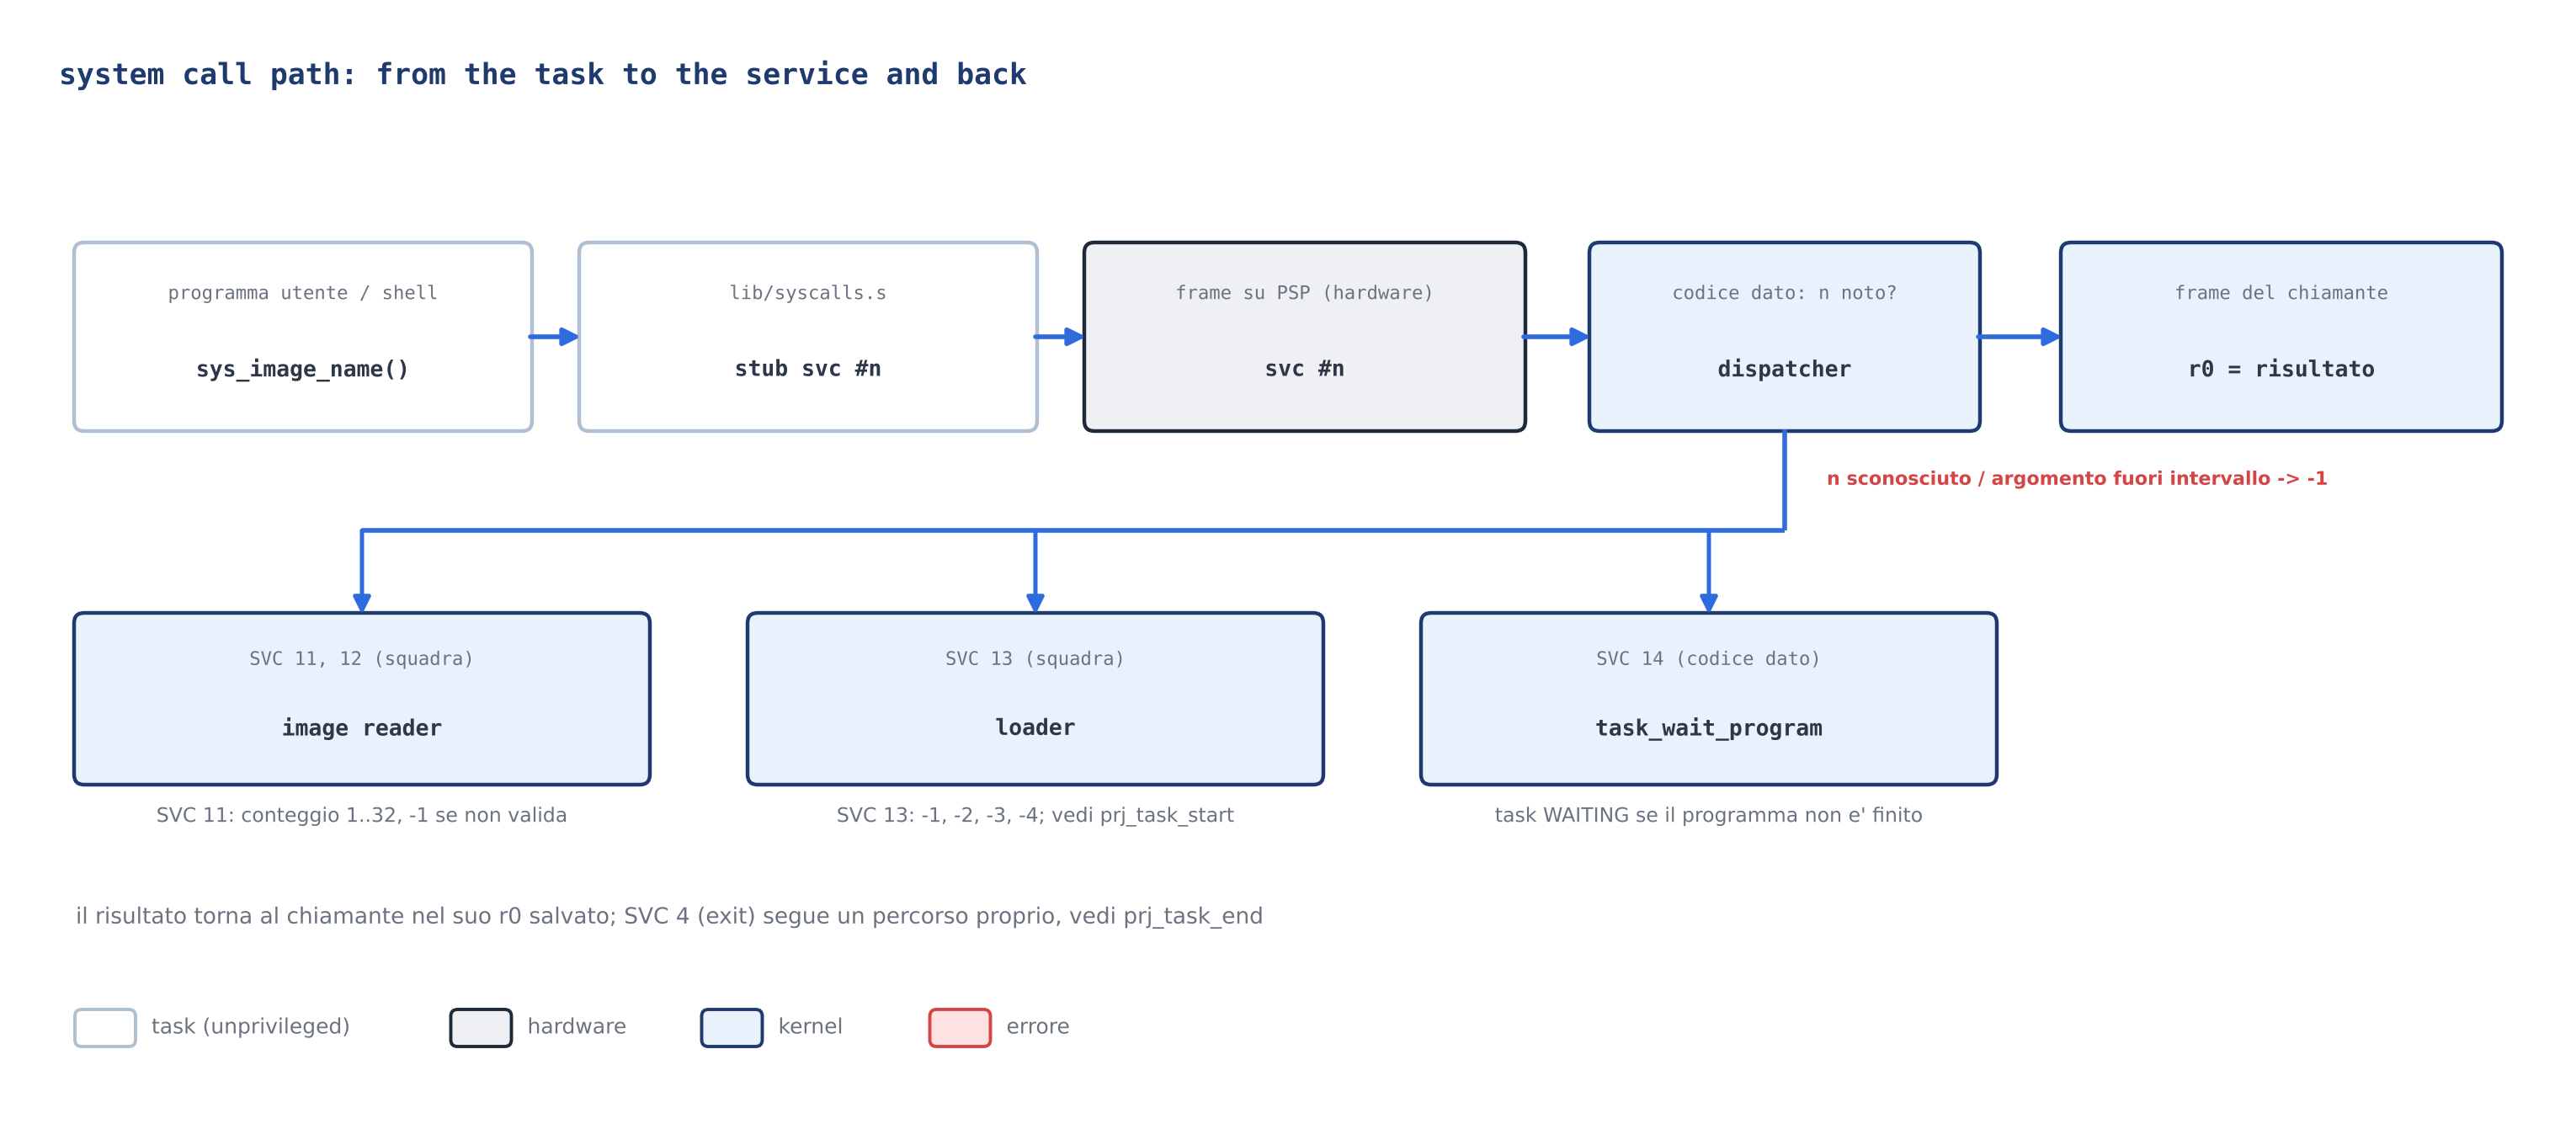
\includegraphics[width=1\textwidth]{contents/images/project/prj_syscall_path.png}
    \caption{Percorso di una system call: lo stub in \texttt{lib/syscalls.s} esegue \texttt{svc \#n}, il dispatcher controlla numero e argomenti, e il risultato torna in \texttt{r0} del chiamante. Le SVC 11, 12 e 13 sono servizi del progetto; la SVC 14 è già data.}
    
\end{figure}

\subsection{Input e output della shell}

\paragraph{All'avvio.} Il kernel stampa:
\begin{lstlisting}
scratch-os: kernel started
scheduler: round robin, quantum 5 ticks
\end{lstlisting}

\paragraph{Lettura di una riga.} La shell stampa il prompt \texttt{scratch> }, con uno spazio finale e senza andare a capo. Fa l'eco di ogni carattere memorizzato, senza cambiarlo. Un CR o un LF stampa un solo a capo e chiude la riga. La shell memorizza e ripete in eco al massimo 31 caratteri: quelli in più vengono scartati, senza eco, fino alla fine della riga. Non c'è line editing e gli spazi non vengono tolti.

\paragraph{Comandi.} Gli unici comandi sono esattamente \texttt{help}, \texttt{ls} e \texttt{run } seguito da un nome non vuoto. Un secondo spazio dopo \texttt{run } fa parte del nome. Una riga vuota, \texttt{run} da solo, caratteri in più dopo \texttt{help} o \texttt{ls}, e qualunque altro input stampano \texttt{error:\ unknown command}.

\texttt{help} stampa esattamente:
\begin{lstlisting}
help - show commands
ls - list programs
run <name> - run a program
\end{lstlisting}

\texttt{ls} stampa i nomi dei programmi nell'ordine della directory, uno per riga. Se l'immagine non è valida stampa:
\begin{lstlisting}
error: no valid image
\end{lstlisting}

Quando \texttt{run <name>} fallisce, la shell stampa, rispettivamente per i risultati \texttt{-2}, \texttt{-3} e per qualunque altro valore negativo:
\begin{lstlisting}
error: program not found
error: no free slot
error: program cannot be loaded
\end{lstlisting}

Quando \texttt{run <name>} riesce, il kernel stampa la riga seguente, con numeri esadecimali minuscoli e senza zeri iniziali. A stamparla è la funzione data \texttt{task\_program\_create}:
\begin{lstlisting}
loader: <name> slot=<slot> base=0x<base> id=<id>
\end{lstlisting}

Mentre il programma gira, la shell aspetta e non stampa il prompt. Quando il programma torna da \texttt{main} o chiama la SVC 4, il sistema stampa:
\begin{lstlisting}
program <name> exited
\end{lstlisting}

Quando un programma caricato provoca un fault recuperabile, il sistema stampa:
\begin{lstlisting}
<kind> in loaded program: CFSR=0x<cfsr>[ address=0x<mmfar>]
program <name> faulted
\end{lstlisting}
\texttt{<kind>} è esattamente \texttt{MemManage}, \texttt{BusFault}, \texttt{UsageFault} o \texttt{HardFault}. La parte tra parentesi quadre compare solo quando è attivo il bit \texttt{MMARVALID}. La wait restituisce \texttt{-2}, lo slot viene liberato e il prompt ricompare.

Alcuni fault non sono recuperabili: un MemManage o un BusFault che avviene mentre il processore salva o ripristina lo stack frame, un HardFault causato da un errore di stack di questo tipo, e qualunque fault fuori da un programma caricato. In questi casi il sistema stampa la riga seguente e si ferma, senza un altro prompt:
\begin{lstlisting}
<kind>: unrecoverable CFSR=0x<cfsr> HFSR=0x<hfsr>
\end{lstlisting}

Il prompt ricompare dopo ogni altro comando, ogni caricamento fallito e ogni fault recuperato. Comandi extra o output di debug non devono mai comparire in queste trascrizioni, né ritardarle o cambiarle.

\paragraph{Due conseguenze delle regole.}
\begin{itemize}
\item Sulla riga stanno 31 caratteri, quindi dopo \texttt{run } un nome può arrivare a 27 caratteri, ma la SVC 13 ne accetta al massimo 15. Con un nome più lungo la SVC 13 restituisce \texttt{-1} e la shell stampa \texttt{error:\ program cannot be loaded}, non \texttt{error:\ program not found}.
\item Con due spazi dopo \texttt{run} il nome cercato inizia con uno spazio, quindi non esiste: la SVC 13 restituisce \texttt{-2} e la shell stampa \texttt{error:\ program not found}.
\end{itemize}

\begin{figure}[H]
    \centering
    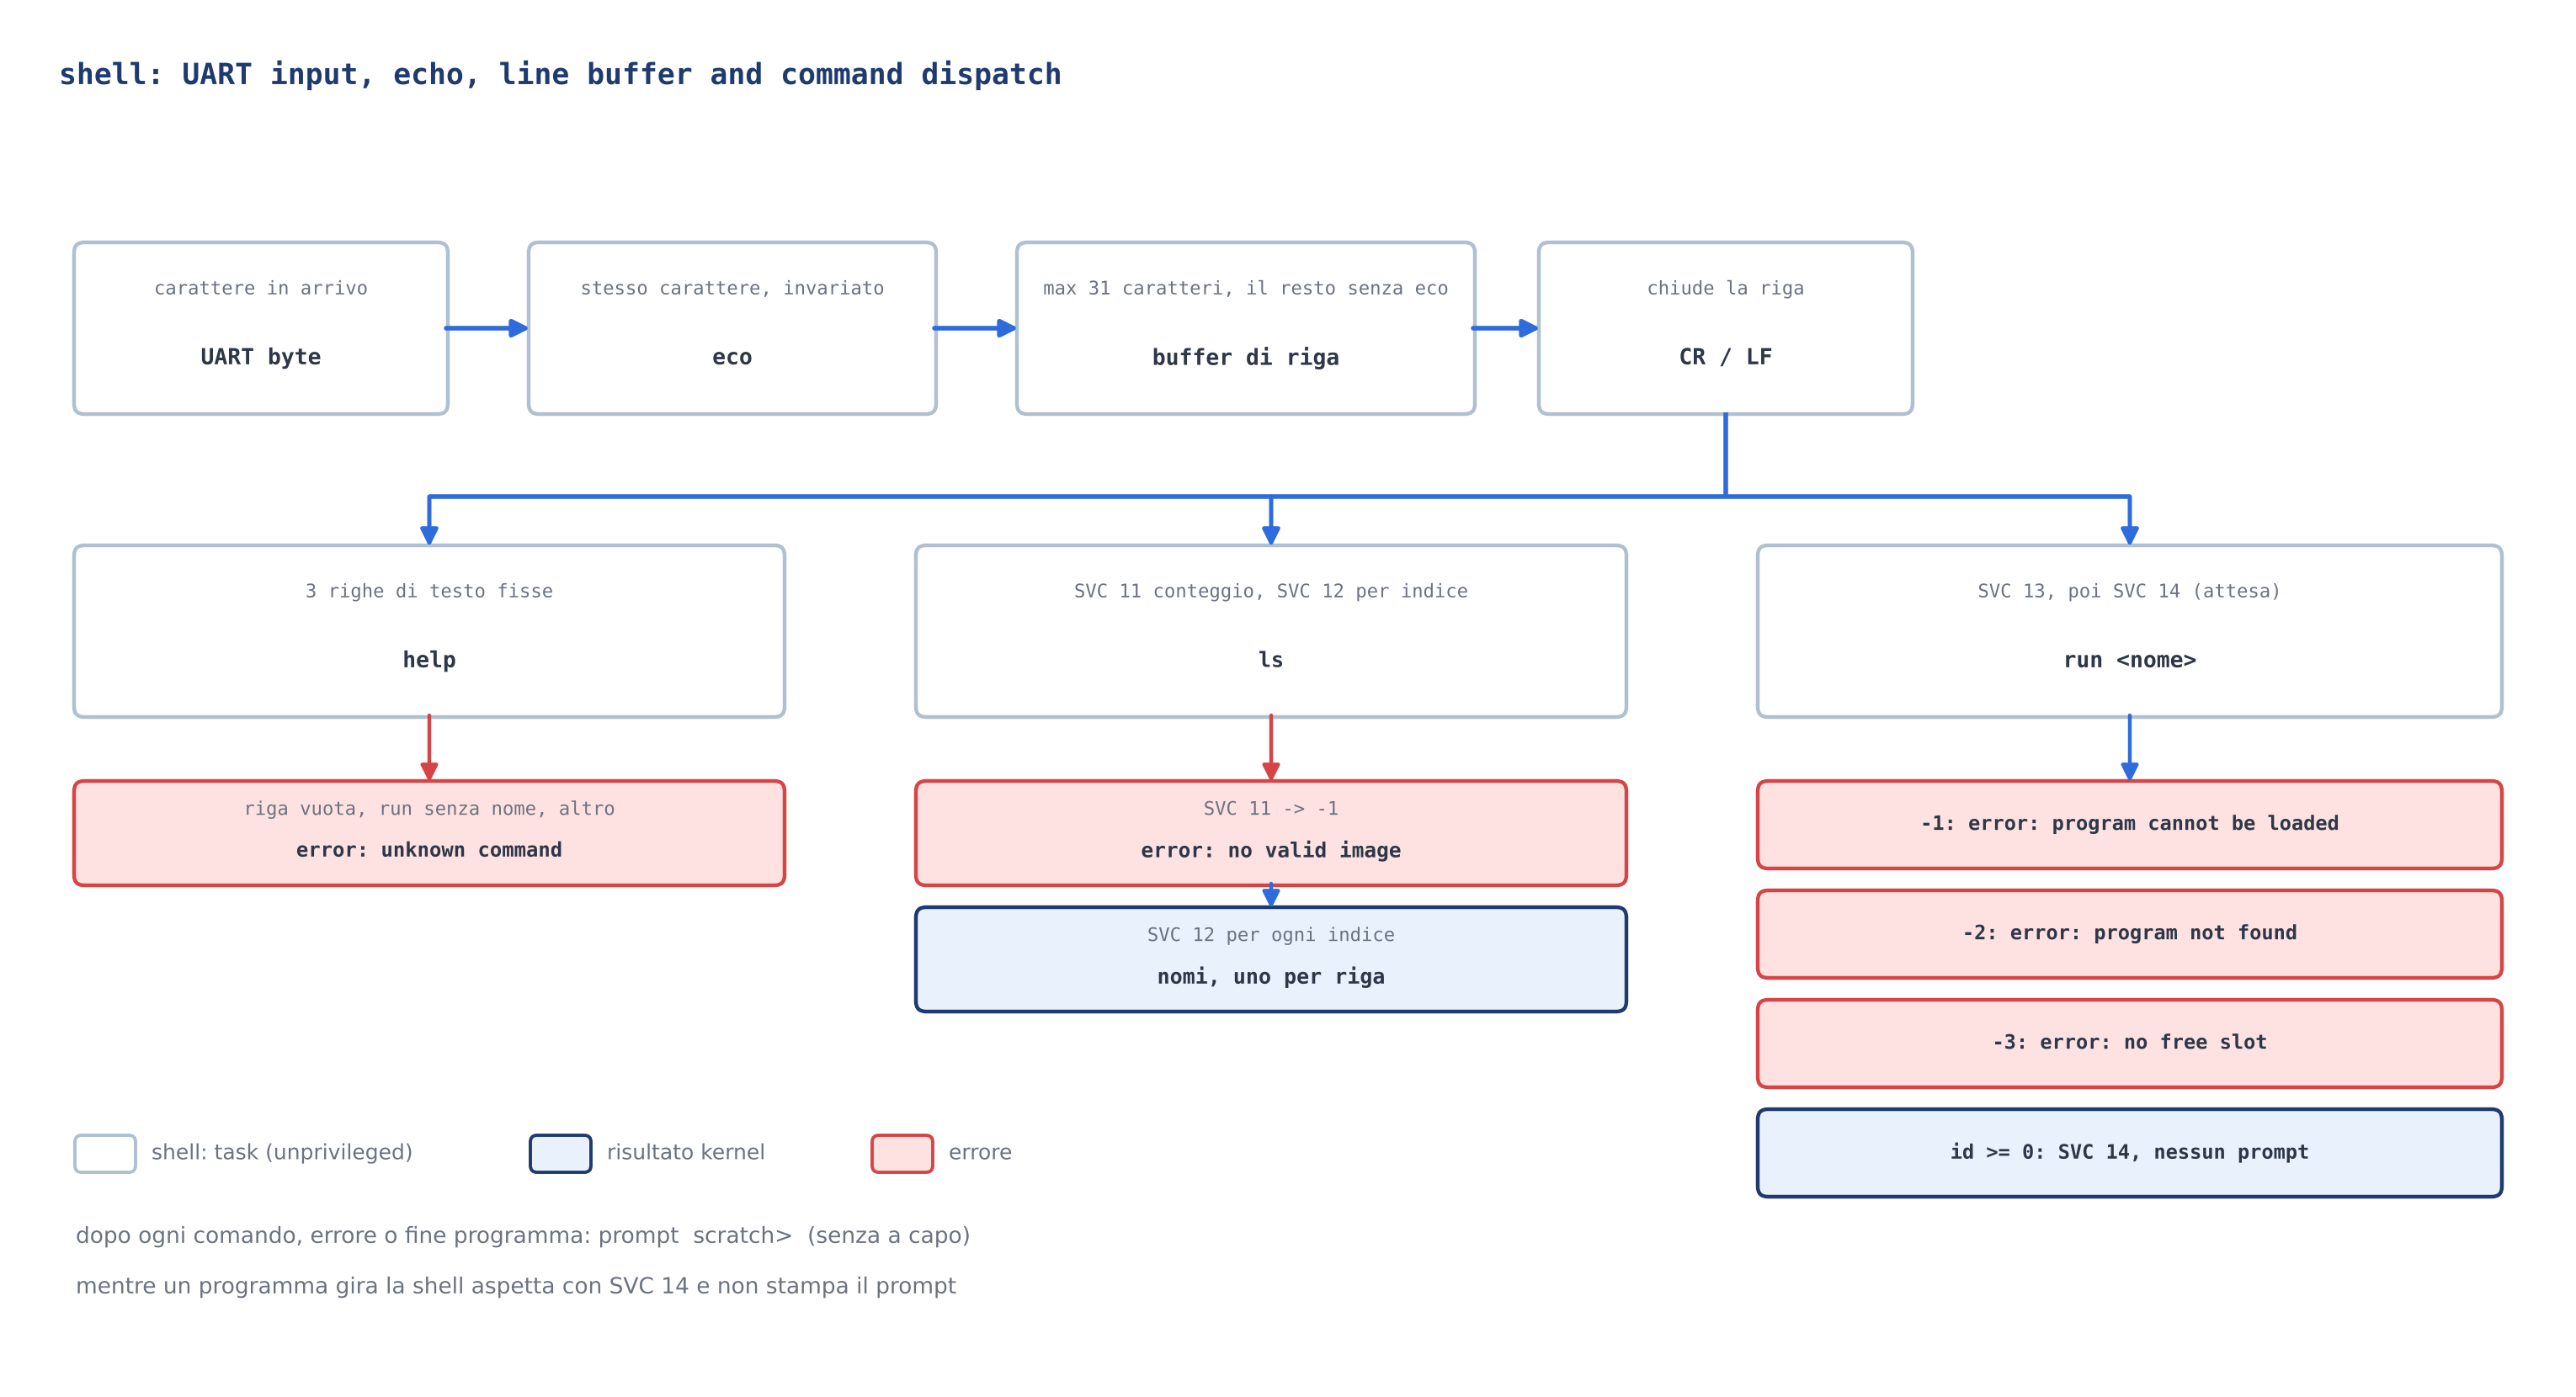
\includegraphics[width=1\textwidth]{contents/images/project/prj_shell.png}
    \caption{Percorso dell'input della shell: ogni carattere viene ripetuto in eco, la riga si chiude con CR o LF e il comando decide quali system call usare. Dopo ogni esito la shell torna al prompt, tranne mentre un programma gira.}
    
\end{figure}

\subsection{Il codice dato da usare}

La base contiene già quattro task record (TCB) riusabili per i programmi caricati, i task id con il contatore di generation, i record di attesa e di stato di fine, e gli stack frame iniziali. Gestisce anche return, exit e fault recuperati, sveglia i task in attesa e implementa la SVC 14. Questo codice non va sostituito né copiato.

\begin{sloppypar}
Il codice della squadra fornisce la shell tramite \texttt{task\_project\_configure()} e \texttt{task\_configure\_shell()}. Fornisce anche le SVC da 11 a 13, i controlli sui file, il caricamento, la relocation, i controlli di entry e stack e i permessi MPU. La funzione data \texttt{task\_program\_create} si chiama solo dopo che il programma è stato caricato per intero e senza errori.
\end{sloppypar}

L'interfaccia è dichiarata in \texttt{kernel/task.h}:
\begin{lstlisting}[language=C]
task_project_configure(void)
task_configure_shell(name, entry, stack_top,
                     part_start, part_end,
                     data_start, data_end, data_load)
task_program_slot_free(slot)
task_program_create(slot, name, entry, stack_top,
                    executable)
task_wait_program(id, saved_result)
\end{lstlisting}

\begin{center}
\small
\begin{tabular}{|p{0.36\linewidth}|p{0.52\linewidth}|}
\hline
\raggedright Funzione & \raggedright Che cosa fa e come si usa \tabularnewline
\hline\hline
\raggedright \texttt{task\_project\_configure} & \raggedright hook weak della base: la squadra ne scrive una definizione normale (strong) e lì configura la shell \tabularnewline
\hline
\raggedright \texttt{task\_configure\_shell} & \raggedright imposta il task della shell; si passano gli indirizzi dei simboli del linker della shell corrispondenti \tabularnewline
\hline
\raggedright \texttt{task\_program\_slot\_free} & \raggedright dice se uno slot è libero; è falsa per uno slot occupato o inesistente \tabularnewline
\hline
\raggedright \texttt{task\_program\_create} & \raggedright crea il task e restituisce il suo id, oppure \texttt{-1}; copia al massimo 15 caratteri del nome, costruisce i frame iniziali da 64 byte, mette il task in READY e stampa la riga \texttt{loader:} esatta \tabularnewline
\hline
\raggedright \texttt{task\_wait\_program} e codice della SVC 14 & \raggedright supporto per l'attesa e lo stato di fine; non si aggiunge un altro modo di aspettare attraverso il suo helper del kernel \tabularnewline
\hline
\raggedright \texttt{task\_finish\_current}, \texttt{task\_fault\_current}, \texttt{task\_current\_is\_program}, entry dei fault e dispatcher & \raggedright supporto per l'exit e il recupero dai fault; non va sostituito né copiato \tabularnewline
\hline
\end{tabular}
\end{center}

\paragraph{Simboli del linker.} Il linker esporta, come indirizzi:

\begin{center}
\small
\begin{tabular}{|l|l|}
\hline
Shell & Slot e immagine \tabularnewline
\hline\hline
\texttt{\_shell\_part\_start} & \texttt{\_\_program\_slots\_start} \tabularnewline
\texttt{\_shell\_stack\_top} & \texttt{\_\_program\_slot\_N\_start} (per ogni slot) \tabularnewline
\texttt{\_shell\_part\_end} & \texttt{\_\_program\_slot\_N\_end} (per ogni slot) \tabularnewline
\texttt{\_shell\_data\_start} & \texttt{\_\_program\_slots\_end} \tabularnewline
\texttt{\_shell\_data\_end} & \texttt{\_\_program\_slot\_size} \tabularnewline
\texttt{\_shell\_data\_load} & \texttt{\_\_program\_slot\_count} \tabularnewline
 & \texttt{\_\_fs\_image\_start} \tabularnewline
\hline
\end{tabular}
\end{center}

Le sezioni scrivibili della shell vengono da \texttt{shell.o}; con un altro nome di oggetto servono regole del linker equivalenti. L'entry del codice della shell e i suoi dati scrivibili devono restare dentro la sua partizione di 4 KiB. \emph{Da chiarire con il professore:} questa frase sembra in contrasto con R7, dove il codice della shell sta in FLASH, mentre la partizione della shell è in RAM (\texttt{0x20000000..0x20000fff}).

\paragraph{Estensioni per la big.} Le squadre big possono aggiungere campi ai task record ed estendere il setup MPU fatto a ogni task switch, così che codice e dati abbiano permessi diversi. Il comportamento dato deve restare lo stesso. L'argomento \texttt{executable} serve alla politica ``slot intero'' della small: da solo non dà W\textasciicircum{}X.

\section{Come funziona il sistema finito}

Ecco il percorso completo, dalla build alla fine di un programma. I passi descrivono il comportamento richiesto; come dividerlo in funzioni lo decide la squadra.

\subsection{Build sul PC}
\begin{enumerate}\sloppy
\item Ogni sorgente in \texttt{programs/} viene compilato e linkato da solo, all'indirizzo \texttt{0} e con \texttt{--emit-relocs}: si ottiene un ELF per programma.
\item \texttt{tools/mkimage.py image} impacchetta i programmi in \texttt{build/fs.img} (IMG1), nell'ordine della riga di comando: nella small come file SFT1, nella big come ELF invariati.
\item Il kernel, con la shell, diventa \texttt{build/scratch-os.axf}. QEMU (\texttt{mps2-an385}) esegue il kernel dalla FLASH a partire da \texttt{0x00000000} e carica \texttt{build/fs.img} a \texttt{0x00200000}.
\end{enumerate}

\subsection{Avvio}
\begin{enumerate}\sloppy\setcounter{enumi}{3}
\item Il kernel stampa le due righe di boot ().
\item La base chiama l'hook \texttt{task\_project\_configure()}, nel quale la squadra chiama \texttt{task\_configure\_shell(...)} con i simboli del linker della shell: la shell diventa un task statico con la partizione \texttt{0x20000000..0x20000fff}.
\item Lo scheduler round-robin (quantum di 5 tick) comincia a far girare i task, tra cui la shell.
\end{enumerate}

\subsection{Shell e comandi}
\begin{enumerate}\sloppy\setcounter{enumi}{6}
\item La shell stampa \texttt{scratch> }, legge i caratteri dalla UART, ne fa l'eco e chiude la riga con CR o LF.
\item Per \texttt{ls} usa la SVC 11 (quante voci ci sono) e poi la SVC 12 per ogni indice (il nome).
\item Per \texttt{run <name>} usa la SVC 13.
\end{enumerate}

\subsection{Caricamento (SVC 13)}
\begin{enumerate}\sloppy\setcounter{enumi}{9}
\item Il kernel controlla il nome (puntatore e stringa) e l'immagine: se qualcosa non va restituisce \texttt{-1}.
\item Cerca il nome nella directory: se non c'è, restituisce \texttt{-2}.
\item Cerca il primo slot libero con \texttt{task\_program\_slot\_free}: se sono tutti occupati, restituisce \texttt{-3}.
\item Controlla tutto il file programma (campi, intervalli, calcoli, relocation, entry e stack) senza scrivere ancora nello slot: al primo errore restituisce \texttt{-4}. Nella big, un tipo di relocation non supportato fa stampare prima la riga \texttt{loader:\ unsupported relocation type <type>}.
\item Solo a questo punto scrive nello slot: copia codice e dati, azzera il BSS e somma la base dello slot a ogni parola da correggere.
\item Chiama \texttt{task\_program\_create(...)}: il codice dato prepara i frame iniziali da 64 byte, mette il task in READY e stampa la riga \texttt{loader:}. La SVC 13 restituisce il task id.
\end{enumerate}

Un caricamento fallito, o il tentativo di avviare un quinto programma mentre ne girano già quattro, non deve cambiare nessuno slot.

\emph{Da chiarire con il professore:} il .md elenca i codici d'errore della SVC 13 ma non dice quale prevale quando ce n'è più di uno (per esempio file non valido e nessuno slot libero). L'ordine dei passi 10--13 è quindi una proposta; si noti che il controllo di \texttt{slot\_base + original\_word} richiede di conoscere già lo slot.

\begin{figure}[H]
    \centering
    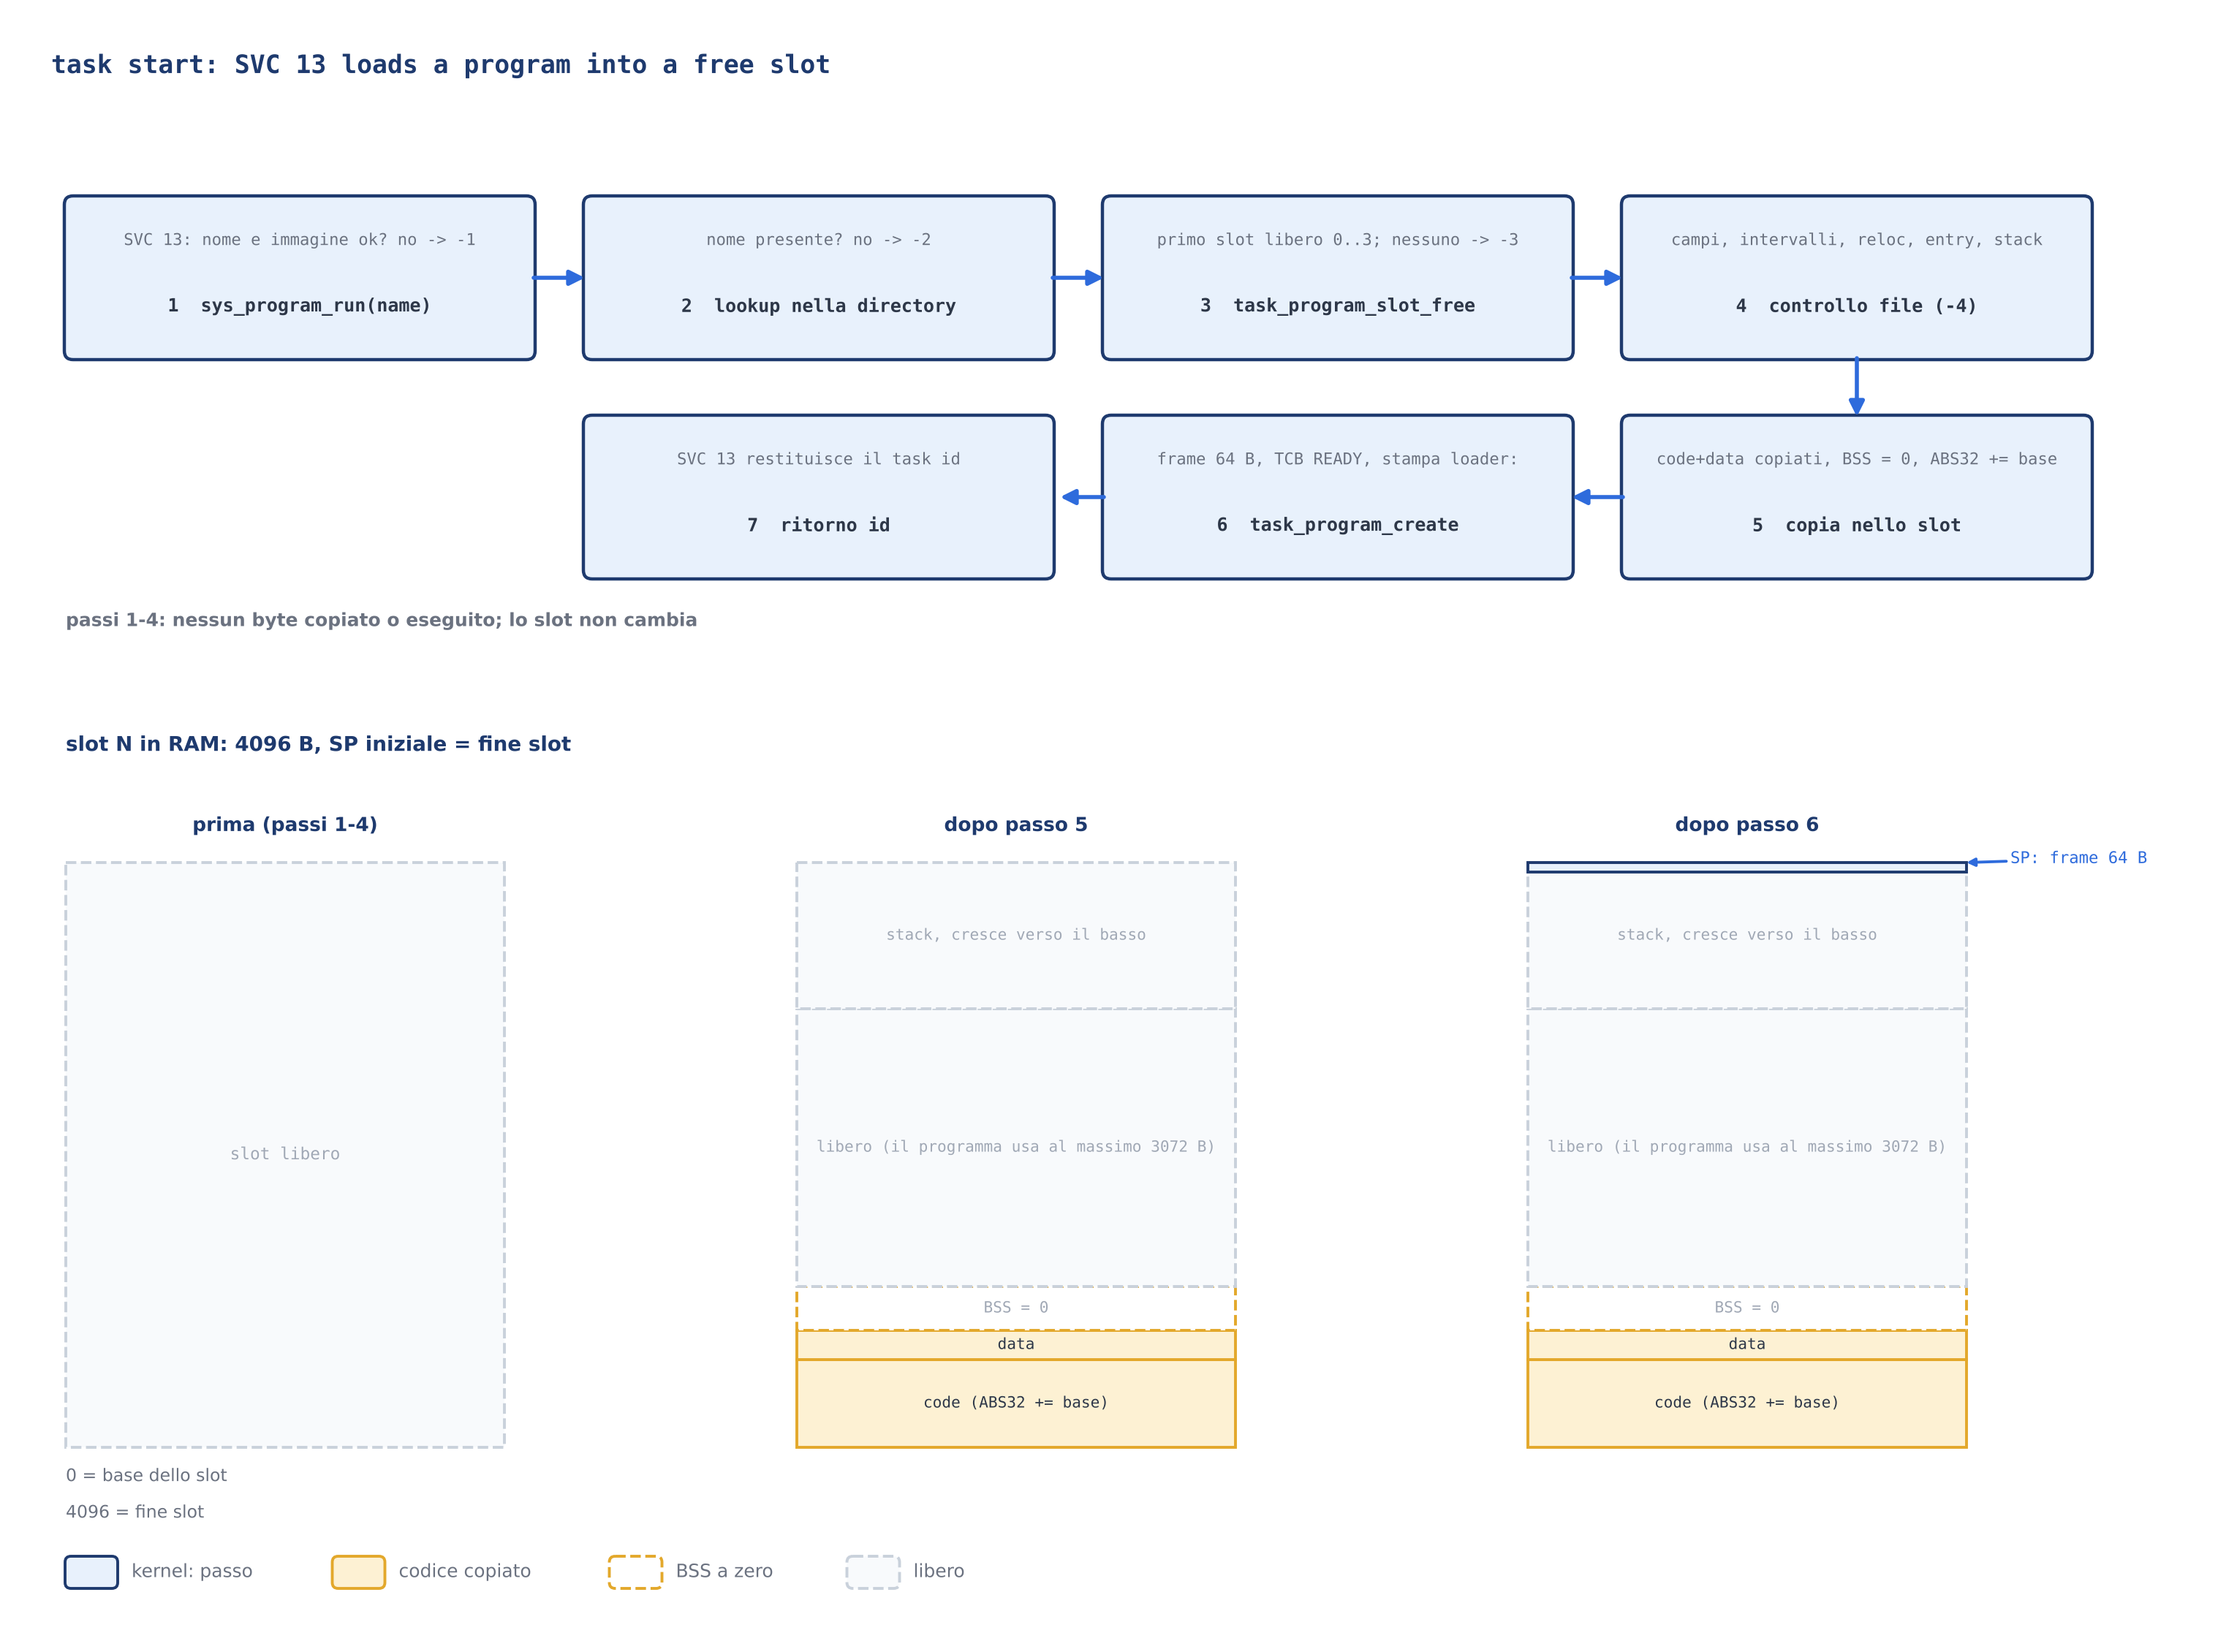
\includegraphics[width=1\textwidth]{contents/images/project/prj_task_start.png}
    \caption{Caricamento di un programma con SVC 13: i passi 1--4 controllano tutto senza scrivere nello slot, dal passo 5 la copia riempie lo slot e il passo 6 crea il task. In basso, lo stato dello slot dopo il passo 5 e dopo il passo 6.}
    
\end{figure}

\subsection{Esecuzione}
\begin{enumerate}\sloppy\setcounter{enumi}{15}
\item La shell chiama la SVC 14 con l'id ricevuto e passa nello stato WAITING. Il programma può anche partire prima che la shell chiami la SVC 14.
\item Il programma gira unprivileged in Thread mode, sul PSP, con codice e dati nel suo slot; la MPU, programmata a ogni task switch, lo confina nello slot. \texttt{\_start} chiama \texttt{main}.
\end{enumerate}

\subsection{Fine del programma}
\begin{enumerate}\sloppy\setcounter{enumi}{17}
\item Ritorno da \texttt{main} o \texttt{sys\_exit()}: il sistema stampa \texttt{program <name> exited} e lo stato di fine è 0.
\item Fault recuperabile: il sistema stampa la riga del fault e \texttt{program <name> faulted}; lo stato di fine è \texttt{-2}.
\item In entrambi i casi il codice dato salva lo stato, mette direttamente il task record in UNUSED, sveglia i task in attesa e chiede un task switch: lo slot è subito riusabile.
\item La SVC 14 della shell restituisce lo stato, che la shell ignora perché il kernel ha già stampato come è finito il programma, e la shell stampa di nuovo il prompt.
\item Fault non recuperabile: il sistema stampa la riga \texttt{unrecoverable} e si ferma, senza prompt.
\end{enumerate}

\begin{figure}[H]
    \centering
    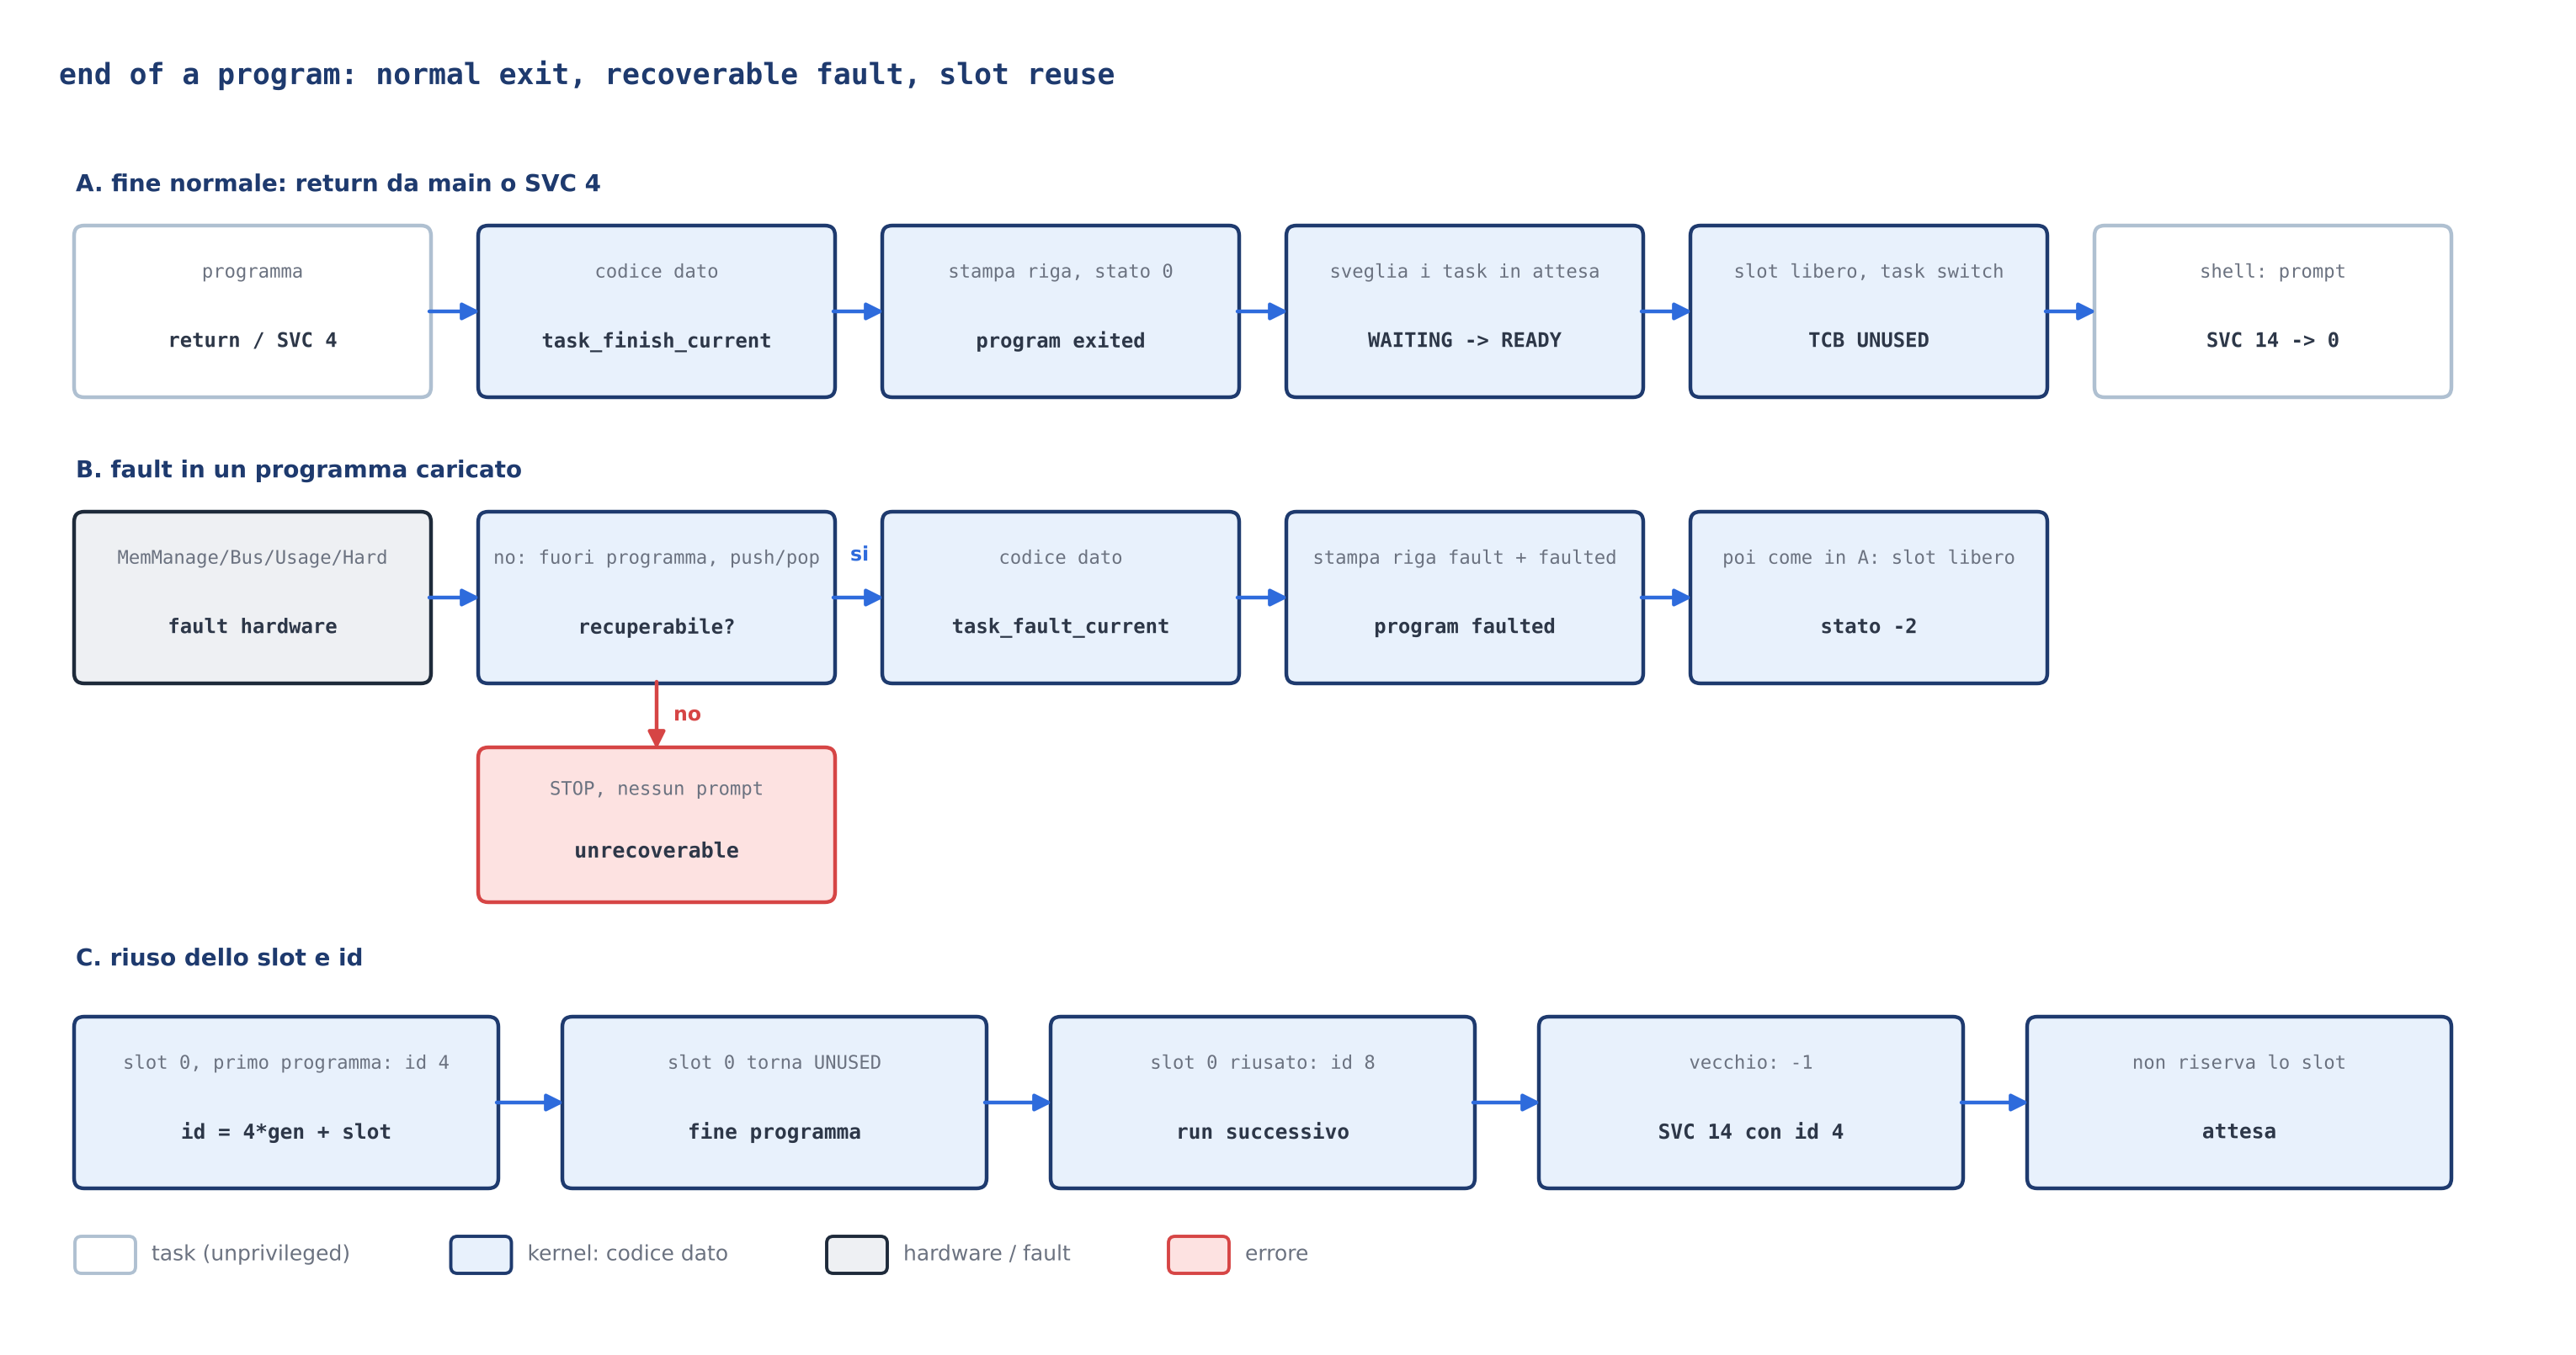
\includegraphics[width=1\textwidth]{contents/images/project/prj_task_end.png}
    \caption{Fine di un programma: uscita normale, fault recuperabile e riuso dello slot. Il codice dato libera lo slot subito e riporta il prompt; un fault non recuperabile ferma invece il sistema.}
    
\end{figure}

\begin{figure}[H]
    \centering
    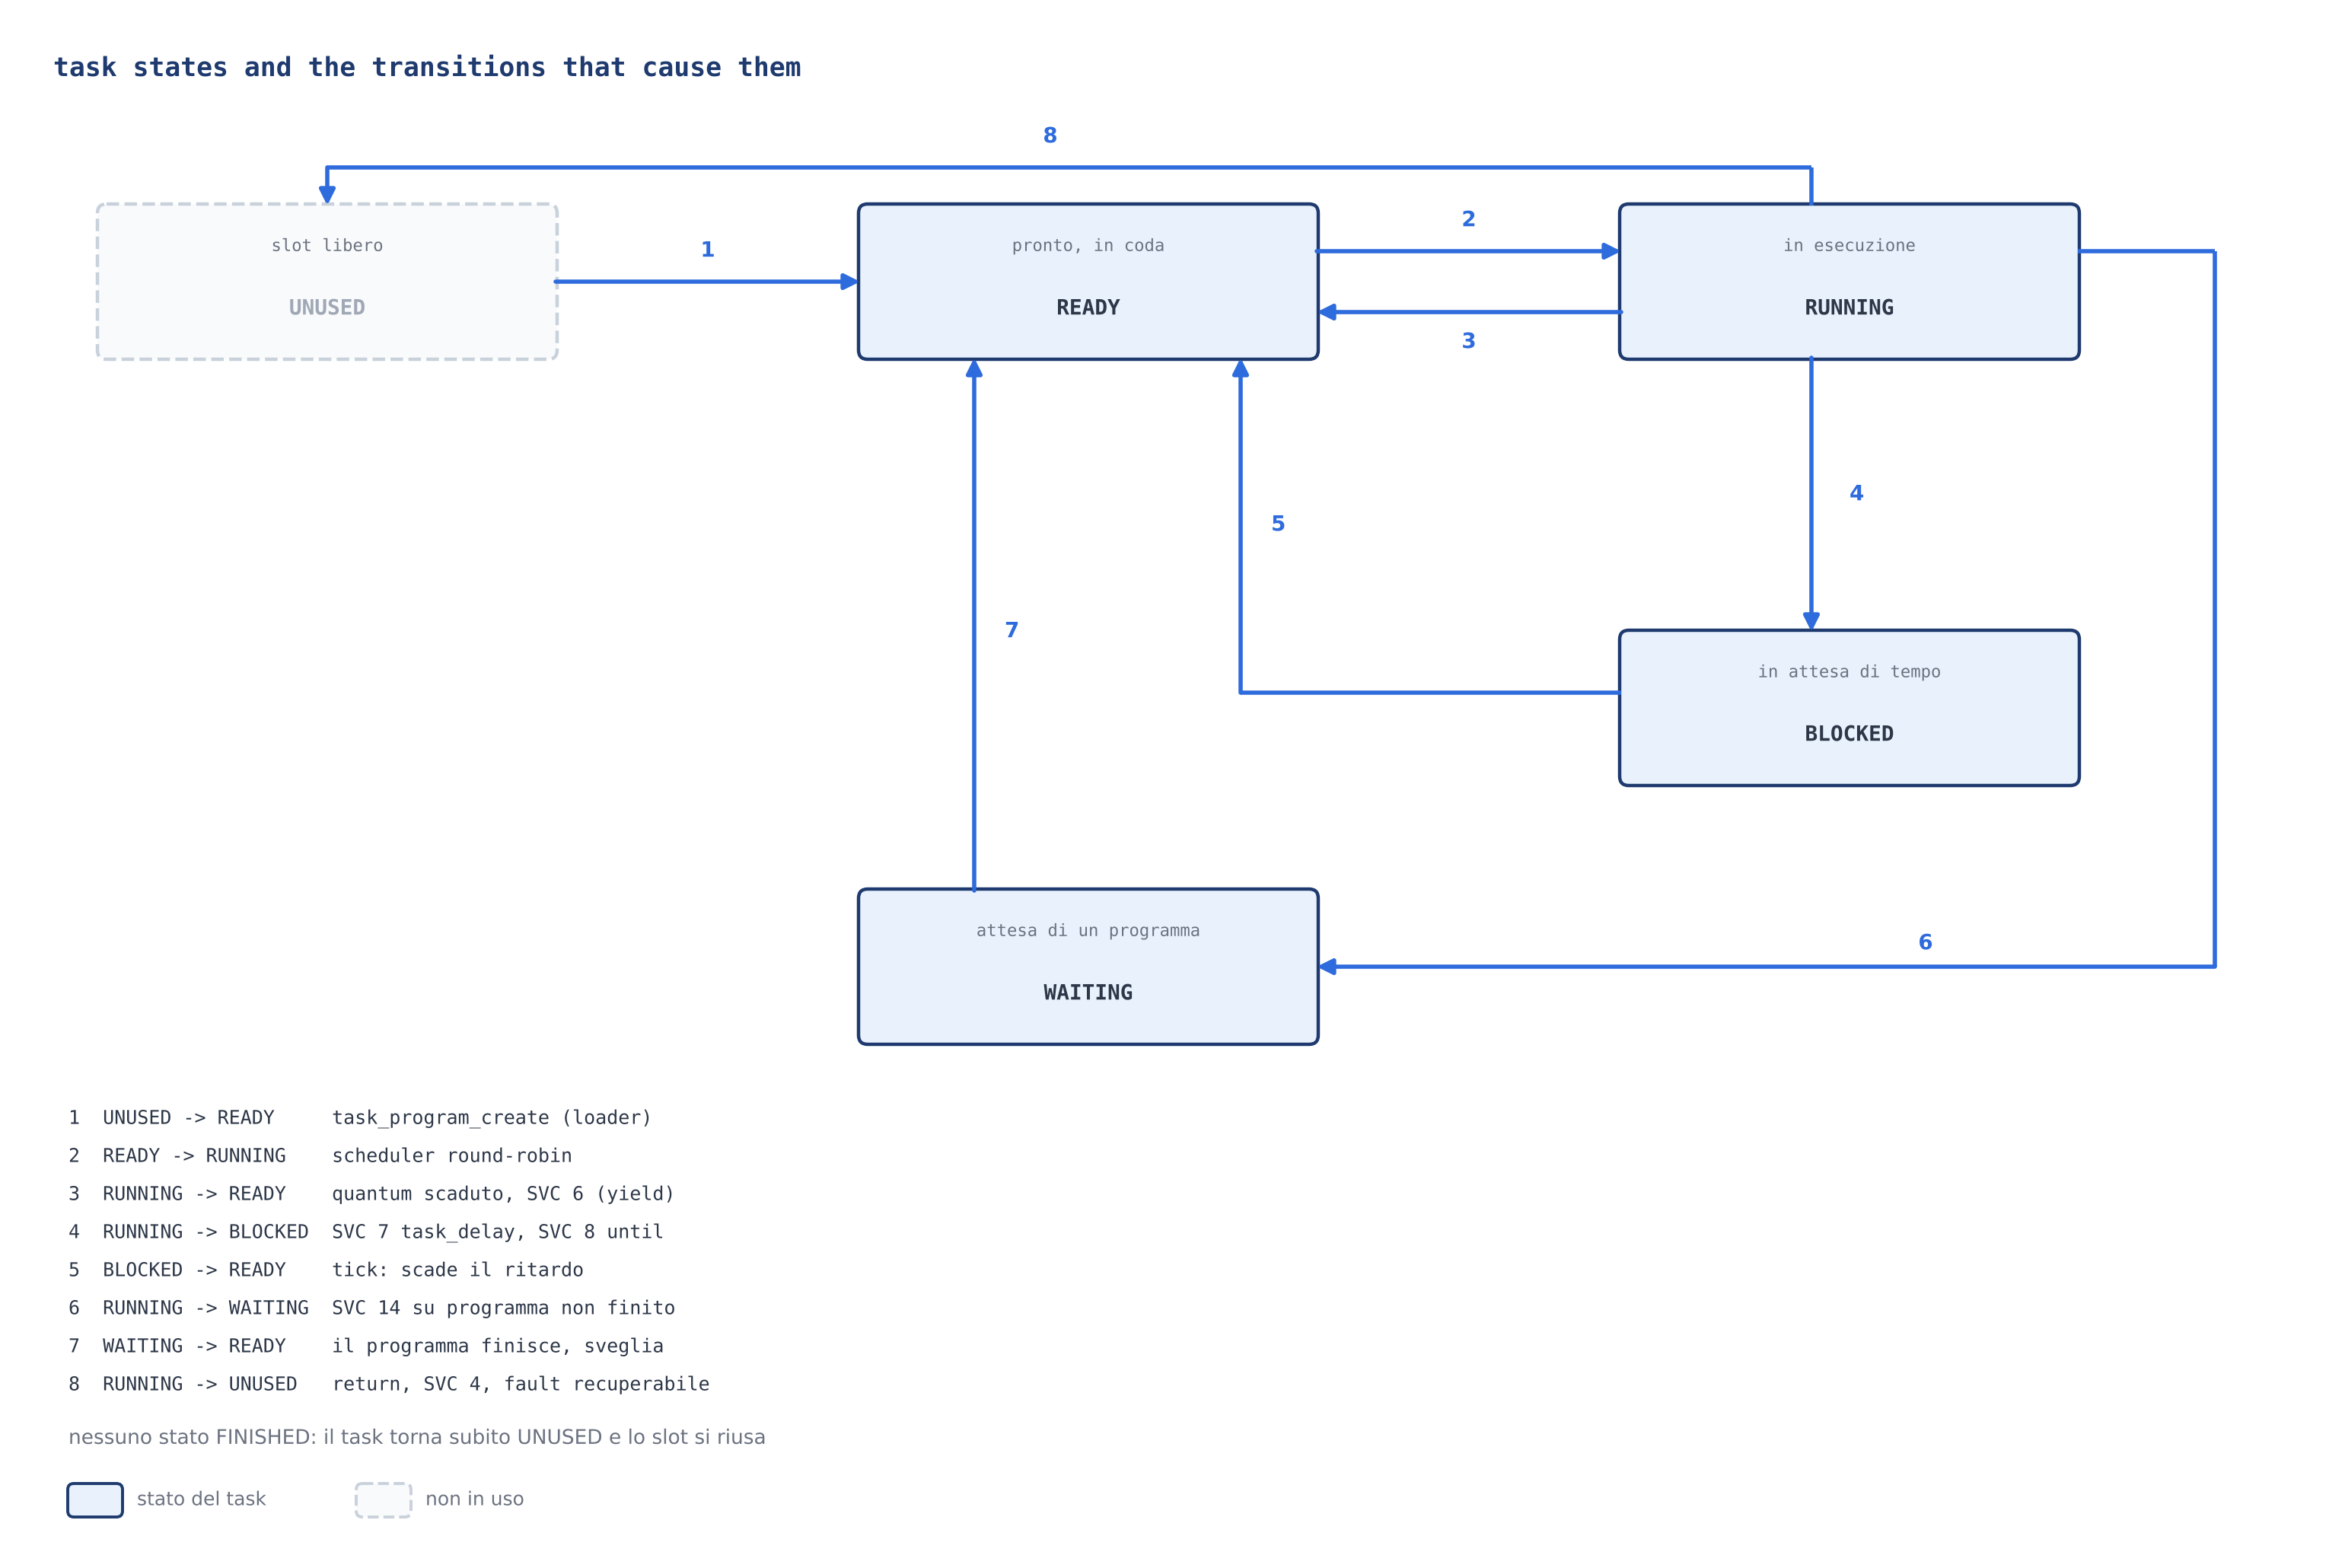
\includegraphics[width=1\textwidth]{contents/images/project/prj_states.png}
    \caption{Stati dei task e transizioni, con la funzione o la SVC che le causa. Il progetto non introduce uno stato FINISHED: un programma terminato rende lo slot subito \texttt{UNUSED}.}
    
\end{figure}

\section{Vincoli e divieti}

\subsection{Che cosa non si può fare}
\begin{itemize}\sloppy
\item Sostituire o copiare il codice dato del ciclo di vita dei programmi e del recupero dai fault: deve restare lui al comando.
\item Aggiungere un altro modo di aspettare un programma attraverso l'helper del kernel di \texttt{task\_wait\_program}.
\item Scrivere nell'immagine o copiarla intera in RAM.
\item Copiare o eseguire un qualunque byte del programma prima di aver finito tutti i controlli. Un caricamento fallito e il tentativo di avviare un quinto programma mentre ne girano quattro non devono cambiare nessuno slot.
\item Chiamare \texttt{task\_program\_create} prima che il programma sia caricato per intero e senza errori.
\item Stampare comandi extra o output di debug: non devono mai comparire nelle trascrizioni, né ritardarle o cambiarle.
\item Far condividere codice tra programmi e kernel, o usare nei programmi la libreria C o un heap.
\item Produrre ELF con record \texttt{RELA}, dynamic linking, simboli non definiti o altri tipi di relocation per il contenuto caricato.
\item Rendere recuperabili i fault durante il salvataggio dello stack frame, i fault nel kernel e quelli fuori dai programmi caricati: devono restare non recuperabili.
\item Cambiare, con programmi o test extra della squadra, i comandi, l'output, i formati o il comportamento dei test fissati.
\item Nella big, lasciare una regione MPU sovrapposta con lettura, scrittura ed esecuzione: romperebbe W\textasciicircum{}X.
\end{itemize}

\subsection{Che cosa si può cambiare}
\begin{itemize}\sloppy
\item Si possono aggiungere moduli e aggiungere campi al codice delle system call, dei task e della MPU.
\item Le squadre big possono aggiungere campi ai task record ed estendere il setup MPU di ogni task switch, purché il comportamento dato resti lo stesso.
\item La ricetta \texttt{make image} della base va cambiata ().
\end{itemize}

\subsection{Che cosa è fisso e che cosa decide la squadra}

\begin{center}
\small
\begin{tabular}{|p{0.44\linewidth}|p{0.44\linewidth}|}
\hline
\raggedright Fisso per tutte le squadre & \raggedright Deciso dalla squadra \tabularnewline
\hline\hline
\raggedright Board e CPU di QEMU, indirizzo dell'immagine e limite di dimensione, formato IMG1 e suoi limiti & \raggedright Organizzazione di moduli e file \tabularnewline
\hline
\raggedright Versione assegnata in base alla dimensione della squadra & \raggedright Organizzazione e coordinamento del lavoro tra i membri \tabularnewline
\hline
\raggedright Indirizzi, dimensione e allineamento degli slot, scelta del primo libero, limite di 3072 byte per il programma, stack di 1024 byte & \raggedright Funzioni di supporto per i controlli e strutture dati interne, purché calcoli e intervalli siano sicuri \tabularnewline
\hline
\raggedright Numeri, argomenti e risultati delle system call, regole sui puntatori, task id, ciclo di vita dei programmi & \raggedright Nomi delle funzioni del kernel, tranne i punti di integrazione dati \tabularnewline
\hline
\raggedright Comandi, prompt, output, limite dell'input e messaggi d'errore della shell & \raggedright Struttura della shell e modo in cui bufferizza l'input \tabularnewline
\hline
\raggedright Regole di build dei programmi: link all'indirizzo zero, entry Thumb, \texttt{--emit-relocs}, ritorno da \texttt{main} che vale come exit & \raggedright Programmi di prova privati in più e test lato host \tabularnewline
\hline
\raggedright Small: formato SFT1, regole di conversione e di relocation, una regione MPU con lettura, scrittura ed esecuzione & \raggedright Struttura del lettore ELF lato host (non serve nessuna libreria esterna) \tabularnewline
\hline
\raggedright Big: ELF salvato invariato, sottoinsieme ELF richiesto, relocation e controlli, messaggio con il tipo numerico & \raggedright Struttura del lettore ELF nel kernel; il contenuto non usato non va controllato \tabularnewline
\hline
\raggedright Big: codice lettura + esecuzione; dati e stack lettura + scrittura, non eseguibili & \raggedright Quali regioni MPU danno questi permessi \tabularnewline
\hline
\raggedright Codice e chiamate dati del ciclo di vita & \raggedright Stile della documentazione e della presentazione \tabularnewline
\hline
\raggedright Test suite e trascrizioni, punti, penalità & \raggedright Funzioni extra che non cambiano nessun comportamento fisso \tabularnewline
\hline
\end{tabular}
\end{center}

\subsection{Regole di stile e di codice}

Il .md non impone uno stile di scrittura del codice. Le regole pratiche vengono dal criterio di efficienza e dai controlli richiesti:
\begin{itemize}
\item uso delle risorse limitato (bounded);
\item nessuna copia inutile dell'immagine e nessuna allocazione dinamica;
\item controlli chiari e ben strutturati, senza duplicazioni evitabili;
\item ogni calcolo su offset, dimensioni e intervalli protetto dall'overflow;
\item per leggere gli ELF lato host non serve nessuna libreria esterna.
\end{itemize}

\section{Comandi}

Il .md riporta solo i comandi seguenti. Il comando completo di build (per esempio il target del Makefile che crea programmi e immagine) lo sceglie la squadra e va scritto nella documentazione.

\subsection{Build ed esecuzione}

\texttt{make run} compila la base e la avvia in QEMU, usando un'immagine già esistente; \texttt{make image} è la ricetta della base per l'immagine, da cambiare.
\begin{lstlisting}[language=bash]
# Compila e avvia in QEMU; usa un'immagine esistente
make run
# Ricetta della base per l'immagine: da cambiare
make image
\end{lstlisting}

Questa è l'opzione con cui QEMU carica l'immagine nella FLASH, senza modificarla, a partire dall'indirizzo \texttt{0x00200000}:
\begin{lstlisting}[language=bash]
-device loader,file=build/fs.img,addr=0x00200000,force-raw=on
\end{lstlisting}

\subsection{Host tool}

\texttt{flat} (solo small) converte un ELF in SFT1; \texttt{image} crea \texttt{build/fs.img} dai programmi elencati, nell'ordine dato.
\begin{lstlisting}[language=bash]
# Small: converte un ELF in un file SFT1
python3 tools/mkimage.py flat PROGRAM.elf PROGRAM.sft
# Small e big: crea build/fs.img (IMG1)
python3 tools/mkimage.py image build/fs.img NAME=PROGRAM.elf [NAME=PROGRAM.elf ...]
\end{lstlisting}

\subsection{Test}

Il runner esegue la suite small (10 test) o big (14 test).
\begin{lstlisting}[language=bash]
# Suite small
python3 run_tests.py --suite small --kernel KERNEL.axf --image fs.img
# Suite big
python3 run_tests.py --suite big --kernel KERNEL.axf --image fs.img
\end{lstlisting}
\texttt{KERNEL.axf} e \texttt{fs.img} stanno al posto dei percorsi veri: il runner usa come kernel \texttt{build/scratch-os.axf}, e l'immagine della squadra è \texttt{build/fs.img}. Il runner si lancia dalla cartella del test kit, oppure da un'altra cartella con i percorsi giusti di kernel e immagine.

\begin{center}
\small
\begin{tabular}{|l|p{0.55\linewidth}|}
\hline
Opzione & \raggedright Effetto \tabularnewline
\hline\hline
\texttt{--list} & \raggedright elenca i test \tabularnewline
\hline
\texttt{--test NAME} & \raggedright esegue solo il test indicato; si può ripetere \tabularnewline
\hline
\texttt{--startup-timeout} & \raggedright limite di tempo per l'avvio (default 5 secondi) \tabularnewline
\hline
\texttt{--test-timeout} & \raggedright limite di tempo per ogni test (default 5 secondi) \tabularnewline
\hline
\texttt{--global-timeout} & \raggedright limite di tempo per l'intera esecuzione (default 90 secondi) \tabularnewline
\hline
\end{tabular}
\end{center}

Stato di uscita del runner: 0 se la suite passa, 1 per test falliti o problemi di QEMU, 2 per errori di configurazione.

\subsection{Ispezione e debug}

Per vedere header, entry point, sezioni caricate e relocation di un programma si usano gli strumenti ARM bare-metal \texttt{readelf} (\texttt{arm-none-eabi-readelf}), \texttt{objdump}, \texttt{nm} e \texttt{size}. Il file \texttt{build/output.map} mostra i simboli del linker del kernel.

GDB non sa in quale slot è stato caricato un programma, quindi bisogna dirglielo con il comando seguente.
\begin{lstlisting}[language=bash]
# In GDB: simboli di un programma all'indirizzo del suo slot
add-symbol-file PROGRAM.elf LOAD_ADDRESS
# Esempio: thumb_ptr caricato nello slot 1
add-symbol-file build/programs/thumb_ptr.elf 0x20003000
\end{lstlisting}
Si usa l'indirizzo dello slot in RAM, non quello del file dentro l'immagine. \emph{Da chiarire con il professore:} il .md non dice come avviare QEMU e GDB per una sessione di debug.

\section{Piano di lavoro consigliato}

Il .md dice esplicitamente che i requisiti non sono un piano di lavoro e che ordine e divisione del lavoro li decide la squadra. Quella che segue è quindi una \emph{proposta}: ogni passo si appoggia sui precedenti e finisce con un traguardo verificabile.

\begin{enumerate}\sloppy
\item \emph{Partire dalla base.} Compilare e avviare \texttt{scratch-os/project-base/} con \texttt{make run}; leggere \texttt{kernel/task.h}, il linker script della base e \texttt{build/output.map}.\newline
Traguardo: la base parte in QEMU, ancora senza shell né loader.
\item \emph{Shell (R4).} Definire \texttt{task\_project\_configure()} e configurare la shell con \texttt{task\_configure\_shell()}; prompt, eco, limite di 31 caratteri, \texttt{help} ed \texttt{error:\ unknown command}.\newline
Traguardo: righe di boot, prompt e output di \texttt{help} identici a quelli di .
\item \emph{Build dei programmi (R1).} Startup texttt, linker script all'indirizzo \texttt{0}, \texttt{--emit-relocs}, stub e \texttt{printf} propri.\newline
Traguardo: \texttt{arm-none-eabi-readelf} mostra un \texttt{ET\_EXEC} con entry Thumb, almeno un \texttt{PT\_LOAD} e le sezioni \texttt{REL}.
\item \emph{Host tool (R2).} Comando \texttt{image} (più \texttt{flat} nella small) e ricetta \texttt{make image} aggiornata.\newline
Traguardo: messaggi di successo esatti; input sbagliati rifiutati con stato 2 prima di scrivere output.
\item \emph{Lettura dell'immagine (R3) e SVC 11 e 12 (R5).}\newline
Traguardo: \texttt{ls} elenca i programmi; con un'immagine non valida stampa \texttt{error:\ no valid image}.
\item \emph{Loader (R6, R5, R9; nella big anche B1).} SVC 13 con tutti i controlli, copia, BSS, relocation e \texttt{task\_program\_create}; SVC 14 nella shell. Small: file SFT1; big: ELF letti dal kernel.\newline
Traguardo: \texttt{run} produce la sessione di ; passano \texttt{global\_state}, \texttt{thumb\_ptr} e \texttt{nonzero\_slot\_relocation}.
\item \emph{MPU e fine dei programmi (R7, R8; nella big anche B2).}\newline
Traguardo: passano \texttt{normal\_return}, \texttt{explicit\_exit} e \texttt{kernel\_store}; nella big anche \texttt{wx\_write\_texttt} e \texttt{wx\_exec\_data}.
\item \emph{Robustezza (R9).} Immagini e file malformati, argomenti sbagliati delle system call.\newline
Traguardo: passano \texttt{bad\_magic}, \texttt{bad\_header}, \texttt{too\_large} e \texttt{bad\_reloc}; nella big anche \texttt{unsupported\_reloc} e \texttt{truncated\_elf}.
\item \emph{Suite completa.}\newline
Traguardo: la riga \texttt{SUMMARY} riporta \texttt{failed=0}, cioè 10 test su 10 (small) o 14 su 14 (big), con \texttt{build/scratch-os.axf} e \texttt{build/fs.img} ricostruiti da zero.
\item \emph{Documentazione e demo.}\newline
Traguardo: la documentazione contiene tutte le voci di  e la demo mostra i cinque punti richiesti.
\end{enumerate}

\begin{figure}[H]
    \centering
    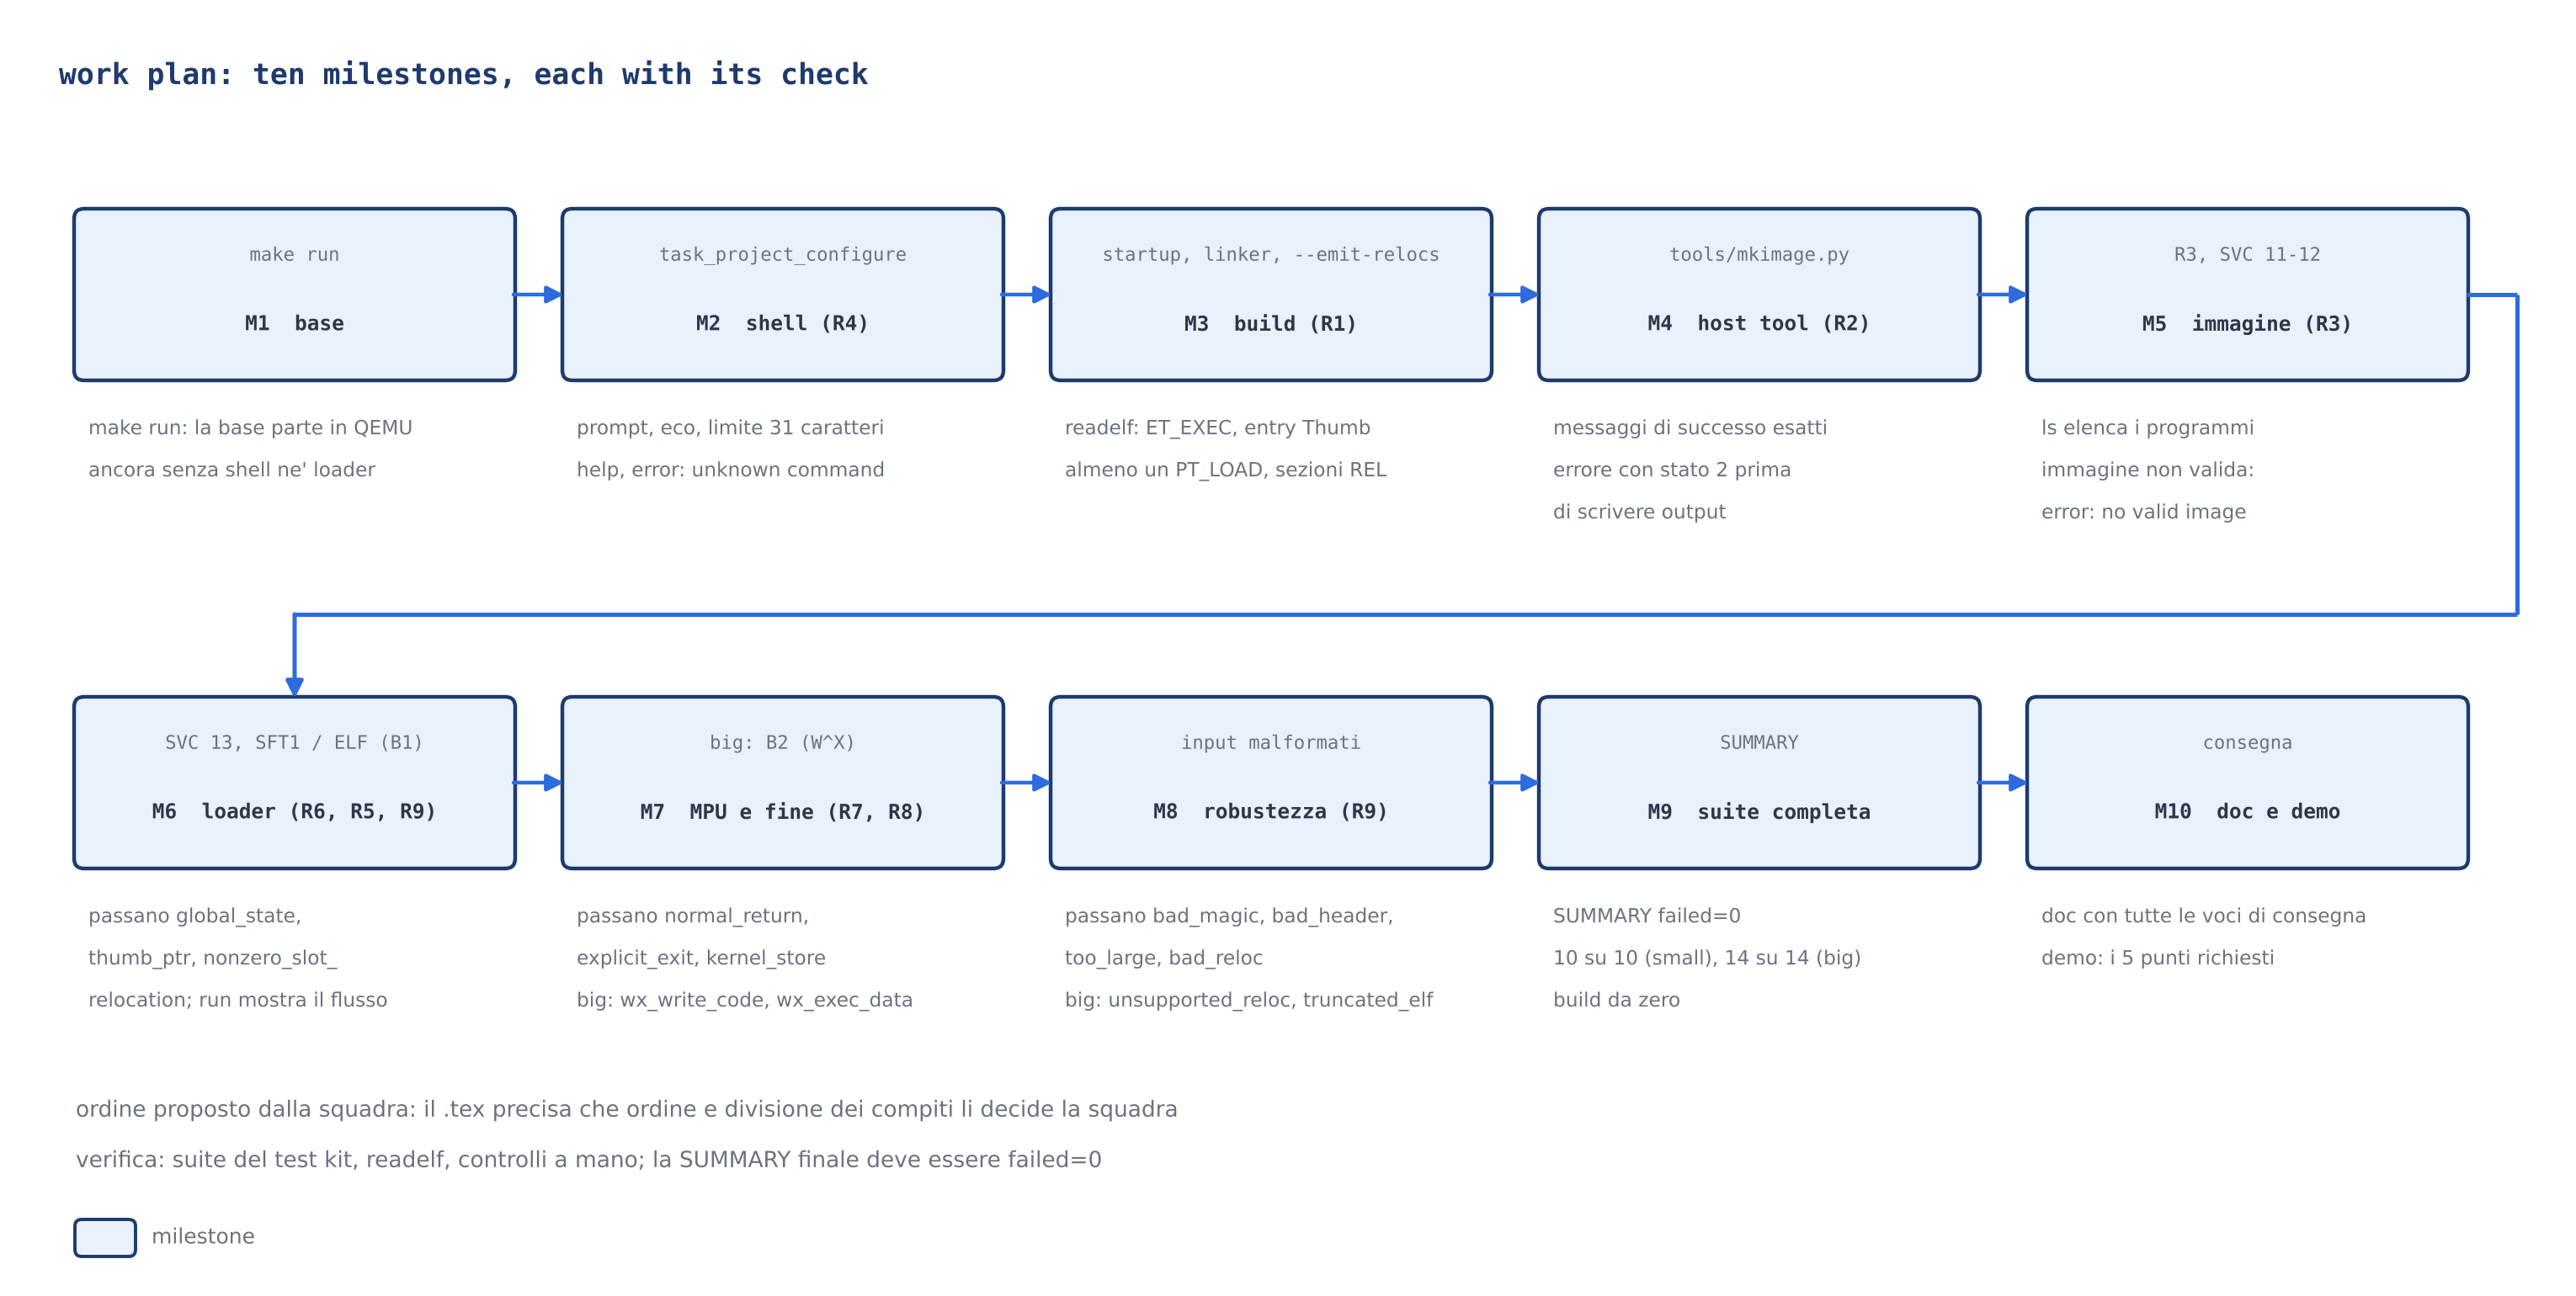
\includegraphics[width=1\textwidth]{contents/images/project/prj_roadmap.png}
    \caption{Piano di lavoro proposto: dieci milestone in sequenza, ciascuna con il criterio con cui verificare che funzioni. La squadra può cambiare l'ordine, ma ogni milestone deve chiudersi con la verifica indicata.}
\end{figure}

\section{Test e verifica}

\subsection{Come controlla il professore}
\begin{itemize}\sloppy
\item Usa lo stesso test kit pubblicato, con la suite della versione della squadra, sullo stato del repository alla scadenza. Come kernel il runner usa \texttt{build/scratch-os.axf}.
\item Ogni test avvia un QEMU nuovo e confronta tutto ciò che viene stampato sulla UART con l'output atteso. Solo i fine riga CRLF dell'host diventano LF; ogni altro byte deve coincidere.
\item Le trascrizioni attese contengono anche le due righe di boot, i comandi con la loro eco, le righe del loader e di fine, e ogni prompt \texttt{scratch> }: deve coincidere l'intera trascrizione.
\item I test valgono al massimo 1.50 punti, in proporzione ai test superati (). Il resto del voto viene dalla valutazione dei requisiti, dalla presentazione con demo e dalle domande individuali.
\end{itemize}

\subsection{Il test kit}

Il test kit è nella cartella \texttt{test-kit/} accanto al documento della consegna (in \texttt{Projects.md} il link è \texttt{project/test-kit/}). Contiene \texttt{run\_tests.py}, i sorgenti dei programmi di test, i generatori riproducibili dei file rotti (le fixture), le definizioni delle suite (i manifest) e le trascrizioni attese.

Per ogni test il runner stampa una di queste due righe, e QEMU si ferma dopo ogni risultato:
\begin{itemize}\sloppy
\item \texttt{PASS <name>} se il test passa;
\item \texttt{FAIL <name>:\ <reason>} se fallisce.
\end{itemize}
L'esecuzione finisce con:
\begin{lstlisting}
SUMMARY suite=<suite> passed=<passed> failed=<failed> total=<total>
\end{lstlisting}

\emph{Da chiarire con il professore:} il test kit non è allegato e il .md non spiega che cosa deve contenere l'immagine passata con \texttt{--image} (quali programmi di test e con quali nomi), né come i file rotti prodotti dai generatori finiscono nell'immagine.

\subsection{I test}

La suite small ha 10 test. La suite big esegue gli stessi dieci test con file ELF e ne aggiunge quattro solo big, per un totale di 14.

I dieci test comuni:

\begin{center}
\small
\begin{tabular}{|p{0.33\linewidth}|p{0.57\linewidth}|}
\hline
\raggedright Test & \raggedright Che cosa controlla \tabularnewline
\hline\hline
\raggedright \texttt{nonzero\_\allowbreak slot\_\allowbreak relocation} & \raggedright Un programma padre gira nello slot 0 (base \texttt{0x20002000}, id 4); il figlio gira nello slot 1 (base \texttt{0x20003000}, id 5) e stampa \texttt{thumb\_function\_pointer:\ thumb=1 result=42}. Il padre riceve 0. \tabularnewline
\hline
\raggedright \texttt{global\_state} & \raggedright Slot 0, id 4: stampa \texttt{globals\_bss\_const:\ global=37 bss=0 table=16 sum=53}, poi esce. \tabularnewline
\hline
\raggedright \texttt{thumb\_ptr} & \raggedright Slot 0, id 4: stampa \texttt{thumb\_function\_pointer:\ thumb=1 result=42}, poi esce. \tabularnewline
\hline
\raggedright \texttt{normal\_return} & \raggedright Torna da \texttt{main}: \texttt{normal\_return:\ returning from main}, poi \texttt{program normal\_return exited}. \tabularnewline
\hline
\raggedright \texttt{explicit\_exit} & \raggedright Chiama la SVC 4: \texttt{explicit\_exit:\ calling sys\_exit}, poi \texttt{program explicit\_exit exited}. \tabularnewline
\hline
\raggedright \texttt{kernel\_store} & \raggedright Scrive a \texttt{0x20000000}: \texttt{MemManage in loaded program:\ CFSR=0x82 address=0x20000000}. Poi \texttt{print\_plain} riusa lo slot 0 con id 8. \tabularnewline
\hline
\raggedright \texttt{bad\_magic} & \raggedright Rifiutato; poi \texttt{help} mostra che la shell funziona ancora. \tabularnewline
\hline
\raggedright \texttt{bad\_header} & \raggedright Rifiutato; poi \texttt{help} mostra che la shell funziona ancora. \tabularnewline
\hline
\raggedright \texttt{too\_large} & \raggedright Un programma da 3076 byte viene rifiutato; poi \texttt{help} mostra che la shell funziona ancora. \tabularnewline
\hline
\raggedright \texttt{bad\_reloc} & \raggedright Una relocation fuori dal programma viene rifiutata; poi \texttt{help} mostra che la shell funziona ancora. \tabularnewline
\hline
\end{tabular}
\end{center}

I quattro test solo big:

\begin{center}
\small
\begin{tabular}{|p{0.33\linewidth}|p{0.57\linewidth}|}
\hline
\raggedright Test & \raggedright Che cosa controlla \tabularnewline
\hline\hline
\raggedright \texttt{unsupported\_reloc} & \raggedright Il tipo 3 stampa \texttt{loader:\ unsupported relocation type 3}. Poi un programma corretto gira nello slot 0 con id 4. \tabularnewline
\hline
\raggedright \texttt{truncated\_elf} & \raggedright Un ELF tagliato viene rifiutato senza nessuna riga di fault. Poi un programma corretto gira nello slot 0 con id 4. \tabularnewline
\hline
\raggedright \texttt{wx\_write\_texttt} & \raggedright Una scrittura nel codice stampa \texttt{MemManage in loaded program:\ CFSR=0x82 address=0x20002280}. Poi un programma corretto riusa lo slot 0 con id 8. \tabularnewline
\hline
\raggedright \texttt{wx\_exec\_data} & \raggedright Un salto nei dati stampa \texttt{MemManage in loaded program:\ CFSR=0x1}. Poi un programma corretto riusa lo slot 0 con id 8. \tabularnewline
\hline
\end{tabular}
\end{center}

\subsection{Come verificare da soli prima di consegnare}
\begin{itemize}\sloppy
\item Ricostruire tutto da zero (programmi, \texttt{build/fs.img}, \texttt{build/scratch-os.axf}) con i comandi scritti nella documentazione.
\item Eseguire la suite della propria versione e ottenere \texttt{failed=0}; per isolare un test che fallisce, usare \texttt{--list} e \texttt{--test NAME}.
\item Ripetere i test sullo stato effettivamente presente nel repository GitLab, perché la valutazione usa quello alla scadenza.
\item Ispezionare i programmi con \texttt{arm-none-eabi-readelf}: header, entry point, sezioni caricate e relocation.
\item Controllare i permessi MPU che risultano dopo ogni task switch.
\item Verificare che sulla UART non esca nessuna riga di debug.
\item Provare la demo completa: caricamento normale, relocation in uno slot diverso da 0, rifiuto di un input sbagliato, recupero da un fault e comportamento specifico della versione.
\end{itemize}

\section{Consegna}

\paragraph{Dove.} Ogni squadra riceve account GitLab del corso: il lavoro si tiene e si consegna in quel repository.

\paragraph{Quando.} Non c'è una data di inizio obbligatoria. Il progetto va completato entro la fine dell'anno accademico, e la valutazione usa lo stato del repository alla scadenza. Le squadre si formano entro il 16 ottobre (). \emph{Da chiarire con il professore:} la data esatta della scadenza di consegna e quando si tiene la presentazione.

\paragraph{Che cosa consegnare.}
\begin{itemize}\sloppy
\item Tutti i sorgenti e i file di build che servono per ricompilare il kernel e tutti i programmi.
\item \texttt{tools/mkimage.py} e \texttt{build/fs.img}.
\item Il kernel eseguibile \texttt{build/scratch-os.axf}, che il test runner usa come kernel.
\item Nessun file oggetto generato, tranne l'immagine richiesta e il kernel eseguibile.
\end{itemize}

\paragraph{Documentazione.} Deve contenere:
\begin{itemize}
\item i prerequisiti;
\item i comandi esatti di build, esecuzione e test;
\item le scelte di progetto e di formato;
\item come la squadra ha integrato la MPU e il codice dato del ciclo di vita;
\item i limiti noti;
\item la procedura esatta della demo.
\end{itemize}
Nel complesso deve dare informazioni sufficienti per riprodurre il risultato consegnato.

\paragraph{Presentazione e demo.} È una presentazione orale di 20 minuti con tutti i membri, seguita da domande individuali e da una demo dal vivo. La demo deve mostrare: caricamento normale, relocation in uno slot diverso da 0, rifiuto di un input sbagliato, recupero da un fault e il comportamento specifico della versione.

\paragraph{Regole per i membri.} Ogni membro deve capire tutto il progetto, anche il codice scritto dagli altri: il professore può chiedere a chiunque qualunque parte, e ogni risposta conta per il voto di quello studente.

\begin{figure}[H]
    \centering
    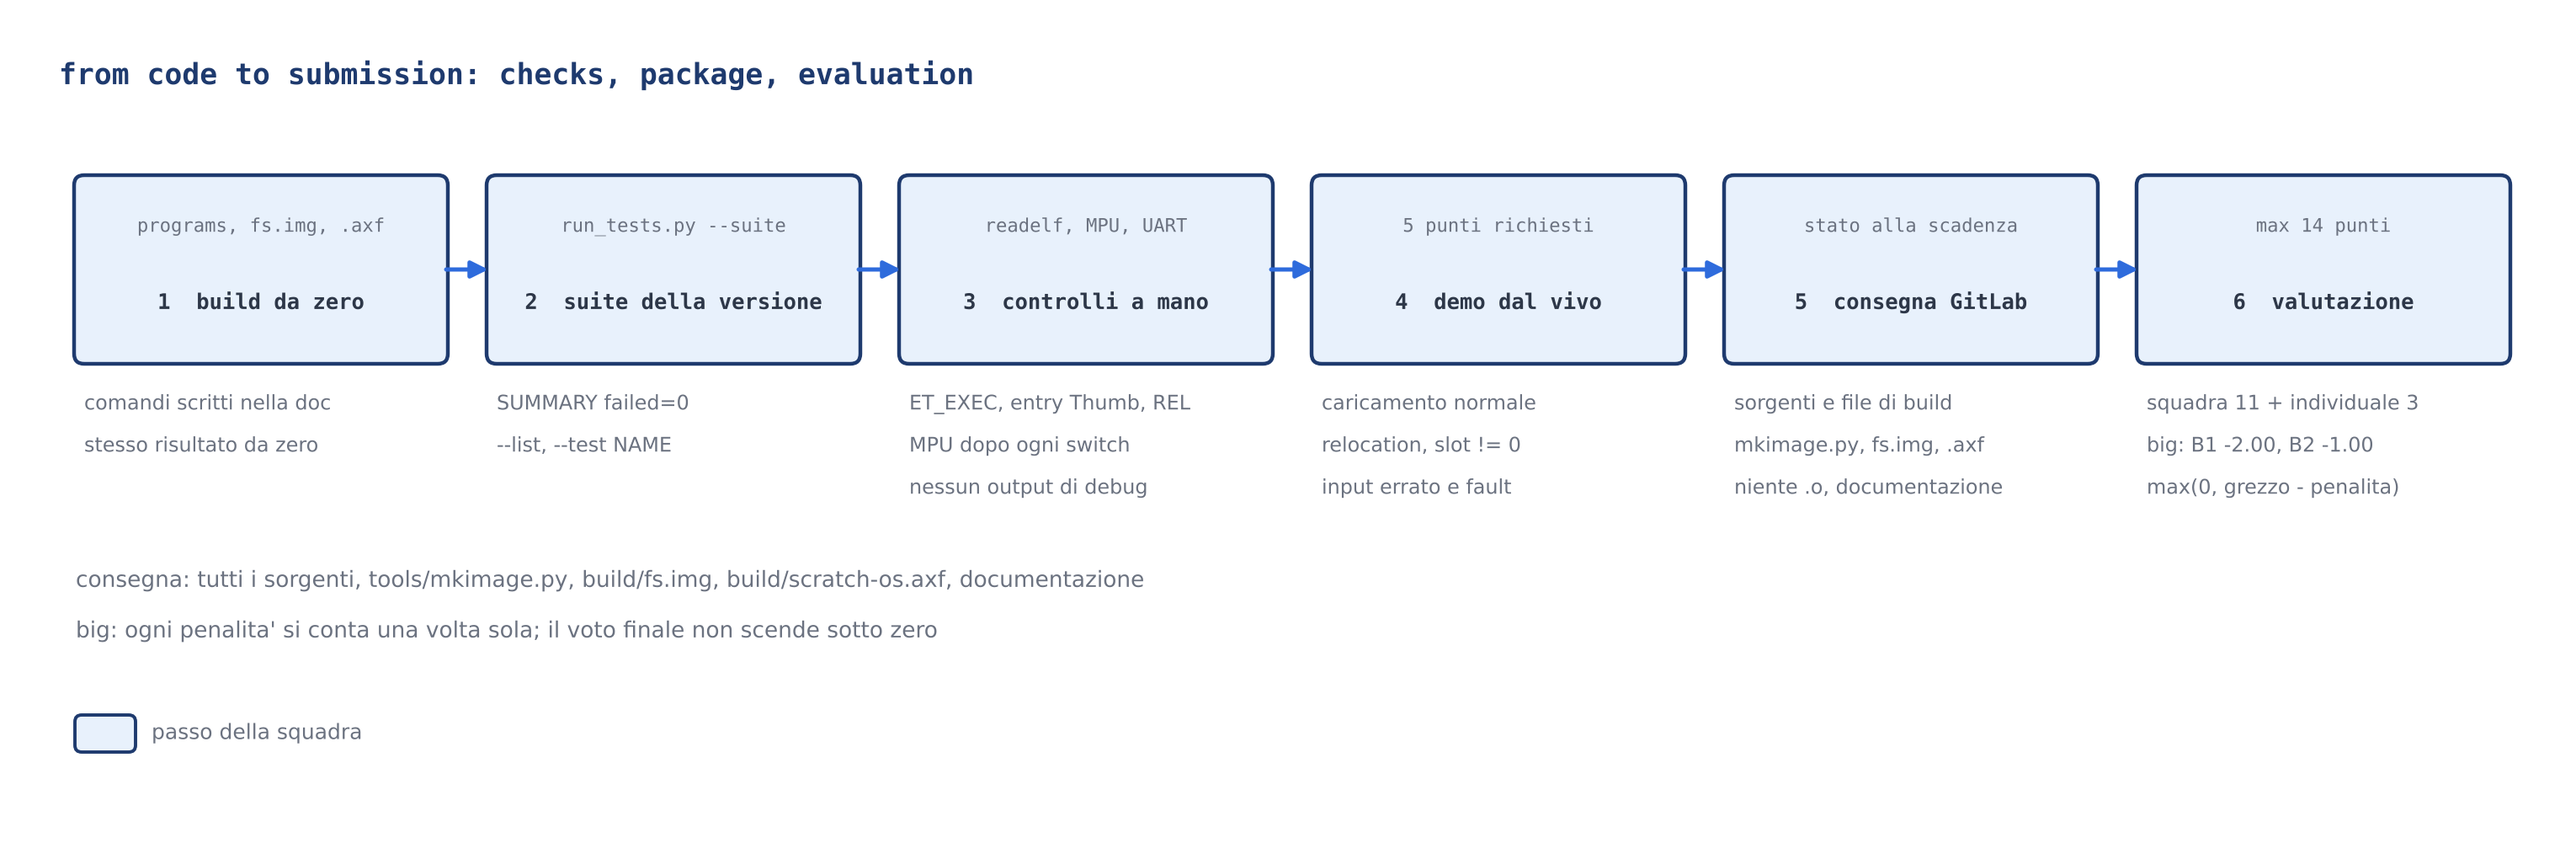
\includegraphics[width=1\textwidth]{contents/images/project/prj_check_submit.png}
    \caption{Dal codice alla consegna: build da zero, suite della propria versione con \texttt{failed=0}, controlli a mano, demo e consegna. Il voto somma squadra e individuale, con le penalità della versione big.}
    
\end{figure}

\section{Valutazione}

Il progetto vale da 0 a 14 punti grezzi; il massimo è lo stesso per small e big. Il professore valuta implementazione, test pubblicati, efficienza, documentazione, presentazione con demo e la comprensione dell'intero progetto da parte di ogni studente.

Requisiti implementati:

\begin{center}
\small
\begin{tabular}{|l|p{0.6\linewidth}|r|}
\hline
Parte & \raggedright Che cosa si valuta & Max \tabularnewline
\hline\hline
Squadra & \raggedright Immagine: IMG1 valida, ricerca nell'immagine con limiti controllati, directory controllata, programmi trovati senza copiare l'immagine (R2, R3) & 1.00 \tabularnewline
\hline
Squadra & \raggedright Shell e system call di immagine e avvio: comportamento esatto, errori, output e ritorno al prompt (R4, R5) & 1.00 \tabularnewline
\hline
Squadra & \raggedright Build dei programmi (ABI e percorso di build): startup texttt, linker script, integrazione di libreria e system call, comportamento dell'host tool della propria versione (R1, R2) & 0.75 \tabularnewline
\hline
Squadra & \raggedright Caricamento e relocation: copia del contenuto inizializzato, BSS a zero, controllo di entry e geometria dello stack, correzione degli indirizzi assoluti, task creato solo dopo una validazione riuscita (R6) & 2.50 \tabularnewline
\hline
Squadra & \raggedright Isolamento MPU e uso corretto del supporto dato per esecuzione, attesa, exit, fault, liberazione e riuso degli slot (R7, R8) & 1.00 \tabularnewline
\hline
Squadra & \raggedright Rifiuto di immagini e programmi malformati o non sicuri prima dell'esecuzione, senza cambiare o corrompere uno slot e senza crash del kernel (R9) & 0.75 \tabularnewline
\hline
\multicolumn{2}{|r|}{Subtotale requisiti} & 7.00 \tabularnewline
\hline
\end{tabular}
\end{center}

Altri criteri e totale:

\begin{center}
\small
\begin{tabular}{|l|p{0.6\linewidth}|r|}
\hline
Parte & \raggedright Che cosa si valuta & Max \tabularnewline
\hline\hline
Squadra & \raggedright Test pubblicati della propria versione, in proporzione & 1.50 \tabularnewline
\hline
Squadra & \raggedright Efficienza: risorse limitate, niente copie inutili dell'immagine né allocazione dinamica, controlli ben strutturati, niente duplicazioni evitabili & 0.50 \tabularnewline
\hline
Squadra & \raggedright Documentazione: istruzioni di build ed esecuzione, scelte di progetto e di formato, limiti, informazioni sufficienti per riprodurre il risultato & 0.75 \tabularnewline
\hline
Squadra & \raggedright Presentazione e demo dal vivo: presentare il sistema completo e mostrare caricamento normale, relocation, rifiuto di input sbagliato e recupero da fault & 1.25 \tabularnewline
\hline
Squadra & \raggedright Lavoro di squadra (teamwork) & 0.00 \tabularnewline
\hline
\multicolumn{2}{|r|}{Subtotale di squadra (requisiti compresi), uguale per tutti i membri} & 11.00 \tabularnewline
\hline
Individuale & \raggedright Spiegare e ragionare su qualunque parte scelta dal docente, anche scritta da altri; le domande possono riguardare progetto, formati, relocation, MPU, controlli, system call e vita di un programma & 3.00 \tabularnewline
\hline
\multicolumn{2}{|r|}{Subtotale individuale, valutato per ogni studente} & 3.00 \tabularnewline
\hline
\multicolumn{2}{|r|}{Massimo grezzo} & 14.00 \tabularnewline
\hline
\end{tabular}
\end{center}

\paragraph{Regole di calcolo.} Le righe valutate a giudizio usano passi di 0.25 punti. La riga dei test non viene arrotondata:
\[
\mbox{punti test} = 1.50 \times \frac{\mbox{test applicabili superati}}{\mbox{test applicabili della suite}}
\]
I test applicabili sono 10 per le squadre small e 14 per le big. Per esempio, una squadra small che supera 8 test prende $1.50 \times 8 / 10 = 1.20$ punti. Il lavoro di squadra (teamwork) vale zero punti, e i punti individuali non dipendono da chi dichiara di aver scritto quale parte.

\paragraph{Penalità della big.} Per una squadra big si calcola prima il punteggio grezzo da 0 a 14, poi si sottrae una volta ogni penalità applicabile; un risultato negativo diventa zero.

\begin{center}
    \small
    \begin{tabular}{|p{0.7\linewidth}|r|}
    \hline
    \raggedright Extra della big mancante o non funzionante & Penalità \tabularnewline
    \hline\hline
    \raggedright B1, caricamento ELF nel kernel: impacchettamento byte per byte, gestione richiesta delle relocation, messaggio con il tipo numerico, controlli di intervallo su ogni tabella, record e intervallo usati & $-2.00$ \tabularnewline
    \hline
    \raggedright B2, protezione W\textasciicircum{}X di codice e dati, in entrambe le direzioni & $-1.00$ \tabularnewline
    \hline
    \end{tabular}
\end{center}

\[
\mbox{voto finale} = \max(0,\ \mbox{punteggio grezzo} - \mbox{penalità big applicabili})
\]
Il caricamento ELF è un solo extra e può dare una sola penalità. Anche W\textasciicircum{}X è un solo extra: se manca una delle due direzioni non si prende una seconda penalità.

\paragraph{Che cosa fa perdere punti.}
\begin{itemize}
\item Ogni test fallito; basta un solo byte diverso nella trascrizione per far fallire un test.
\item Copie inutili dell'immagine, allocazione dinamica, controlli confusi o duplicati (efficienza).
\item Una documentazione incompleta o che non permette di riprodurre il risultato.
\item Una demo che non mostra tutti i punti richiesti.
\item Risposte individuali deboli, anche su parti scritte da altri.
\item Nella big, un extra mancante o non funzionante (B1: $-2.00$; B2: $-1.00$).
\end{itemize}

\section{Errori comuni e consigli del professore}

\begin{itemize}\sloppy
\item \emph{L'immagine della base non è valida.} È un segnaposto volutamente non IMG1, e \texttt{make run} usa un'immagine già esistente: la build deve prima creare una vera IMG1.
\item \emph{La ricetta \texttt{make image} va cambiata.} È solo un punto di partenza: deve usare il comando \texttt{image} esatto, con argomenti \texttt{NAME=PROGRAM.elf} espliciti.
\item \emph{GDB e programmi caricati.} GDB non sa dove è stato caricato un programma: con \texttt{add-symbol-file} gli si dà l'indirizzo dello slot in RAM, non quello del file nell'immagine.
\item \emph{Regioni MPU sul Cortex-M3.} La dimensione di una regione è una potenza di 2 e la sua base deve essere allineata a quella dimensione. Quando due regioni si sovrappongono vince quella con il numero più alto. Bisogna controllare i permessi risultanti dopo ogni task switch.
\item \emph{W\textasciicircum{}X nella big.} Il codice deve rifiutare le scritture, dati e stack devono rifiutare il fetch di istruzioni; una regione sovrapposta con lettura, scrittura ed esecuzione rompe W\textasciicircum{}X. L'argomento \texttt{executable} da solo non basta.
\item \emph{Bit 0 Thumb.} Quando si corregge un puntatore a funzione il bit 0 deve restare com'è.
\item \emph{La parola da correggere può puntare fuori dal programma.} Non è un errore; conta invece che \texttt{slot\_base + original\_word} non vada in overflow.
\item \emph{Overflow nei calcoli.} Calcoli come \texttt{directory\_offset + count * 24} e \texttt{texttt\_size + data\_size + bss\_size} vanno protetti, e così ogni calcolo di intervallo, anche nella SVC 1.
\item \emph{Relocation da ignorare.} Quelle delle sezioni non allocated, come il debug (compreso \texttt{R\_ARM\_NONE}), si ignorano; nella big i loro record devono comunque stare dentro il file.
\item \emph{Il programma può partire subito.} Dopo la SVC 13 il nuovo programma può girare prima che il creatore chiami la SVC 14: lo stato di fine resta salvato nello slot.
\item \emph{L'attesa non riserva lo slot}, e più task possono aspettare lo stesso programma.
\item \emph{Righe stampate dal codice dato.} La riga \texttt{loader:} la stampa già \texttt{task\_program\_create}, e i messaggi di fine e di fault vengono dal codice dato: stamparli di nuovo rompe la trascrizione.
\item \emph{Niente output di debug} sulla UART: cambierebbe le trascrizioni.
\item \emph{Il codice dato resta al comando.} Si possono aggiungere moduli e campi, ma i fault durante il salvataggio dello stack frame, i fault nel kernel e quelli fuori dai programmi caricati devono restare non recuperabili.
\item \emph{Tutti devono sapere tutto.} Le domande individuali possono riguardare progetto, formati, relocation, MPU, controlli, system call e vita di un programma, anche nelle parti scritte da altri.
\end{itemize}

\section{Checklist finale prima della consegna}

\begin{itemize}\sloppy
    \item[$\square$] Squadra registrata nel Google Spreadsheet entro il 16 ottobre.
    \item[$\square$] R1: ogni programma di \texttt{programs/} compilato a parte, linkato a \texttt{0} con \texttt{--emit-relocs}, con startup texttt, stub, \texttt{printf} e helper propri; \texttt{\_start} chiama \texttt{main}; il ritorno da \texttt{main} equivale a \texttt{sys\_exit()}.
    \item[$\square$] R1: la build ricrea programmi e \texttt{build/fs.img} dai sorgenti, con GCC ARM bare-metal, sempre allo stesso modo.
    \item[$\square$] R2: \texttt{tools/mkimage.py} crea \texttt{build/fs.img} in formato IMG1 con i comandi e i messaggi esatti, e rifiuta l'input sbagliato tramite \texttt{argparse} (stato 2); nella small c'è anche \texttt{flat}.
    \item[$\square$] R3: l'immagine viene letta a \texttt{0x00200000} e controllata, mai scritta né copiata.
    \item[$\square$] R4: la shell accetta solo \texttt{help}, \texttt{ls} e \texttt{run <name>}, stampa prompt e messaggi esatti e non stampa il prompt mentre un programma gira.
    \item[$\square$] R5: le SVC da 11 a 14 restituiscono esattamente i risultati previsti.
    \item[$\square$] R6: primo slot libero, copia di codice e dati, BSS a zero, relocation, controlli di entry e stack, e solo dopo \texttt{task\_program\_create}.
    \item[$\square$] R7: ogni programma gira unprivileged e la MPU gli lascia solo il proprio slot in RAM.
    \item[$\square$] R8: ritorno da \texttt{main}, \texttt{sys\_exit()} e fault recuperabili liberano subito lo slot e riportano il prompt, usando il codice dato.
    \item[$\square$] R9: input malformati rifiutati prima di copiare o eseguire, senza crash e senza cambiare slot.
    \item[$\square$] Solo big, B1: immagine con gli ELF copiati byte per byte, ELF controllati e caricati dal kernel, messaggio \texttt{loader:\ unsupported relocation type <type>}.
    \item[$\square$] Solo big, B2: W\textasciicircum{}X in entrambe le direzioni.
    \item[$\square$] Suite della propria versione superata: 10 test su 10 (small) o 14 su 14 (big).
    \item[$\square$] Nel repository GitLab del corso ci sono tutti i sorgenti e i file di build per ricompilare kernel e programmi.
    \item[$\square$] Nel repository ci sono \texttt{tools/mkimage.py}, \texttt{build/fs.img} e \texttt{build/scratch-os.axf}.
    \item[$\square$] Nessun file oggetto generato, oltre all'immagine e al kernel eseguibile.
    \item[$\square$] Documentazione con prerequisiti, comandi esatti di build, esecuzione e test, scelte di progetto e di formato, integrazione di MPU e codice dato, limiti noti e procedura esatta della demo.
    \item[$\square$] Codice dato del ciclo di vita e dei fault non sostituito né copiato.
    \item[$\square$] Nessun output di debug e nessun comando extra; programmi e test privati non cambiano comandi, output, formati e test.
    \item[$\square$] Progetto completato entro la fine dell'anno accademico (conta lo stato del repository alla scadenza).
    \item[$\square$] Presentazione di 20 minuti preparata con tutti i membri; demo con caricamento normale, relocation in uno slot diverso da 0, rifiuto di input sbagliato, recupero da fault e comportamento della versione.
    \item[$\square$] Ogni membro sa spiegare ogni parte del progetto.
\end{itemize}





\section{Mappa dei file di project-base --- scratch-OS (Cortex-M3, QEMU mps2-an385)}

\begin{figure}[H]
    \centering
    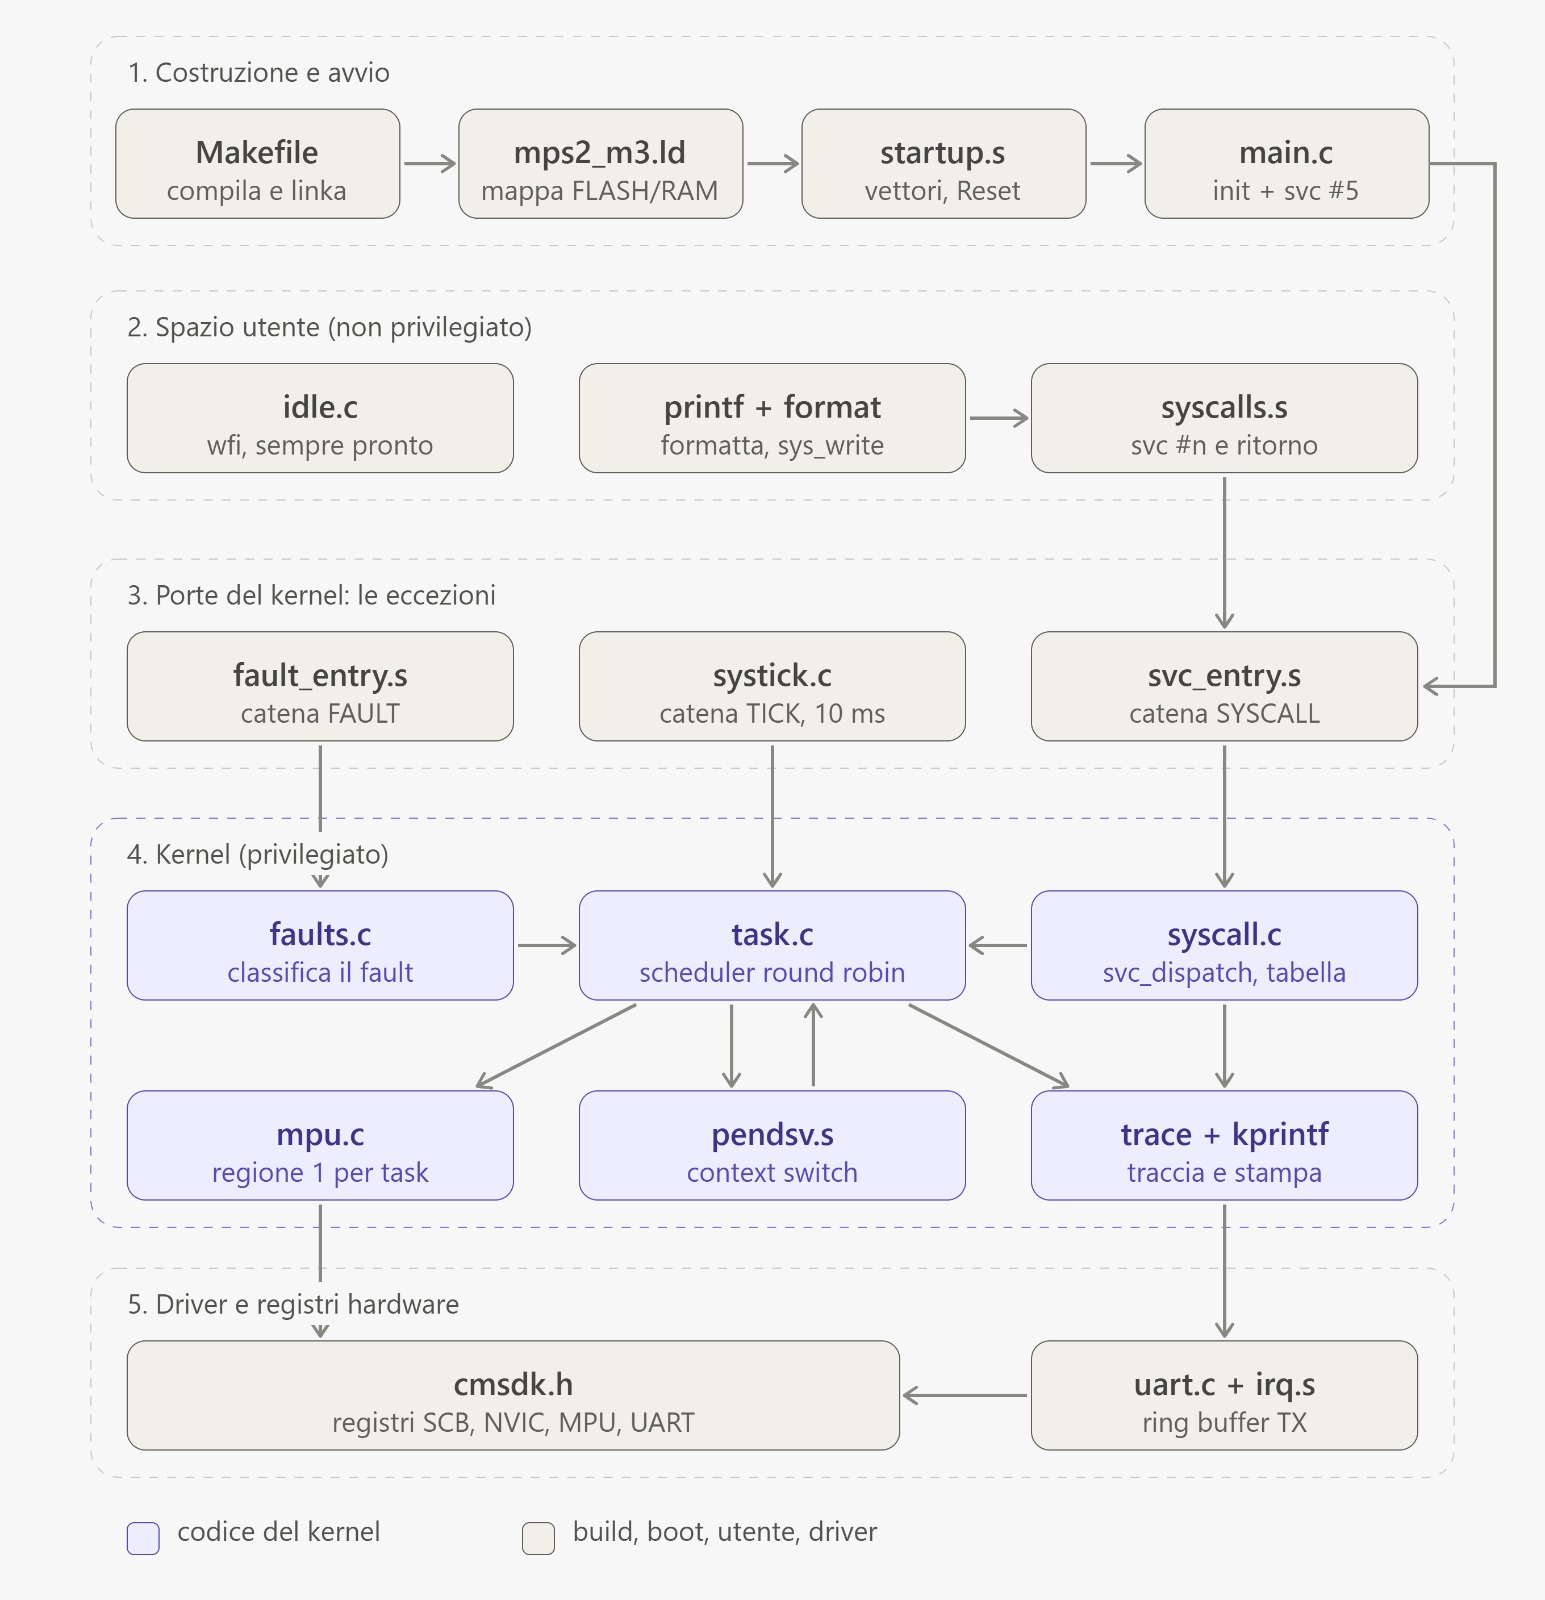
\includegraphics[width=1\textwidth]{contents/images/project/project_base.png}
    \caption{Giulio vaffanculo}
\end{figure}

\subsection{Build e linker}

\paragraph{\texttt{Makefile}} --- Compila ogni \texttt{.c}/\texttt{.s} trovato in \texttt{boot kernel drivers lib src}, linka \texttt{build/scratch-os.axf} e lancia QEMU mps2-an385.
\begin{itemize}
  \item \textbf{Contiene:} variabili \texttt{CC}, \texttt{QUANTUM} (default 5), \texttt{BUILD\_DIR}, \texttt{BIN}, \texttt{IMAGE}, \texttt{IMAGE\_ADDR}, \texttt{IMAGE\_TOOL}, \texttt{PROGRAM\_DIR}, \texttt{SRC\_DIRS}, \texttt{SOURCES}, \texttt{OBJECTS}, \texttt{CFLAGS}, \texttt{LDFLAGS}, \texttt{QEMU}; target \texttt{all}, \texttt{image}, \texttt{run}, \texttt{debug}, \texttt{run-trace}, \texttt{test}, \texttt{clean}
  \item \textbf{Dipende da:} \texttt{scripts/mps2\_m3.ld}; \texttt{tools/mkimage.py} (non presente nella base) e \texttt{programs/} per il target \texttt{image}; \texttt{arm-none-eabi-gcc}, \texttt{qemu-system-arm}, \texttt{python3}; passa \texttt{-DQUANTUM} a \texttt{kernel/task.h}; usa \texttt{-Iinclude} e \texttt{-I.}
  \item \textbf{Usato da:} nessun file (è il punto d'ingresso della build)
  \item \textbf{Tocca:} scrive solo in \texttt{build/} (\texttt{scratch-os.axf}, \texttt{output.map}, \texttt{fs.img} segnaposto); \texttt{clean} fa \texttt{rm -rf build}; QEMU carica \texttt{fs.img} a \texttt{0x00200000}
\end{itemize}

\paragraph{\texttt{scripts/mps2\_m3.ld}} --- Linker script: FLASH a \texttt{0x0} (4M) e RAM a \texttt{0x20000000} (4M); riserva le partizioni di shell e idle e 4 slot da 4 KB per i programmi.
\begin{itemize}
  \item \textbf{Contiene:} \texttt{MEMORY}, \texttt{ENTRY(Reset\_Handler)}, sezioni \texttt{.isr\_vector .text .shell\_stack .shell\_data .shell\_pad .idle\_stack .idle\_data .idle\_pad .program\_slots .data .bss}; simboli \texttt{\_estack}, \texttt{\_sidata}, \texttt{\_sdata}, \texttt{\_edata}, \texttt{\_sbss}, \texttt{\_ebss}, \texttt{\_shell\_*}, \texttt{\_idle\_*}, \texttt{\_\_program\_slot\_*}, \texttt{\_\_fs\_image\_start}, \texttt{\_\_StackLimit}; 4 \texttt{ASSERT}
  \item \textbf{Dipende da:} \texttt{Reset\_Handler} e sezione \texttt{.isr\_vector} (\texttt{boot/startup.s}); \texttt{idle.o} (\texttt{src/idle.c}); \texttt{shell.o} (non presente nella base)
  \item \textbf{Usato da:} \texttt{Makefile} (\texttt{-T}); \texttt{boot/startup.s} usa \texttt{\_estack}, \texttt{\_sidata}, \texttt{\_sdata}, \texttt{\_edata}, \texttt{\_sbss}, \texttt{\_ebss}; \texttt{kernel/task.c} usa \texttt{\_idle\_*} e \texttt{\_\_program\_slots\_start}; \texttt{\_shell\_*}, \texttt{\_\_program\_slot\_N\_*} e \texttt{\_\_fs\_image\_start} non sono usati da nessun file visto
  \item \textbf{Tocca:} solo il layout: stack kernel da 4 KB in cima alla RAM, partizioni da 4 KB allineate (stack da 1 KB in basso), \texttt{.data} caricata in FLASH ed eseguita in RAM
\end{itemize}

\subsection{Boot e definizioni hardware}

\paragraph{\texttt{boot/startup.s}} --- Codice di boot in assembly: tabella dei vettori, \texttt{Reset\_Handler} (costruisce il runtime C e configura la CPU) e \texttt{Default\_Handler}. Alla fine chiama \texttt{main()}.
\begin{itemize}
  \item \textbf{Contiene:} \texttt{isr\_vector} (48 word, sezione \texttt{.isr\_vector}), \texttt{Reset\_Handler} (etichette \texttt{copy\_data}, \texttt{zero\_bss}, \texttt{hang}), \texttt{Default\_Handler}; alias \texttt{.weak}/\texttt{.thumb\_set} di 9 handler di sistema (\texttt{NMI}, \texttt{HardFault}, \texttt{MemManage}, \texttt{BusFault}, \texttt{UsageFault}, \texttt{SVC}, \texttt{DebugMon}, \texttt{PendSV}, \texttt{SysTick}) e di 10 handler di dispositivo (\texttt{UART0RX/TX}, \texttt{UART1RX/TX}, \texttt{UART2RX/TX}, \texttt{TIMER0}, \texttt{TIMER1}, \texttt{DUALTIMER}, \texttt{UARTOVF})
  \item \textbf{Dipende da:} \texttt{\_estack}, \texttt{\_sidata}, \texttt{\_sdata}, \texttt{\_edata}, \texttt{\_sbss}, \texttt{\_ebss} (\texttt{scripts/mps2\_m3.ld}); \texttt{main} (\texttt{src/main.c}); non include \texttt{cmsdk.h} (usa indirizzi scritti a mano)
  \item \textbf{Usato da:} \texttt{scripts/mps2\_m3.ld} (\texttt{ENTRY} e \texttt{.isr\_vector} a \texttt{0x0}); alias sostituiti da \texttt{SVC\_Handler} (\texttt{kernel/svc\_entry.s}), \texttt{PendSV\_Handler} (\texttt{kernel/pendsv.s}), \texttt{SysTick\_Handler} (\texttt{drivers/systick.c}), \texttt{UART0TX\_Handler} (\texttt{drivers/uart.c}), \texttt{MemManage}, \texttt{BusFault}, \texttt{UsageFault} e \texttt{HardFault} (\texttt{kernel/fault\_entry.s}); restano deboli \texttt{NMI}, \texttt{DebugMon}, \texttt{UART0RX}, \texttt{UART1RX/TX}, \texttt{UART2RX/TX}, \texttt{TIMER0}, \texttt{TIMER1}, \texttt{DUALTIMER}, \texttt{UARTOVF}
  \item \textbf{Tocca:} PRIMASK (\texttt{cpsid}/\texttt{cpsie}), SP (= \texttt{\_estack}); copia \texttt{.data} da FLASH a RAM e azzera \texttt{.bss}; VTOR (\texttt{0xE000ED08}), SHCSR (\texttt{0xE000ED24}: abilita MemManage, BusFault, UsageFault), CCR (\texttt{0xE000ED14}: DIV\_0\_TRP), priorità in \texttt{0xE000ED18..23} (fault \texttt{0x00}, SVC \texttt{0x80}, PendSV e SysTick \texttt{0xE0}); usa r0--r3
\end{itemize}

\paragraph{\texttt{include/cmsdk.h}} --- Definizioni dei registri di mps2-an385: struct sovrapposte ai periferici (SysTick, NVIC, SCB, MPU, UART0--2, TIMER0--1, WDOG, GPIO0, FPGAIO), con macro dei bit, costanti \texttt{*\_IRQn} e \texttt{\_Static\_assert} sugli offset; molte macro non sono usate da nessun file visto.
\begin{itemize}
  \item \textbf{Dipende da:} \texttt{stdint.h}, \texttt{stddef.h}. \textbf{Usato da:} \texttt{drivers/systick.c}, \texttt{drivers/uart.c}, \texttt{kernel/mpu.c}, \texttt{kernel/faults.c}, \texttt{kernel/task.c}. \textbf{Tocca:} niente (solo definizioni)
\end{itemize}

\subsection{Applicazione di base (\texttt{src})}

\paragraph{\texttt{src/main.c}} --- Entry point del kernel: inizializza UART, SysTick e MPU, poi lancia i task con \texttt{svc \#5} (\texttt{SYS\_START\_TASKS}). Non ritorna mai.
\begin{itemize}
  \item \textbf{Contiene:} \texttt{main()}
  \item \textbf{Dipende da:} \texttt{drivers/uart.h} (\texttt{uart\_init}), \texttt{drivers/systick.h} (\texttt{systick\_init}), \texttt{kernel/kprintf.h} (\texttt{kprintf}), \texttt{kernel/mpu.h} (\texttt{mpu\_init}); non include \texttt{lib/syscalls.h}: il numero 5 è scritto a mano e va tenuto coerente con \texttt{SYS\_START\_TASKS}; l'\texttt{svc} è servita da \texttt{kernel/svc\_entry.s} e \texttt{kernel/syscall.c}
  \item \textbf{Usato da:} \texttt{Reset\_Handler} in \texttt{boot/startup.s} (\texttt{bl main})
  \item \textbf{Tocca:} indirettamente UART, SysTick (tick da 10 ms) e MPU tramite le init; \texttt{svc \#5} genera l'eccezione SVC con clobber \texttt{memory}
\end{itemize}

\paragraph{\texttt{src/tasks.h}} --- Dichiara l'idle task, l'unico avviato dalla base.
\begin{itemize}
  \item \textbf{Contiene:} guard \texttt{TASKS\_H}, prototipo \texttt{idle\_task()}
  \item \textbf{Dipende da:} niente
  \item \textbf{Usato da:} \texttt{src/idle.c} (include); \texttt{kernel/task.c} (include, usa \texttt{idle\_task} come \texttt{.entry} dell'idle TCB)
  \item \textbf{Tocca:} niente (solo dichiarazione)
\end{itemize}

\paragraph{\texttt{src/idle.c}} --- Idle task: loop infinito con \texttt{wfi}, gira quando nessun task è READY; non privilegiato, con stack e partizione MPU propri.
\begin{itemize}
  \item \textbf{Contiene:} \texttt{idle\_task()}
  \item \textbf{Dipende da:} \texttt{src/tasks.h}; istruzione \texttt{wfi} (asm inline); \texttt{scripts/mps2\_m3.ld} lo mette nelle sezioni \texttt{.idle\_*} tramite il nome \texttt{idle.o}
  \item \textbf{Usato da:} \texttt{kernel/task.c} (\texttt{tasks[IDLE\_TASK\_INDEX].entry})
  \item \textbf{Tocca:} nessuna variabile; \texttt{wfi} ferma la CPU fino al prossimo interrupt (SysTick); usa lo stack da 1 KB della partizione idle
\end{itemize}

\subsection{Driver}

\paragraph{\texttt{drivers/systick.h}} --- Interfaccia del driver SysTick: il timer del core usato come tick di sistema da 10 ms.
\begin{itemize}
  \item \textbf{Contiene:} guard \texttt{SYSTICK\_H}, macro \texttt{TICK\_MS} (10), prototipi \texttt{systick\_init()}, \texttt{SysTick\_Handler()}, \texttt{systick\_uptime\_ms()}
  \item \textbf{Dipende da:} \texttt{stdint.h}
  \item \textbf{Usato da:} \texttt{src/main.c}, \texttt{drivers/systick.c}, \texttt{kernel/syscall.c} (include)
  \item \textbf{Tocca:} niente (solo dichiarazioni)
\end{itemize}

\paragraph{\texttt{drivers/systick.c}} --- Configura SysTick a 25 MHz per un'eccezione ogni 10 ms. L'handler aggiorna l'uptime e avvisa lo scheduler.
\begin{itemize}
  \item \textbf{Contiene:} \texttt{CPU\_CLOCK\_HZ}, \texttt{uptime\_ms} (static volatile), \texttt{systick\_init()}, \texttt{SysTick\_Handler()}, \texttt{systick\_uptime\_ms()}
  \item \textbf{Dipende da:} \texttt{drivers/systick.h}; \texttt{cmsdk.h} (\texttt{SysTick->LOAD/VAL/CTRL}, \texttt{SysTick\_CTRL\_*}); \texttt{kernel/task.h} (\texttt{task\_increment\_tick}, definita in \texttt{kernel/task.c})
  \item \textbf{Usato da:} \texttt{src/main.c} (\texttt{systick\_init}); \texttt{kernel/syscall.c} (\texttt{systick\_uptime\_ms}); \texttt{SysTick\_Handler} sostituisce l'alias debole di \texttt{boot/startup.s} (vettore 15)
  \item \textbf{Tocca:} SysTick \texttt{LOAD} (249999), \texttt{VAL} (0), \texttt{CTRL} (ENABLE, TICKINT, CLKSOURCE); variabile \texttt{uptime\_ms}
\end{itemize}

\paragraph{\texttt{drivers/uart.h}} --- Interfaccia del driver UART0: invio polled o con ring buffer e interrupt, ricezione solo polled.
\begin{itemize}
  \item \textbf{Contiene:} guard \texttt{UART\_H}, prototipi \texttt{uart\_init}, \texttt{uart\_putc\_polled}, \texttt{uart\_getc\_polled}, \texttt{uart\_write}, \texttt{UART0TX\_Handler}
  \item \textbf{Dipende da:} niente
  \item \textbf{Usato da:} \texttt{src/main.c}, \texttt{drivers/uart.c}, \texttt{kernel/kprintf.c}, \texttt{kernel/syscall.c} (include)
  \item \textbf{Tocca:} niente (solo dichiarazioni)
\end{itemize}

\paragraph{\texttt{drivers/uart.c}} --- Driver UART0: invio con ring buffer da 64 byte pilotato dall'interrupt TX, più invio e ricezione polled.
\begin{itemize}
  \item \textbf{Contiene:} \texttt{TX\_BUF\_SIZE}, \texttt{tx\_buf}, \texttt{tx\_head}, \texttt{tx\_tail}, \texttt{tx\_busy}, \texttt{tx\_empty}, \texttt{tx\_full}, \texttt{tx\_pop}, \texttt{uart\_init}, \texttt{uart\_putc\_polled}, \texttt{uart\_getc\_polled}, \texttt{uart\_write}, \texttt{UART0TX\_Handler}
  \item \textbf{Dipende da:} \texttt{drivers/uart.h}; \texttt{cmsdk.h} (\texttt{CMSDK\_UART0}, \texttt{UART\_CTRL\_*}, \texttt{UART\_STATE\_*}, \texttt{UART\_INT\_TX}, \texttt{NVIC}, \texttt{UART0TX\_IRQn}); \texttt{kernel/irq.h} (\texttt{irq\_save}, \texttt{irq\_restore}, implementate in \texttt{kernel/irq.s})
  \item \textbf{Usato da:} \texttt{src/main.c} (\texttt{uart\_init}); \texttt{kernel/kprintf.c} (\texttt{uart\_putc\_polled}); \texttt{kernel/syscall.c} (\texttt{uart\_write}, \texttt{uart\_getc\_polled}); \texttt{UART0TX\_Handler} sostituisce l'alias debole di \texttt{boot/startup.s} (vettore 17)
  \item \textbf{Tocca:} UART0 \texttt{BAUDDIV} (16), \texttt{CTRL} (TXEN, RXEN, TXIRQEN), \texttt{DATA}, \texttt{INTSTATUS}; NVIC \texttt{IPR} (0xC0) e \texttt{ISER} per UART0TX; PRIMASK (via \texttt{irq\_save}); globali \texttt{tx\_buf}, \texttt{tx\_head}, \texttt{tx\_tail}, \texttt{tx\_busy}
\end{itemize}

\subsection{Kernel}

\paragraph{\texttt{kernel/task.h}} --- Interfaccia dello scheduler: TCB, tabella dei task, stati e funzioni del kernel (round robin preemptive con time slice \texttt{QUANTUM}).
\begin{itemize}
  \item \textbf{Contiene:} guard \texttt{TASK\_H}, \texttt{QUANTUM} (default 5, ridefinito da \texttt{-DQUANTUM}), \texttt{enum task\_state}, \texttt{struct tcb} (\texttt{sp} deve restare il primo campo), \texttt{PROGRAM\_SLOT\_COUNT}, \texttt{SHELL\_TASK\_INDEX}, \texttt{PROGRAM\_TASK\_FIRST}, \texttt{IDLE\_TASK\_INDEX}, \texttt{NUM\_TASKS}; extern \texttt{tasks}, \texttt{tcb\_current}, \texttt{tick\_count}; prototipi \texttt{task\_start\_first}, \texttt{task\_increment\_tick}, \texttt{task\_request\_switch}, \texttt{task\_block\_until}, \texttt{task\_finish\_current}, \texttt{task\_project\_configure}, \texttt{task\_configure\_shell}, \texttt{task\_program\_create}, \texttt{task\_program\_slot\_free}, \texttt{task\_wait\_program}, \texttt{task\_fault\_current}, \texttt{task\_current\_is\_program}, \texttt{task\_switch\_context}
  \item \textbf{Dipende da:} \texttt{stdint.h}; definizioni in \texttt{kernel/task.c}; \texttt{QUANTUM} dal \texttt{Makefile}
  \item \textbf{Usato da:} \texttt{drivers/systick.c}, \texttt{kernel/syscall.c}, \texttt{kernel/task.c}, \texttt{kernel/faults.c}, \texttt{kernel/trace.c} (include); \texttt{kernel/pendsv.s} (non lo include, ma assume \texttt{sp} a offset 0 e usa \texttt{tcb\_current})
  \item \textbf{Tocca:} niente (solo dichiarazioni)
\end{itemize}

\paragraph{\texttt{kernel/task.c}} --- Scheduler round robin: tabella dei task, frame iniziali, tick, scelta del prossimo task, slot dei programmi caricati (id con generazione, attesa, fault). Gira privilegiato dentro SVCall, SysTick e PendSV.
\begin{itemize}
  \item \textbf{Contiene:} \texttt{tasks[]}, \texttt{tcb\_current}, \texttt{tick\_count}, \texttt{quantum\_left}, \texttt{rr\_last}, \texttt{program\_names}, \texttt{generations}, \texttt{completed\_id}, \texttt{completed\_status}; \texttt{partition\_init}, \texttt{task\_init\_stack}, \texttt{task\_project\_configure} (weak), \texttt{task\_configure\_shell}, \texttt{task\_start\_first}, \texttt{task\_request\_switch}, \texttt{task\_increment\_tick}, \texttt{task\_block\_until}, \texttt{program\_index}, \texttt{task\_current\_is\_program}, \texttt{task\_program\_slot\_free}, \texttt{task\_program\_create}, \texttt{task\_wait\_program}, \texttt{complete\_program}, \texttt{task\_finish\_current}, \texttt{task\_fault\_current}, \texttt{task\_switch\_context}
  \item \textbf{Dipende da:} \texttt{cmsdk.h} (\texttt{SCB->ICSR}, \texttt{SCB\_ICSR\_PENDSVSET}); \texttt{kernel/task.h}; \texttt{kernel/mpu.h} (\texttt{mpu\_set\_task\_region}); \texttt{kernel/kprintf.h}; \texttt{kernel/trace.h} (\texttt{trace\_record\_switch}); \texttt{src/tasks.h} (\texttt{idle\_task}); \texttt{lib/syscalls.h} (\texttt{task\_exit}, in \texttt{lib/syscalls.s}); simboli del linker \texttt{\_idle\_part\_start}, \texttt{\_idle\_stack\_top}, \texttt{\_idle\_part\_end}, \texttt{\_idle\_data\_*}, \texttt{\_\_program\_slots\_start}; definizione forte di \texttt{task\_project\_configure} (shell degli studenti, non presente nella base)
  \item \textbf{Usato da:} \texttt{drivers/systick.c} (\texttt{task\_increment\_tick}); \texttt{kernel/syscall.c} (\texttt{task\_start\_first}, \texttt{task\_request\_switch}, \texttt{task\_block\_until}, \texttt{task\_finish\_current}, \texttt{task\_wait\_program}, \texttt{tcb\_current}, \texttt{tick\_count}); \texttt{kernel/pendsv.s} (\texttt{tcb\_current}, \texttt{task\_switch\_context}); \texttt{kernel/faults.c} (\texttt{task\_current\_is\_program}, \texttt{task\_fault\_current}); \texttt{kernel/trace.c} (\texttt{tasks}, \texttt{tick\_count})
  \item \textbf{Tocca:} i globali elencati; \texttt{ICSR.PENDSVSET}; MPU regione 1 a ogni switch; PSP e \texttt{CONTROL.nPRIV} (una volta, in \texttt{task\_start\_first}); copia i dati iniziali di shell e idle; scrive il frame iniziale (xPSR, pc, lr = \texttt{task\_exit}, r0--r12) sullo stack di ogni task; stampa con \texttt{kprintf}; scrive nel r0 salvato di un task in attesa (\texttt{wait\_result})
\end{itemize}

\paragraph{\texttt{kernel/syscall.h}} --- Lato kernel delle system call: dichiara \texttt{svc\_dispatch()}.
\begin{itemize}
  \item \textbf{Contiene:} guard \texttt{SYSCALL\_H}, prototipo \texttt{svc\_dispatch()}
  \item \textbf{Dipende da:} \texttt{stdint.h}
  \item \textbf{Usato da:} \texttt{kernel/syscall.c} (include); \texttt{kernel/svc\_entry.s} (\texttt{bl svc\_dispatch})
  \item \textbf{Tocca:} niente (solo dichiarazione)
\end{itemize}

\paragraph{\texttt{kernel/syscall.c}} --- Smista \texttt{svc \#n} leggendo \texttt{n} dal byte prima del pc salvato, esegue il servizio dalla tabella e scrive il risultato nel r0 salvato. \texttt{SYS\_START\_TASKS} è gestito a parte. \texttt{TABLE\_SIZE} vale 15 (il commento dice 11); i servizi 11--13 non hanno voce e rispondono \texttt{-1}.
\begin{itemize}
  \item \textbf{Contiene:} \texttt{syscall\_fn}, \texttt{in\_range}, \texttt{sys\_write\_impl}, \texttt{sys\_read\_impl}, \texttt{sys\_uptime\_impl}, \texttt{sys\_yield\_impl}, \texttt{sys\_delay\_impl}, \texttt{sys\_delay\_until\_impl}, \texttt{sys\_exit\_impl}, \texttt{sys\_tick\_count\_impl}, \texttt{sys\_trace\_dump\_impl}, \texttt{sys\_program\_wait\_impl}, \texttt{table}, \texttt{TABLE\_SIZE}, \texttt{EXC\_RETURN\_PSP\_BIT}, \texttt{svc\_dispatch}
  \item \textbf{Dipende da:} \texttt{kernel/syscall.h}; \texttt{lib/syscalls.h} (\texttt{SYS\_*}); \texttt{drivers/uart.h} (\texttt{uart\_write}, \texttt{uart\_getc\_polled}); \texttt{drivers/systick.h} (\texttt{systick\_uptime\_ms}); \texttt{kernel/task.h} (\texttt{tcb\_current}, \texttt{tick\_count}, \texttt{task\_request\_switch}, \texttt{task\_block\_until}, \texttt{task\_finish\_current}, \texttt{task\_start\_first}, \texttt{task\_wait\_program}, campi \texttt{part\_start}/\texttt{part\_end}); \texttt{kernel/trace.h} (\texttt{trace\_print})
  \item \textbf{Usato da:} \texttt{kernel/svc\_entry.s} (chiama \texttt{svc\_dispatch})
  \item \textbf{Tocca:} \texttt{frame[0]} (r0 salvato del chiamante); legge \texttt{frame[6]} e il byte a \texttt{pc-2}; legge PSP (\texttt{sys\_program\_wait\_impl}); scrive \texttt{*last\_wake} nella partizione del task; stato dei task solo tramite le funzioni di \texttt{kernel/task.c}
\end{itemize}

\paragraph{\texttt{kernel/svc\_entry.s}} --- \texttt{SVC\_Handler}: sceglie MSP o PSP dal bit 2 di EXC\_RETURN, chiama \texttt{svc\_dispatch(frame, exc\_return)} e termina l'eccezione con il valore restituito.
\begin{itemize}
  \item \textbf{Contiene:} \texttt{SVC\_Handler}
  \item \textbf{Dipende da:} \texttt{svc\_dispatch} (\texttt{kernel/syscall.c})
  \item \textbf{Usato da:} vettore 11 di \texttt{boot/startup.s} (sostituisce l'alias debole); entrato da ogni \texttt{svc} di \texttt{lib/syscalls.s} e di \texttt{src/main.c}
  \item \textbf{Tocca:} legge \texttt{lr}, MSP e PSP; usa r0 e r1; non scrive sullo stack; \texttt{bx r0} con EXC\_RETURN
\end{itemize}

\paragraph{\texttt{kernel/pendsv.s}} --- \texttt{PendSV\_Handler}: il context switch. Salva r4--r11 sullo stack del task, chiama \texttt{task\_switch\_context()}, ripristina r4--r11 del nuovo task e rientra con \texttt{0xFFFFFFFD}.
\begin{itemize}
  \item \textbf{Contiene:} \texttt{PendSV\_Handler}, \texttt{.ltorg}
  \item \textbf{Dipende da:} \texttt{tcb\_current} e \texttt{task\_switch\_context} (\texttt{kernel/task.c}, dichiarati in \texttt{kernel/task.h}); campo \texttt{sp} a offset 0 di \texttt{struct tcb}
  \item \textbf{Usato da:} vettore 14 di \texttt{boot/startup.s} (sostituisce l'alias debole); reso pending da \texttt{task\_request\_switch()} (\texttt{kernel/task.c}), chiamata da SysTick e da \texttt{kernel/syscall.c}
  \item \textbf{Tocca:} PSP; r0--r2 e r4--r11; 8 word sullo stack del task; \texttt{tcb\_current->sp}; priorità \texttt{0xE0} impostata in \texttt{boot/startup.s}
\end{itemize}

\paragraph{\texttt{kernel/mpu.h}} --- Interfaccia dell'MPU: regione 0 = FLASH in sola lettura, regione 1 = partizione del task corrente.
\begin{itemize}
  \item \textbf{Contiene:} guard \texttt{MPU\_H}, prototipi \texttt{mpu\_init()}, \texttt{mpu\_set\_task\_region()}
  \item \textbf{Dipende da:} \texttt{stdint.h}
  \item \textbf{Usato da:} \texttt{src/main.c} (\texttt{mpu\_init}), \texttt{kernel/mpu.c}, \texttt{kernel/task.c} (\texttt{mpu\_set\_task\_region}, da \texttt{task\_start\_first} e \texttt{task\_switch\_context})
  \item \textbf{Tocca:} niente (solo dichiarazioni)
\end{itemize}

\paragraph{\texttt{kernel/mpu.c}} --- Configura la regione 0 (FLASH, 4 MB, sola lettura) e abilita l'MPU con PRIVDEFENA; \texttt{mpu\_set\_task\_region} punta la regione 1 alla partizione del task (RW, XN salvo \texttt{executable}).
\begin{itemize}
  \item \textbf{Contiene:} \texttt{mpu\_init}, \texttt{mpu\_set\_task\_region}
  \item \textbf{Dipende da:} \texttt{stdint.h}; \texttt{kernel/mpu.h}; \texttt{cmsdk.h} (\texttt{MPU->RBAR/RASR/CTRL}, \texttt{MPU\_RBAR\_VALID}, \texttt{MPU\_RASR\_*}, \texttt{MPU\_AP\_*}, \texttt{MPU\_CTRL\_*}); \texttt{\_\_builtin\_ctz}
  \item \textbf{Usato da:} \texttt{src/main.c} (\texttt{mpu\_init}); \texttt{kernel/task.c} (\texttt{mpu\_set\_task\_region})
  \item \textbf{Tocca:} MPU \texttt{RBAR} e \texttt{RASR} (regioni 0 e 1), \texttt{CTRL} (= 5); istruzioni \texttt{dsb} e \texttt{isb}
\end{itemize}

\paragraph{\texttt{kernel/fault\_entry.s}} --- Entry point dei fault: una macro \texttt{FAULT} genera quattro handler che passano a C il tipo di fault (r0) e EXC\_RETURN (r1).
\begin{itemize}
  \item \textbf{Contiene:} macro \texttt{FAULT}; \texttt{MemManage\_Handler} (1), \texttt{BusFault\_Handler} (2), \texttt{UsageFault\_Handler} (3), \texttt{HardFault\_Handler} (4)
  \item \textbf{Dipende da:} \texttt{fault\_dispatch} (\texttt{kernel/faults.c})
  \item \textbf{Usato da:} vettori 3--6 di \texttt{boot/startup.s} (sostituiscono gli alias deboli); i fault configurabili sono abilitati da SHCSR in \texttt{Reset\_Handler}
  \item \textbf{Tocca:} r0 e r1; salta con \texttt{b} (non \texttt{bl}), quindi \texttt{lr} resta EXC\_RETURN e il ritorno di \texttt{fault\_dispatch} termina l'eccezione; nessuno stack
\end{itemize}

\paragraph{\texttt{kernel/faults.c}} --- Classifica il fault leggendo CFSR. Se viene da un programma caricato e non è un errore di stacking, stampa, cancella CFSR e termina il task; altrimenti stampa e si ferma.
\begin{itemize}
  \item \textbf{Contiene:} \texttt{EXC\_RETURN\_PSP\_BIT}, \texttt{BUS\_STACK\_ERRORS}, \texttt{halt} (static), \texttt{fault\_dispatch}
  \item \textbf{Dipende da:} \texttt{cmsdk.h} (\texttt{SCB->CFSR/HFSR/MMFAR}, \texttt{SCB\_CFSR\_MSTKERR}, \texttt{SCB\_CFSR\_MUNSTKERR}, \texttt{SCB\_CFSR\_MMARVALID}); \texttt{kernel/kprintf.h}; \texttt{kernel/task.h} (\texttt{task\_current\_is\_program}, \texttt{task\_fault\_current}, in \texttt{kernel/task.c})
  \item \textbf{Usato da:} \texttt{kernel/fault\_entry.s} (salto a \texttt{fault\_dispatch})
  \item \textbf{Tocca:} SCB \texttt{CFSR} (riscritto per azzerare i flag); legge \texttt{HFSR} e \texttt{MMFAR}; UART via \texttt{kprintf}; stato del task corrente via \texttt{task\_fault\_current}; nel caso irrecuperabile resta in un ciclo infinito
\end{itemize}

\paragraph{\texttt{kernel/irq.h}} --- Interfaccia per mascherare e riabilitare gli interrupt attorno a una sezione critica.
\begin{itemize}
  \item \textbf{Contiene:} guard \texttt{IRQ\_H}, prototipi \texttt{irq\_save()}, \texttt{irq\_restore()}
  \item \textbf{Dipende da:} \texttt{stdint.h}; implementazione in \texttt{kernel/irq.s}
  \item \textbf{Usato da:} \texttt{drivers/uart.c} (include)
  \item \textbf{Tocca:} niente (solo dichiarazioni)
\end{itemize}

\paragraph{\texttt{kernel/irq.s}} --- \texttt{irq\_save} legge PRIMASK e maschera gli interrupt; \texttt{irq\_restore} rimette il valore salvato.
\begin{itemize}
  \item \textbf{Contiene:} \texttt{irq\_save}, \texttt{irq\_restore}
  \item \textbf{Dipende da:} niente (solo istruzioni \texttt{mrs}, \texttt{msr}, \texttt{cpsid})
  \item \textbf{Usato da:} \texttt{drivers/uart.c} (\texttt{uart\_write}), tramite \texttt{kernel/irq.h}
  \item \textbf{Tocca:} PRIMASK; r0 (valore di ritorno e argomento); nessuno stack
\end{itemize}

\paragraph{\texttt{kernel/kprintf.h}} --- Interfaccia della print del kernel, che usa la UART in polling e funziona anche dentro un fault handler.
\begin{itemize}
  \item \textbf{Contiene:} guard \texttt{KPRINTF\_H}, prototipo \texttt{kprintf()}
  \item \textbf{Dipende da:} niente
  \item \textbf{Usato da:} \texttt{src/main.c}, \texttt{kernel/kprintf.c}, \texttt{kernel/faults.c}, \texttt{kernel/trace.c}, \texttt{kernel/task.c}
  \item \textbf{Tocca:} niente (solo dichiarazione)
\end{itemize}

\paragraph{\texttt{kernel/kprintf.c}} --- \texttt{kprintf} formatta con \texttt{vformat} e invia ogni carattere con \texttt{uart\_putc\_polled}.
\begin{itemize}
  \item \textbf{Contiene:} \texttt{kprintf\_out} (static), \texttt{kprintf}
  \item \textbf{Dipende da:} \texttt{kernel/kprintf.h}; \texttt{lib/format.h} (\texttt{vformat}, e \texttt{stdarg.h}); \texttt{drivers/uart.h} (\texttt{uart\_putc\_polled})
  \item \textbf{Usato da:} \texttt{src/main.c}, \texttt{kernel/faults.c}, \texttt{kernel/trace.c}, \texttt{kernel/task.c}
  \item \textbf{Tocca:} nessun globale; UART0 \texttt{DATA} (attende \texttt{TXBF}) tramite \texttt{uart\_putc\_polled}
\end{itemize}

\paragraph{\texttt{kernel/trace.h}} --- Interfaccia della traccia dello scheduler: registra ogni cambio di task e lo stampa con un diagramma di Gantt.
\begin{itemize}
  \item \textbf{Contiene:} guard \texttt{TRACE\_H}, prototipi \texttt{trace\_record\_switch()}, \texttt{trace\_print()}
  \item \textbf{Dipende da:} \texttt{stdint.h}
  \item \textbf{Usato da:} \texttt{kernel/trace.c}, \texttt{kernel/syscall.c} (\texttt{trace\_print}), \texttt{kernel/task.c} (\texttt{trace\_record\_switch}, da \texttt{task\_switch\_context})
  \item \textbf{Tocca:} niente (solo dichiarazioni)
\end{itemize}

\paragraph{\texttt{kernel/trace.c}} --- Buffer ad anello da 64 record (tick, task di partenza, task di arrivo). \texttt{trace\_print} stampa il formato \texttt{TRACE BEGIN/END} e poi il Gantt.
\begin{itemize}
  \item \textbf{Contiene:} \texttt{struct trace\_record}, \texttt{TRACE\_SIZE}, \texttt{buffer}, \texttt{count}, \texttt{trace\_record\_switch}, \texttt{stored}, \texttt{oldest\_plus}, \texttt{owner\_at}, \texttt{GANTT\_COLUMNS}, \texttt{draw\_gantt}, \texttt{trace\_print}
  \item \textbf{Dipende da:} \texttt{kernel/trace.h}; \texttt{kernel/task.h} (\texttt{tick\_count}, \texttt{tasks}, \texttt{NUM\_TASKS}, definiti in \texttt{kernel/task.c}); \texttt{kernel/kprintf.h}
  \item \textbf{Usato da:} \texttt{kernel/syscall.c} (\texttt{trace\_print}, per \texttt{SYS\_TRACE\_DUMP}); \texttt{kernel/task.c} (\texttt{trace\_record\_switch})
  \item \textbf{Tocca:} globali \texttt{buffer} e \texttt{count} (nessuna protezione: PendSV e SVCall non si interrompono); legge \texttt{tick\_count} e i nomi in \texttt{tasks[]}; UART via \texttt{kprintf}
\end{itemize}

\subsection{Libreria lato utente (\texttt{lib})}

\paragraph{\texttt{lib/format.h}} --- Interfaccia della formattazione testo: numeri e stringa di formato diventano caratteri passati a una funzione \texttt{out} del chiamante.
\begin{itemize}
  \item \textbf{Contiene:} guard \texttt{FORMAT\_H}, prototipi \texttt{utoa\_dec}, \texttt{utoa\_hex}, \texttt{vformat}
  \item \textbf{Dipende da:} \texttt{stdarg.h}, \texttt{stdint.h}
  \item \textbf{Usato da:} \texttt{lib/format.c}, \texttt{lib/printf.c}, \texttt{kernel/kprintf.c}
  \item \textbf{Tocca:} niente (solo dichiarazioni)
\end{itemize}

\paragraph{\texttt{lib/format.c}} --- Implementa \texttt{utoa\_dec}, \texttt{utoa\_hex} e \texttt{vformat} (conversioni \texttt{c s d u x} e il segno di percentuale, senza larghezza né precisione).
\begin{itemize}
  \item \textbf{Contiene:} \texttt{utoa\_base} (static), \texttt{utoa\_dec}, \texttt{utoa\_hex}, \texttt{put\_string} (static), \texttt{vformat}
  \item \textbf{Dipende da:} \texttt{lib/format.h}; la funzione \texttt{out} e il \texttt{ctx} ricevuti dal chiamante
  \item \textbf{Usato da:} \texttt{lib/printf.c} e \texttt{kernel/kprintf.c} (\texttt{vformat})
  \item \textbf{Tocca:} nessuno stato globale né registri hardware; solo i buffer del chiamante e il proprio stack (\texttt{tmp[10]}, \texttt{num[12]})
\end{itemize}

\paragraph{\texttt{lib/printf.h}} --- Interfaccia dell'output e delle attese lato utente, costruite solo sulle system call.
\begin{itemize}
  \item \textbf{Contiene:} guard \texttt{PRINTF\_H}, prototipi \texttt{write\_all}, \texttt{printf}, \texttt{sleep\_ms}, \texttt{spin\_ticks}
  \item \textbf{Dipende da:} \texttt{stdint.h}
  \item \textbf{Usato da:} \texttt{lib/printf.c}; shell e programmi (non presenti nella base)
  \item \textbf{Tocca:} niente (solo dichiarazioni)
\end{itemize}

\paragraph{\texttt{lib/printf.c}} --- Output non privilegiato: \texttt{printf} formatta con \texttt{vformat} in un buffer da 64 byte e lo invia con \texttt{sys\_write}. Include \texttt{sleep\_ms} e \texttt{spin\_ticks}.
\begin{itemize}
  \item \textbf{Contiene:} \texttt{PRINTF\_BUF\_SIZE}, \texttt{write\_all}, \texttt{struct printf\_ctx}, \texttt{printf\_out} (static), \texttt{printf}, \texttt{sleep\_ms}, \texttt{spin\_ticks}
  \item \textbf{Dipende da:} \texttt{stdarg.h}; \texttt{lib/printf.h}; \texttt{lib/format.h} (\texttt{vformat}); \texttt{lib/syscalls.h} (\texttt{sys\_write}, \texttt{sys\_uptime}, \texttt{task\_tick\_count}, in \texttt{lib/syscalls.s}); istruzione \texttt{wfi}
  \item \textbf{Usato da:} nessun file della base; pensato per shell e programmi (non presenti)
  \item \textbf{Tocca:} nessun globale; \texttt{struct printf\_ctx} (circa 72 byte) sullo stack del chiamante; \texttt{wfi}; indirettamente SVC tramite le system call
\end{itemize}

\paragraph{\texttt{lib/syscalls.h}} --- Header condiviso tra kernel e applicazioni: numeri dei servizi e prototipi delle system call.
\begin{itemize}
  \item \textbf{Contiene:} guard \texttt{SYSCALLS\_H}, macro \texttt{SYS\_WRITE} (1) \ldots{} \texttt{SYS\_PROGRAM\_WAIT} (14), con \texttt{SYS\_START\_TASKS} = 5; prototipi \texttt{sys\_write}, \texttt{sys\_read}, \texttt{sys\_uptime}, \texttt{sys\_exit}, \texttt{task\_yield}, \texttt{task\_delay}, \texttt{task\_delay\_until}, \texttt{task\_tick\_count}, \texttt{trace\_dump}, \texttt{sys\_image\_count}, \texttt{sys\_image\_name}, \texttt{sys\_program\_run}, \texttt{sys\_program\_wait}, \texttt{task\_exit}
  \item \textbf{Dipende da:} \texttt{stdint.h}
  \item \textbf{Usato da:} \texttt{lib/printf.c}, \texttt{kernel/syscall.c}, \texttt{kernel/task.c} (include); \texttt{lib/syscalls.s} e \texttt{src/main.c} ne ripetono a mano i numeri
  \item \textbf{Tocca:} niente (solo dichiarazioni)
\end{itemize}

\paragraph{\texttt{lib/syscalls.s}} --- Lato utente delle system call: ogni funzione fa \texttt{svc \#n} e poi \texttt{bx lr}; argomenti in r0--r2, risultato in r0. Non c'è stub per \texttt{svc \#5} (lo scrive \texttt{main.c}).
\begin{itemize}
  \item \textbf{Contiene:} \texttt{sys\_write}, \texttt{sys\_read}, \texttt{sys\_uptime}, \texttt{sys\_exit}, \texttt{task\_yield}, \texttt{task\_delay}, \texttt{task\_delay\_until}, \texttt{trace\_dump}, \texttt{task\_tick\_count}, \texttt{sys\_image\_count}, \texttt{sys\_image\_name}, \texttt{sys\_program\_run}, \texttt{sys\_program\_wait}, \texttt{task\_exit}
  \item \textbf{Dipende da:} numeri \texttt{svc} scritti a mano e coerenti con \texttt{lib/syscalls.h}; \texttt{SVC\_Handler} (\texttt{kernel/svc\_entry.s}) e \texttt{svc\_dispatch} (\texttt{kernel/syscall.c}); \texttt{task\_exit} chiama \texttt{sys\_exit}
  \item \textbf{Usato da:} \texttt{lib/printf.c} (\texttt{sys\_write}, \texttt{sys\_uptime}, \texttt{task\_tick\_count}); \texttt{kernel/task.c} usa l'indirizzo di \texttt{task\_exit} come lr iniziale di ogni task
  \item \textbf{Tocca:} nessun registro scritto direttamente; \texttt{svc} fa salvare r0--r3, r12, lr, pc, xPSR sullo stack e il kernel scrive il risultato nel r0 salvato; \texttt{sys\_exit} e \texttt{task\_exit} non tornano
\end{itemize}

\subsection{Programmi}

\paragraph{\texttt{programs/README.md}} --- Nota di una riga: la cartella accoglie sorgenti e input dei programmi caricabili, passata a \texttt{tools/mkimage.py}.
\begin{itemize}
  \item \textbf{Contiene:} solo testo Markdown
  \item \textbf{Dipende da:} \texttt{tools/mkimage.py} (scritto dagli studenti, non presente nella base)
  \item \textbf{Usato da:} \texttt{Makefile} (\texttt{PROGRAM\_DIR}, target \texttt{image}); non è in \texttt{SRC\_DIRS}, quindi \texttt{make} non la compila
  \item \textbf{Tocca:} niente
\end{itemize}

\subsection{Mappa finale delle dipendenze}

{\footnotesize
\begin{verbatim}
    DIPENDENZE (file -> file; * = non presente nella base)
    Makefile     -> mps2_m3.ld, tools/mkimage.py*, programs/*
    mps2_m3.ld   -> startup.s (Reset_Handler, .isr_vector), idle.o, shell.o*
    startup.s    -> mps2_m3.ld (simboli), main.c, svc_entry.s, pendsv.s, fault_entry.s, systick.c, uart.c
    main.c       -> uart.h, systick.h, kprintf.h, mpu.h  (svc #5 scritto a mano, = SYS_START_TASKS)
    idle.c       -> src/tasks.h  |  irq.s -> nessuno  |  format.c -> format.h
    systick.c    -> systick.h, cmsdk.h, kernel/task.h  |  uart.c -> uart.h, cmsdk.h, irq.h
    task.c       -> kernel/task.h, cmsdk.h, mpu.h, kprintf.h, trace.h, src/tasks.h, lib/syscalls.h, mps2_m3.ld
    syscall.c    -> kernel/syscall.h, lib/syscalls.h, uart.h, systick.h, kernel/task.h, trace.h
    svc_entry.s  -> syscall.c  |  pendsv.s -> task.c  |  fault_entry.s -> faults.c
    faults.c     -> cmsdk.h, kprintf.h, task.h  |  trace.c -> trace.h, task.h, kprintf.h
    kprintf.c    -> kprintf.h, format.h, uart.h  |  mpu.c -> mpu.h, cmsdk.h
    printf.c     -> printf.h, format.h, lib/syscalls.h  |  syscalls.s -> numeri di syscalls.h (a mano)

    CATENE
    BOOT:    Reset_Handler -> copia .data / azzera .bss -> VTOR, SHCSR, CCR, priorita' -> main ->
            uart_init, kprintf, systick_init, mpu_init -> svc #5 -> SVC_Handler -> svc_dispatch ->
            task_start_first -> idle (o shell)
    TICK:    SysTick_Handler -> task_increment_tick -> task_request_switch (ICSR.PENDSVSET) ->
            PendSV_Handler -> task_switch_context -> mpu_set_task_region + trace_record_switch -> bx 0xFFFFFFFD
    SYSCALL: syscalls.s (svc #n) -> SVC_Handler -> svc_dispatch -> table[n] -> uart_write / task_* ;
            yield, delay, exit -> task_request_switch -> PendSV (come nella catena TICK)
    FAULT:   *_Handler (fault_entry.s) -> fault_dispatch -> kprintf ; da programma caricato:
            task_fault_current -> complete_program -> PendSV ; altrimenti halt()
\end{verbatim}
}